% !Mode::"TeX:UTF-8"
% !Mode:: "TeX:UTF-8"
\documentclass[xcolor=svgnames,serif,table,10pt]{beamer}
\mode<presentation>{
% Setup appearance:
\useoutertheme{infolines}
\usetheme{Darmstadt}
\setbeamercovered{transparent}
%\setbeamercovered{dynamic}  % translucent when using \pause 或itemize等
%\setbeamercovered{invisible} % 本页不显示\pause后的内容
\setbeamertemplate{caption}[numbered]
\setbeamertemplate{navigation symbols}{}
\setbeamertemplate{blocks}[rounded][shadow=true]
\setbeamertemplate{enumerate items}[circle]

% 修改样式
\setbeamercolor{box}{bg=black!20!orange,fg=white}
\setbeamercolor{block title}{use=sidebar,fg=sidebar.fg!10!white,bg=orange!70!black}
\setbeamercolor{block title example}{use=sidebar,fg=sidebar.fg!10!white,bg=black!60!green}
\setbeamercolor{block title alerted}{use=sidebar,fg=sidebar.fg!10!white,bg=black!50!red}

\setbeamertemplate{headline}
{%
  \begin{beamercolorbox}[shadow=true]{section in head/foot}
  \vskip2pt\insertnavigation{\paperwidth}\vskip2pt
  \end{beamercolorbox}%
}
}
\usepackage{url}
\usepackage{animate}
\usepackage[english]{babel}
\usepackage{times}
\usepackage[T1]{fontenc}
\usepackage{multirow,multicol,longtable}
\usepackage{graphics}
\usepackage{xcolor}
\usepackage[no-math]{fontspec}%-------------------------------------------------- 提供字体选择命令
\usepackage{xunicode}%----------------------------------------------------------- 提供Unicode字符宏
\usepackage{xltxtra}%------------------------------------------------------------ 提供了针对XeTeX的改进并且加入了XeTeX的LOGO
\usepackage[BoldFont,SlantFont,CJKchecksingle]{xeCJK}%--------------------------- 使用xeCJK宏包


%================================== 设置中文字体 ================================%
%\setCJKmainfont{Adobe Heiti Std}%------------------------------------------------设置正文为黑体
%\setCJKmonofont{Adobe Song Std}%-------------------------------------------------设置等距字体
%\setCJKsansfont{Adobe Kaiti Std}%------------------------------------------------设置无衬线字体
% \setCJKfamilyfont{zxzt}{FZShouJinShu-S10S}
% \setCJKfamilyfont{FZDH}{FZDaHei-B02S}
%================================== 设置中文字体 ================================%

%================================== 设置英文字体 ================================%
\setmainfont[Mapping=tex-text]{Times New Roman}%--------------------------------英文衬线字体
\setsansfont[Mapping=tex-text]{Arial}%------------------------------------英文无衬线字体
\setmonofont[Mapping=tex-text]{Courier New}%-------------------------------------英文等宽字体
\newfontfamily\Arial{Arial}
%================================== 设置英文字体 ================================%

%================================== 设置数学字体 ================================%
%\setmathsfont(Digits,Latin,Greek)[Numbers={Lining,Proportional}]{Minion Pro}
%================================== 设置数学字体 ================================%
\punctstyle{kaiming}%------------------------------------------------------------ 开明式标点格式
\usepackage{graphicx}
\usepackage{tikz}
\usetikzlibrary{positioning,backgrounds}
\usetikzlibrary{fadings}
\usetikzlibrary{patterns}
\usetikzlibrary{calc}
\usetikzlibrary{shadings}
\pgfdeclarelayer{background}
\pgfdeclarelayer{foreground}
\pgfsetlayers{background,main,foreground}
\usepackage{xifthen}
\usepackage{colortbl,dcolumn}
\usepackage{enumerate}
\usepackage{pifont}
\usepackage{tabularx}
\usepackage{booktabs}
\usepackage{hyperref}

\usepackage{bm} % 字体加粗的方法
\usetikzlibrary{arrows,automata,matrix,arrows}

%=================================== 数学符号 =================================%
\newcommand{\rtn}{\mathrm{\mathbf{R}}}
\newcommand{\N}{\mathrm{\mathbf{N}}}
\newcommand{\As}{\mathrm{a.s.}}
\newcommand{\Ae}{\mathrm{a.e.}}
\newcommand*{\PR}{\mathrm{\mathbf{P}}}
\newcommand*{\EX}{\mathrm{\mathbf{E}}}
\newcommand{\EXlr}[1]{\mathrm{\mathbf{E}}\left[#1\right]}
\newcommand*{\dif}{\,\mathrm{d}}
\newcommand*{\F}{\mathcal{F}}
\newcommand*{\h}{\mathcal{H}}
\newcommand*{\vp}{\varepsilon}
\newcommand*{\prs}{\dif\PR-\As}
\newcommand*{\dte}{\dif t-\Ae}
\newcommand*{\pts}{\dif\PR\times\dif t-\Ae}
\newcommand{\Ito}{It\^{o}}
\newcommand{\tT}[1][0]{[#1,T]}
\newcommand{\intT}[2][T]{\int^{#1}_{#2}}
\newcommand{\intTe}[1][t]{\intT[t+\varepsilon]{#1}}
\newcommand{\s}{\mathcal{S}}
\newcommand{\me}{\mathrm{e}}
\newcommand{\one}[1]{{\bf 1}_{#1}}
\renewcommand{\M}{{\rm M}}
\newcommand{\Me}[1][t]{M^{\varepsilon}_{#1}}
\newcommand{\Ne}[1][t]{N^{\varepsilon}_{#1}}
\newcommand{\Pe}[1][t]{P^{\varepsilon}_{#1}}
\DeclareMathOperator*{\sgn}{sgn}
% =================================== 数学符号 =================================%

% 定义罗马数字
\makeatletter
\newcommand{\rmnum}[1]{\romannumeral #1}
\newcommand{\Rmnum}[1]{\expandafter\@slowromancap\romannumeral #1@}
\makeatother

% 定义破折号
\newcommand{\pozhehao}{\kern0.3ex\rule[0.8ex]{2em}{0.1ex}\kern0.3ex}
% 中文日期
\def\CJK@today{\the\year 年 \the\month 月}
\newcommand\zhtoday{\CJK@today}

% 中文图表
\renewcommand\figurename{图}
\renewcommand\tablename{表}

\usepackage{verbatim} % \begin{comment} xxxx \end{comment}

\usetheme{Berlin} %主题
%\usecolortheme{sustech} %主题颜色

\usepackage{algorithm}  
\usepackage{algorithmicx}  
\usepackage{algpseudocode}
\floatname{algorithm}{算法}
\renewcommand{\algorithmicrequire}{\textbf{输入:}} 
\renewcommand{\algorithmicensure}{\textbf{输出:}}  

\algrenewcommand{\algorithmiccomment}[1]{ $//$ #1}

\definecolor{mygreen}{rgb}{0,0.6,0}
\definecolor{mygray}{rgb}{0.5,0.5,0.5}
\definecolor{mymauve}{rgb}{0.58,0,0.82}
\usepackage{listings}
\lstset{ %
	backgroundcolor=\color{white},   % choose the background color
	basicstyle=\footnotesize\ttfamily,     % size of fonts used for the code
	columns=fullflexible,
	breaklines=true,                 % automatic line breaking only at whitespace
	captionpos=b,                    % sets the caption-position to bottom
	tabsize=4,
	showtabs=false,                  % 不显示tab键,不作为
	commentstyle=\color{mygreen},    % comment style
	escapeinside={\%*}{*)},          % if you want to add LaTeX within your code
	keywordstyle=\color{blue},       % keyword style
	stringstyle=\color{mymauve}\ttfamily,     % string literal style
	numbers=none, % 给代码添加行号,可取值none, left, right.	
	%	frame=single,
	rulesepcolor=\color{red!20!green!20!blue!20},
	% identifierstyle=\color{red},
	language=c,
	%%%%%%%%%%%%%%%%%%%%%%%
	breaklines=true,  % automatic line breaking only at whitespace
	extendedchars=false,  % 代码跨页问题
	keepspaces=true,
	showspaces=false,
}

\graphicspath{{figures/},} 

% Author, Title, etc.

\title{计算机导论与程序设计[CS006001-60]}

%% \subtitle{Foreground-constrained Eulerian Video Motion Magnification}

\author[段江涛]{段江涛
\\机电工程学院}

\institute[]{
\includegraphics[height=1cm]{xd.jpg}}

\date{\zhtoday}

\setlength{\baselineskip}{22pt}
\renewcommand{\baselinestretch}{1.4}

% The main document

\begin{document}
\setlength{\abovedisplayskip}{1ex}%------------------------------------------ 公式前的距离
\setlength{\belowdisplayskip}{1ex}%------------------------------------------ 公式后的距离

\begin{frame}
  \titlepage
\end{frame}

%%%%%%%%%%%%%%%%%%%%%%%%%%%%%%%%
%%%%%%%%%%%%%%%%%%%%%%%%%%%%%%%%
%%%%%%%%%%%%%%%%%%%%%%%%%%% report.tex

\begin{frame}{第2次上机任务}
\textbf{上机时间地点: 9月28日(周六) 18:00$\sim$22:00, EIII-204}
\begin{enumerate}
	\item 提交《程序设计报告》word 文档。 文件名: 学号姓名, 文件扩展名: .doc或.docx, 发至冯洋洋公布的邮箱中。
	\item 编程练习
	\begin{enumerate}[a]
		\item $m$是一个已知3位整数, 从左到右用$a,b,c$表示各位数字,求数bac的值。
		\item 教材p80 习题2, p82 习题6
		\item 教材p107 习题5, p109 习题10,12
	\end{enumerate}
\end{enumerate}
\end{frame}

 % 程序设计报告
%%%%%%%%%%%%%%%%%%%%%%%%%%% lecture-1
\begin{frame}
  \frametitle{lecture-1 主要内容}
  \tableofcontents[hideallsubsections]
\end{frame}

\section{课程介绍}

\begin{frame}{课程内容}
\begin{itemize}
	\item 计算机导论:了解计算机的基本知识;掌握计算机操作基本技能。
	\item 程序设计:掌握结构化程序设计方法。会读、会编、会调试C语言程序。
	\item 教材
	\begin{itemize}
		\item 大学计算机,龚尚福, 贾澎涛,西安电子科技大学出版社
		\item C程序设计第五版, 谭浩强,清华大学出版社
	\end{itemize}
\end{itemize}
\end{frame}

\begin{frame}{考核}
\begin{enumerate}
	\item 导论部分计算机应用成绩(C1): 10\%。计算机基本操作技能。
	\item 导论部分课程报告成绩(C2): 10\%。撰写课程学习小论文。
	\item 单元测验成绩(C3、C4): 40\%。根据机试系统给出的练习题目编写程序,通过调试得到正确结果并通过\textbf{机试系统提交}。
	\item 平时作业成绩(C5): 10\%。主要考核对每堂课知识点的复习、理解和掌握程度。
	\item 期末考试成绩(C6): 30\%。主要考程序设计思想、逻辑思维、程序设计方法、程序调试能力。\textbf{考试形式为机试}。
\end{enumerate}
\end{frame}

\section{导论简介}

\begin{frame}{计算机导论主要内容}
\textbf{总体要求: 了解计算机的基本知识; 掌握计算机操作基本技能。}\\
\begin{itemize}
	\item 计算机系统组成
	\item 计算机工作原理
	\item 操作系统
	\item 字处理: Microsoft Word
	\item 电子表格: Microsoft Excel
	\item 演示文稿: Microsoft PowerPoint
\end{itemize}
\end{frame}

\begin{frame}{计算机工作原理}
\textbf{工作原理: ``存储程序'' + ``程序控制''}
\begin{enumerate}
	\item 以\textbf{二进制}形式表示数据和指令
	\item 将程序存入存储器中,由控制器自动读取并执行
	\item 外部存储器存储的程序和所需数据$\implies$计算机内存$\implies$在程序控制下由CPU周而复始地取出指令、分析指令、执行指令$\implies$操作完成。	
\end{enumerate}
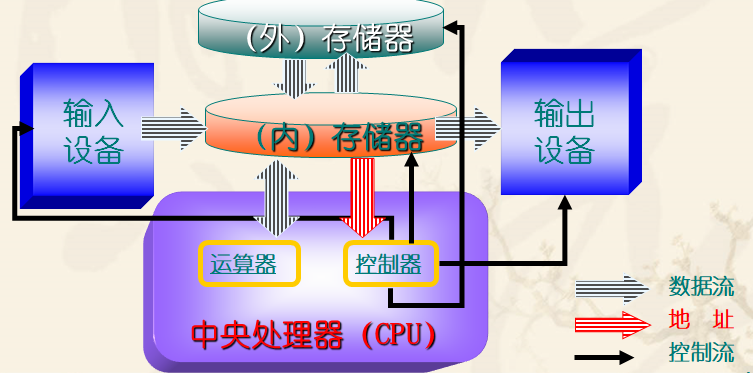
\includegraphics[scale=0.25]{hframe}
\end{frame}

\begin{frame}[shrink]
\frametitle{10进制,2进制,16进制的幂展开式}
\begin{align*}
(D)_{10}&=D_{n-1}\times 10^{n-1}+D_{n-2}\times 10^{n-2}+\cdots+D_{1}\times 10^{1}+D_{0}\times 10^{0}\\
&+D_{-1}\times 10^{-1}+D_{-2}\times 10^{-2}+\cdots+D_{-m+1}\times 10^{-m+1}+D_{-m}\times 10^{-m}\\
(B)_{2}&=B_{n-1}\times 2^{n-1}+B_{n-2}\times 2^{n-2}+\cdots+B_{1}\times 2^{1}+B_{0}\times 2^{0}\\
&+B_{-1}\times 2^{-1}+B_{-2}\times 2^{-2}+\cdots+B_{-m+1}\times 2^{-m+1}+B_{-m}\times 2^{-m}\\
(H)_{2}&=H_{n-1}\times 16^{n-1}+H_{n-2}\times 16^{n-2}+\cdots+H_{1}\times 16^{1}+H_{0}\times 16^{0}\\
&+H_{-1}\times 16^{-1}+H_{-2}\times 16^{-2}+\cdots+16_{-m+1}\times 16^{-m+1}+H_{-m}\times 16^{-m}
\end{align*}
\end{frame}

\begin{frame}{进制对照表}
\begin{tabular}{|c|c||c|c|}
	\hline 
	二进制 & 十六进制 & 二进制 & 十六进制 \\ 
	\hline 
	0000 &  0 & 1000  & 8 \\ 
	\hline 
	0001 &  1 & 1001  & 9 \\ 
	\hline 
	0010 &  2 & 1010  & A \\ 
	\hline 
	0011 &  3 & 1011  & B \\ 
	\hline 
	0100 &  4 & 1100  & C \\ 
	\hline 
	0101 &  5 & 1101  & D \\ 
	\hline 
	0110 &  6 & 1110  & E \\ 
	\hline 
	0111 &  7 & 1111  & F \\ 
	\hline 
\end{tabular} 
\end{frame}

\begin{frame}
\begin{example}
	\begin{align*}
	(123)_{10}&=1\times 10^2+2\times 10^1+3\times 10^0; \\
	&3=123\%10, 2=123/10\%10, 1=123/10/10\%10\\
	\newline
	(77)_{10}&=(0100\quad 1101)_{2}=0\times 2^7+1\times 2^6+0\times 2^5+0\times 2^4\\
	&+1\times 2^3+1\times 2^2+0\times 2^1+1\times 2^0\\
	\newline
	(77)_{10}&=(4D)_{16}=4\times 16^1+13\times 16^0
	\end{align*}
\end{example}
\end{frame}

\begin{frame}{数值在计算机中的表示(以8bit编码为例)}
\begin{itemize}
	\item 原码:正数的符号为0,负数的符号为1,其它位按一般的方法表示数的绝对值。
	\begin{align*}
	x=(+103)_{10}  &&[x]_{\text{原}}=(01100111)_{2}\\
	x=(-103)_{10}  &&[x]_{\text{原}}=(11100111)_{2}
	\end{align*}
	\item 反码: 正数的反码与原码相同;负数的反码是符号位不变,其他位按位取反 
	\item 补码: 正数的补码与其原码相同;负数的补码为其反码最末位加1. 即, \textcolor{blue}{补码 = 反码+1}
\end{itemize}
\begin{align*}
(77)_{10}&=(0100\quad 1101)_{2},\qquad (-77)_{10}=(1100\quad 1101)_{2}\\
(-77)_{\text{补}}=2^8-77&=1111\quad 1111 - 0100\quad 1101 +0000\quad 0001\\
	&=1011\quad 0010 + 0000\quad 0001=1011\quad 0011
\end{align*}
\end{frame}

\begin{frame}{机内以补码形式存储有符号数}
\begin{enumerate}
	\item 对于正数,原码=反码=补码
	\item 对于负数,补码=反码 + 1\\
	      反码 = 符号位不变, 其他位按位取反
	\item 补码是可逆的,即再对补码求补得到原码。
	\item 引入补码后,使减法统一为加法。	
\end{enumerate}
\end{frame}

\begin{frame}{数值表示示例}
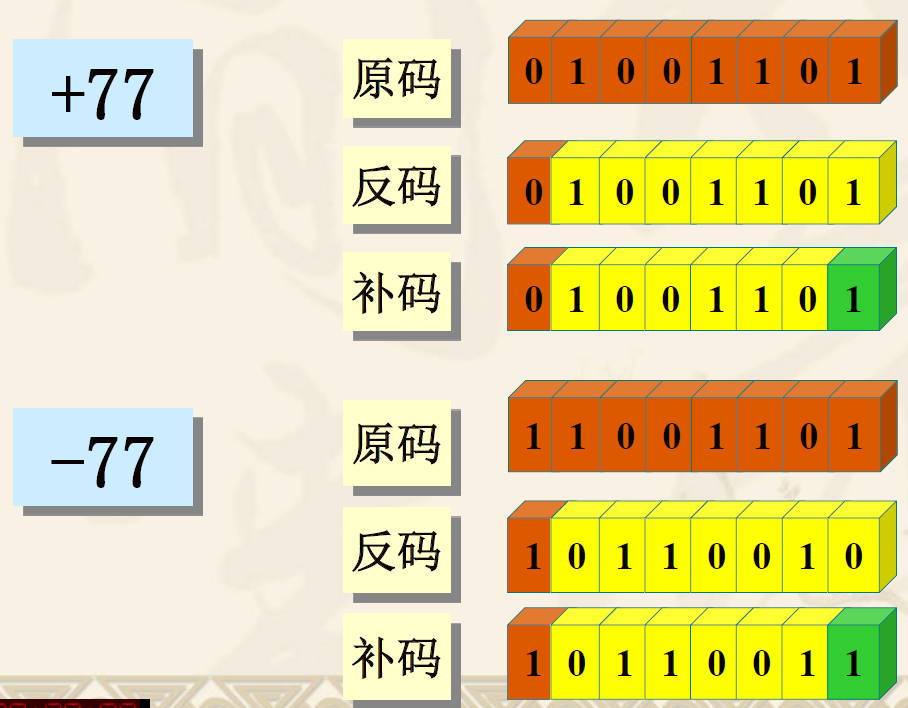
\includegraphics[scale=0.25]{2}
\end{frame}

\begin{frame}{ASCII编码表$B_6B_5B_4B_3B_2B_1B_0$}
\begin{columns}
	\column{0.7\textwidth}
	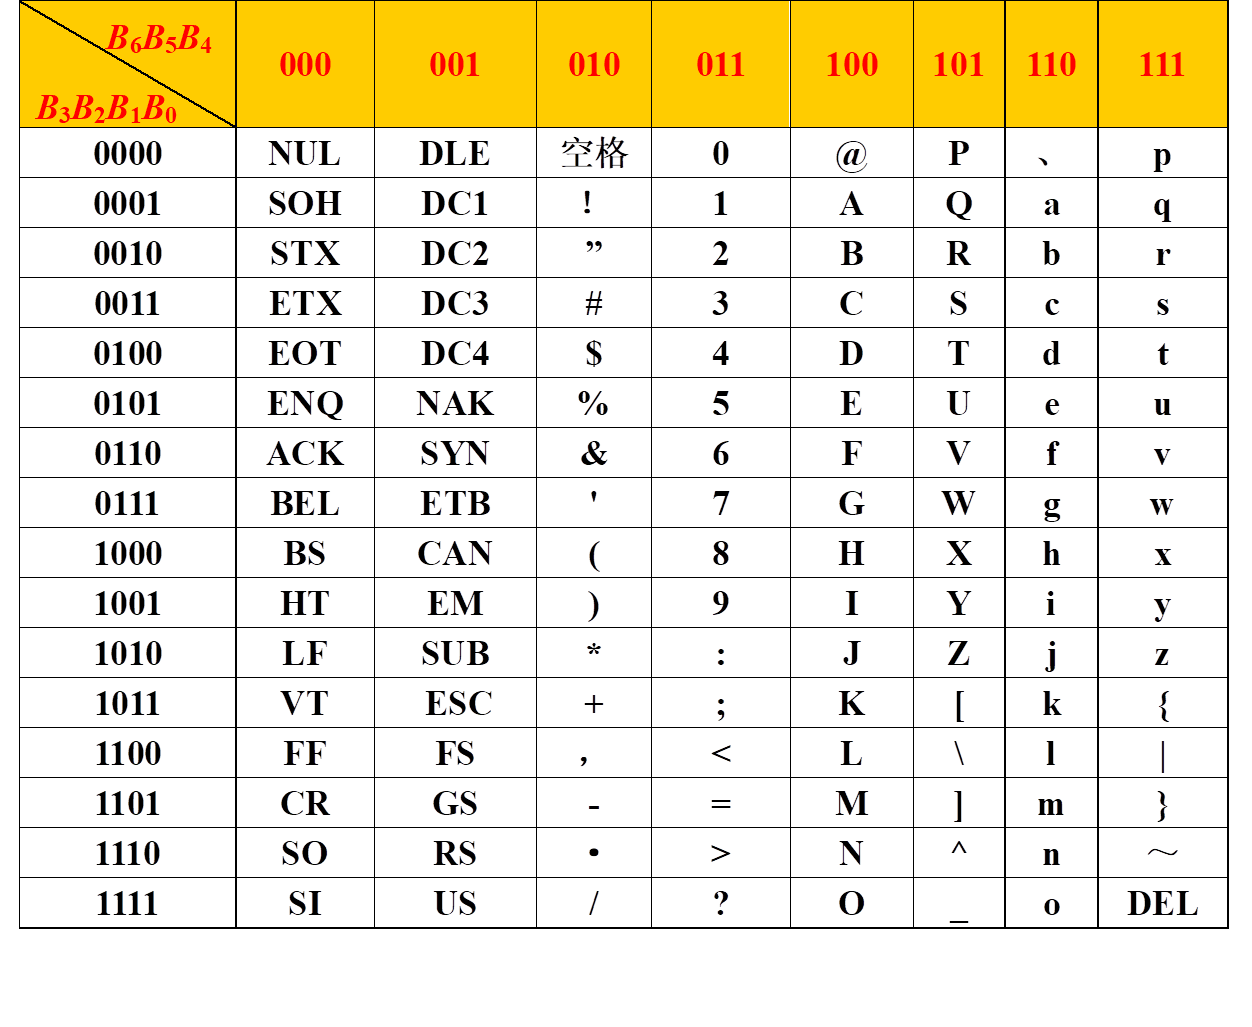
\includegraphics[scale=0.4]{ASCII}
	\column{0.3\textwidth}
	\begin{itemize}
		\item ASCII码连续排列 \\
		 `0'$\sim$`9', `A'$\sim$`Z', `a'$\sim$`z'
		\item 数字 = 编码值 - `0' \\
		 9=`9'-`0'
		\item 大小字符间隔: \\
		`a' - `A' = 32
	\end{itemize}	
\end{columns}
\end{frame}

\section{C语言程序设计}

\begin{frame}{计算机程序}

\includegraphics[scale=0.4]{program1}
\end{frame}

\begin{frame}{计算机语言}
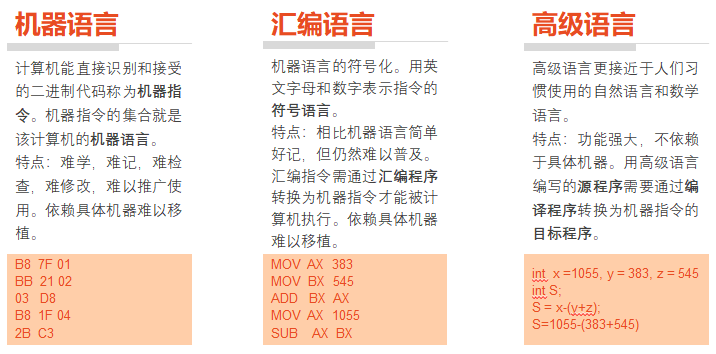
\includegraphics[scale=0.4]{program2}
\end{frame}

\begin{frame}{高级语言的发展}
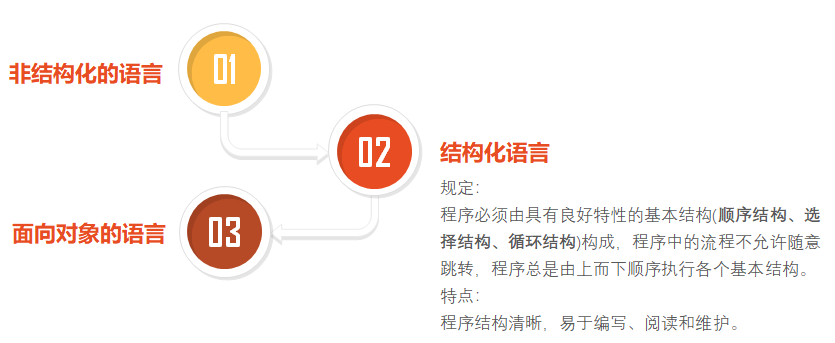
\includegraphics[scale=0.4]{program3}
\end{frame}

\begin{frame}{C语言的特点}
\begin{enumerate}
	\item 语言简洁、紧凑,使用方便、灵活
    \item 运算符丰富
    \item 数据类型丰富
    \item \textcolor{blue}{C语言是完全模块化和结构化的语言}\\
          具有结构化的控制语句(顺序、选择、循环结构)\\
          用函数作为程序的模块单位,便于实现程序的模块化
    \item \textcolor{blue}{兼具高级语言和低级语言的功能}\\
          允许直接访问物理地址\\
          能进行位(bit)操作\\  
          能实现汇编语言的大部分功能\\
          可以直接对硬件进行操作        
\end{enumerate}
\end{frame}

\begin{frame}{程序设计的任务}
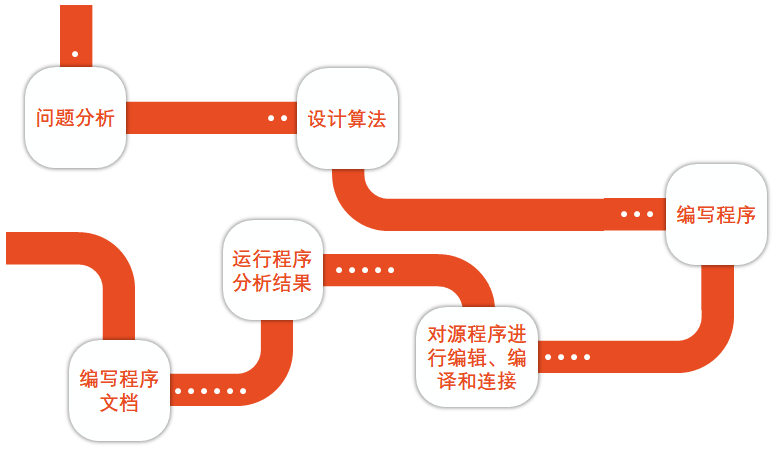
\includegraphics[scale=0.4]{program}
\end{frame}

\begin{frame}[fragile]{第一个C语言程序}
    \begin{lstlisting}
    #include<stdio.h>            // standard input/output编译预处理指令
    int main()                   // 主函数
    {                            // 函数开始标志
       printf("Hello World!");   // 输出一行信息
       return 0;                 // 函数执行完毕返回函数值0
    }                            // 函数结束标志
    \end{lstlisting}
\end{frame}

\begin{frame}[fragile]{求两个整数之和}
\begin{lstlisting}
#include<stdio.h>            // standard input/output编译预处理指令
int main()                   // 主函数
{                            // 函数开始标志
   int a,b,sum;           // 定义a,b,sum为整型变量
   a=123;                 // 对a,b赋值
   b=456;
   sum=a+b;              // 计算a+b, 并把结果存放在变量sum中
   printf("sum is %d\n",sum);   // 输出结果
   return 0;                 // 函数执行完毕返回函数值0
}                            // 函数结束标志
\end{lstlisting}
\end{frame}

\begin{frame}{运行C程序的步骤与方法}
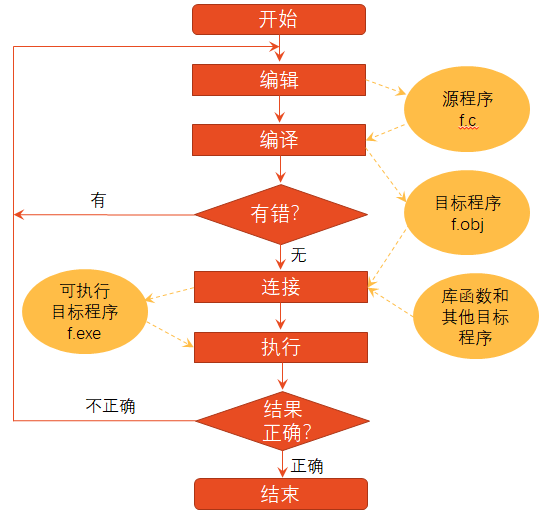
\includegraphics[scale=0.45]{program4}
\end{frame}

\begin{frame}{集成开发环境---编译系统}
\begin{itemize}
	\item Bloodshed Dev-C++ 
	\item Turbo C
	\item Visual C++6.0 
	\item Visual Studio(VS2015,VS Community 2019等)
\end{itemize}
\end{frame}

\begin{frame}{Bloodshed Dev-C++集成开发环境}
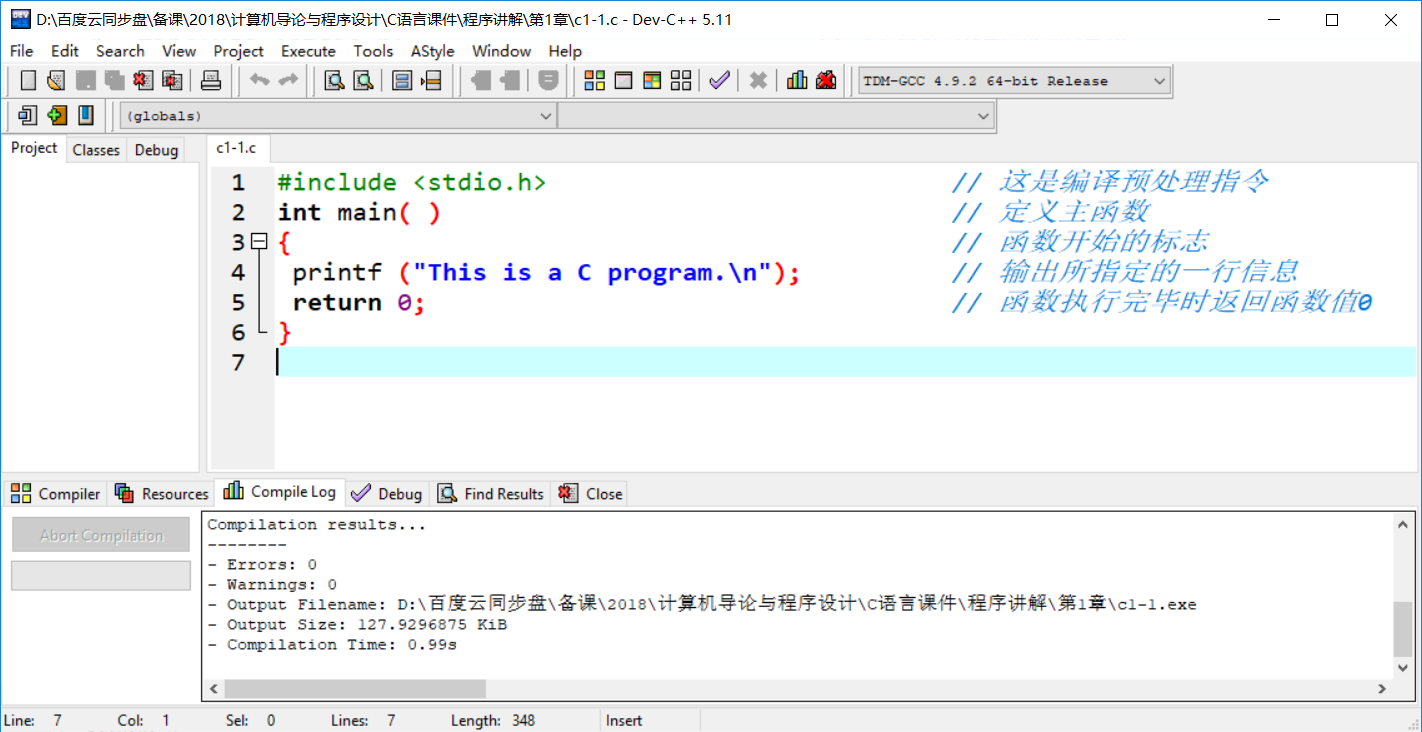
\includegraphics[scale=0.3]{DevCpp}   
\end{frame}

\begin{frame}{Bloodshed Dev-C++集成开发环境}
\begin{itemize}
	\item 选择“文件”菜单,选择“源文件”, 编辑程序。
	\item 保存时,保存为 .cpp或 .c文件。
	\item 选择“编译和运行”菜单,生成.exe文件,运行程序。  
\end{itemize} 
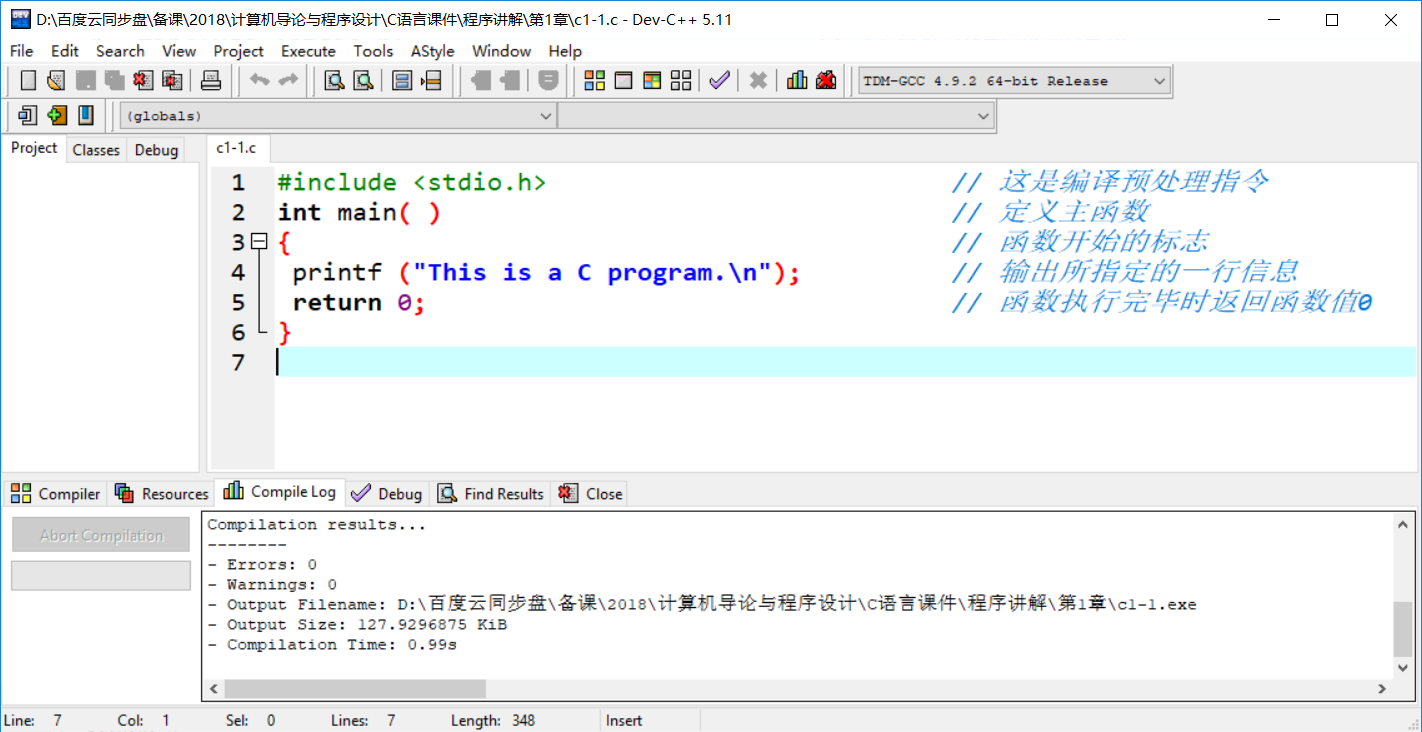
\includegraphics[scale=0.2]{DevCpp}   
\end{frame} % 课程介绍,导论简介, C语言程序设计
%%%%%%%%%%%%%%%%%%%%%%%%%%% lecture-2
%\begin{frame}
%  \frametitle{lecture-2 算法---程序的灵魂}
%  \tableofcontents[hideallsubsections]
%\end{frame}

\section{数据类型}

\begin{frame}{基本数据类型}
\begin{itemize}
	\item 整数\lstinline|int|
	\item 单精度浮点数\lstinline|float|
	\item 双精度浮点数\lstinline|double|
	\item 字符\lstinline|char|
\end{itemize}
\textcolor{red}{机内用二进制表示, 不同数据类型占用存储空间大小不同。}
\end{frame}

\begin{frame}[fragile]{变量在使用之前首先要定义它的数据类型}
\begin{lstlisting}
#include<stdio.h>            // standard input/output编译预处理指令
int main()                   // 主函数
{                            // 函数开始标志
	int a,b;  // 定义变量a, b为整型数值,同类型变量可以在一条语句中定义。
	float f;  // 定义变量f为单精度浮点数
	double d; // 定义变量d为双精度浮点数
	char c;   // 定义变量c为单个英文字母
	a=10;	  // 变量赋值
	b=20;
	f=10.2;
	d=20.3;
	c='A';	  // 字符用单引号括起来
	return 0;                // 函数执行完毕返回函数值0
}                            // 函数结束标志
\end{lstlisting}
\end{frame}

\begin{frame}[fragile]{标识符}
标识符就是一个对象的名字。用于标识变量、符号常量、函数、数组、类型等。\\
\textcolor{blue}{以字母或下划线开始; 区分大小写; 不能使用关键字; 最好有含义。}
\begin{lstlisting}
#include<stdio.h>           
int main()                   
{                            
	int r = 123; // 合法整型变量名
	int 3a; // 不合法的变量名
	int break; // 不合法的变量名, 因为break是关键字, 被系统使用。
	int Radius; // 变量名最好有含义
	int radius; // 与Radius是不同的变量,C语言是大小写敏感的语言
	return 0;           
}                            
\end{lstlisting}
\end{frame}

\begin{frame}{C语言关键字}
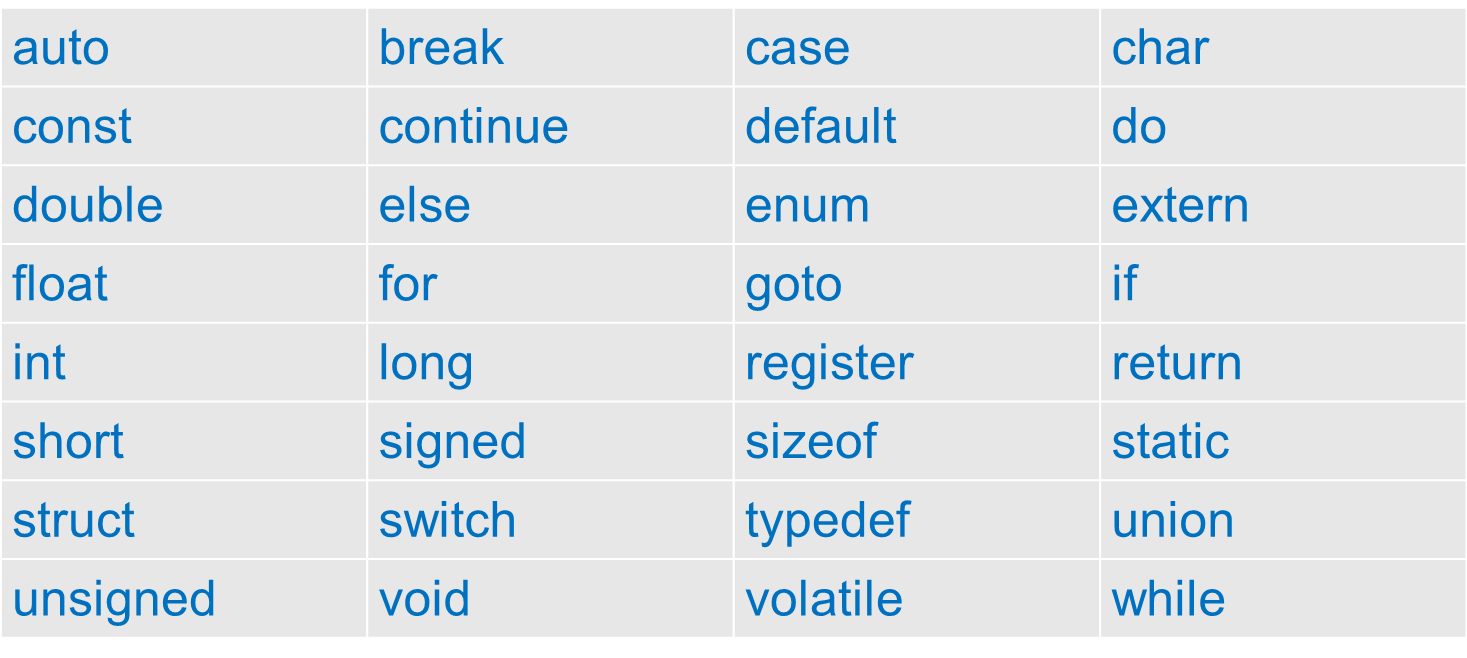
\includegraphics[scale=0.5]{key}
\end{frame}

\begin{frame}[shrink,fragile]{输出语句printf(``原样输出, \%格式符'', 对应变量值);}
\begin{lstlisting}
#include<stdio.h>            // standard input/output编译预处理指令
int main()                   // 主函数
{                            // 函数开始标志
	int a=10,b;    // 定义变量a, b为整型数值, 定义变量时,可以指定变量的初值
	float f=10.2;  // 定义变量f为单精度浮点数
	double d; // 定义变量d为双精度浮点数
	char c;   // 定义变量c为单个英文字母
	f=10.2;
	d=20.356;
	c='A';
	printf("a=%d,b=%d,c=%c,f=%f,d=%.2lf\n",a,b,c,f,d); // %.2f, %.2lf保留两位小数, \n为换行符
	return 0;                // 函数执行完毕返回函数值0
}                            // 函数结束标志
\end{lstlisting}
\textcolor{blue}{变量b没有被赋值, 将是一个随机值。}
\end{frame}

\begin{frame}{常用格式描述符与数据类型的对应关系}
\centering
\begin{tabular}{|c|c|c|}
	\hline 
	\textbf{格式符} & \textbf{对应的数据类型} &  \textbf{备注}\\ 
	\hline 
	\%d & int &  \\ 
	\hline  
	\%f & float &  \\
	\hline
	\%c & char & \\ 
	\hline   
	\%lf & double & \\ 
	\hline 
	\%.2f & float & 保留两位小数, 四舍五入。不适用于scanf()。 \\ 
	\hline 
	\%.2lf & double & 保留两位小数, 四舍五入。不适用于scanf()。 \\ 
	\hline   
	\%x(\%X) & int,char & 十六进制显示(大写) \\ 
	\hline 
	\%ld & long int &  \\ 
	\hline 
\end{tabular}
\newline
\newline
\textcolor{blue}{详见p73, 表3.6}
\end{frame}


\begin{frame}{十进制与二进制}
\vspace{-1cm}
\begin{align*}
&\textcolor{red}{\text{十进制: 以10为底的幂展开式:}}\\
&(123)_{10}=1\times 10^2+2\times 10^1+3\times 10^0; \\
&\textcolor{blue}{\text{自低到高各位数(除10取余至商为0): }3=123\%10,~2=123/10\%10=12\%10,}\\
&\textcolor{blue}{1=123/10/10\%10=1\%10}\\
&\textcolor{red}{\text{二进制: 以2为底的幂展开式:}}\\
&(77)_{10}=(0100\quad 1101)_{2}=0\times 2^7+1\times 2^6+0\times 2^5+0\times 2^4\\
&\qquad +1\times 2^3+1\times 2^2+0\times 2^1+1\times 2^0\\
&\textcolor{blue}{\text{自低到高各位数(除2取余至商为0): }1=77\%2,~0=77/2\%2=38\%2,}\\
&\textcolor{blue}{~1=77/2/2\%2=19\%2,~1=77/2/2/2\%2=9\%2,}\\
&~\textcolor{blue}{0=77/2/2/2/2/\%2=4\%2,~0=77/2/2/2/2/2/\%2=2\%2,\dots}\\
\end{align*}
\end{frame}

\begin{frame}[shrink]
\frametitle{10进制、2进制、16进制的幂展开式}
\vspace{-0.5cm}
\begin{align*}
(D)_{10}&=D_{n-1}\times 10^{n-1}+D_{n-2}\times 10^{n-2}+\cdots+D_{1}\times 10^{1}+D_{0}\times 10^{0}\\
&+D_{-1}\times 10^{-1}+D_{-2}\times 10^{-2}+\cdots+D_{-m+1}\times 10^{-m+1}+D_{-m}\times 10^{-m}\\
&\\
(B)_{2}&=B_{n-1}\times 2^{n-1}+B_{n-2}\times 2^{n-2}+\cdots+B_{1}\times 2^{1}+B_{0}\times 2^{0}\\
&+B_{-1}\times 2^{-1}+B_{-2}\times 2^{-2}+\cdots+B_{-m+1}\times 2^{-m+1}+B_{-m}\times 2^{-m}\\
&\\
(H)_{16}&=H_{n-1}\times 16^{n-1}+H_{n-2}\times 16^{n-2}+\cdots+H_{1}\times 16^{1}+H_{0}\times 16^{0}\\
&+H_{-1}\times 16^{-1}+H_{-2}\times 16^{-2}+\cdots+16_{-m+1}\times 16^{-m+1}+H_{-m}\times 16^{-m}
\end{align*}
\end{frame}

\begin{frame}{进制对照表$2^32^22^12^0=8+4+2+1$}
\centering
\begin{tabular}{|>{\columncolor{yellow}}c|c|c||>{\columncolor{yellow}}c|c|c|}
\hline 
十进制 & 二进制 & 十六进制 & 十进制 & 二进制 & 十六进制 \\ 
\hline 
0 & 0000 &  0 & 8 & 1000  & 8 \\ 
\hline 
1 & 0001 &  1 & 9 & 1001  & 9 \\ 
\hline 
2 & 0010 &  2 & 10 & 1010  & A \\ 
\hline 
3 & 0011 &  3 & 11 & 1011  & B \\ 
\hline 
4 & 0100 &  4 & 12 & 1100  & C \\ 
\hline 
5 & 0101 &  5 & 13 & 1101  & D \\ 
\hline 
6 & 0110 &  6 & 14 & 1110  & E \\ 
\hline 
7 & 0111 &  7 & 15 & 1111  & F \\ 
\hline 
\end{tabular} 
\end{frame}

\begin{frame}{十进制、二进制与十六进制数值分解举例}
\vspace{-0.5cm}
\begin{align*}
(123)_{10}&=1\times 10^2+2\times 10^1+3\times 10^0; \\
&\textcolor{blue}{\text{自低到高各位数: }3=123\%10,~2=123/10\%10,~1=123/10/10\%10}\\
&\\
(77)_{10}&=(0100\quad 1101)_{2}=0\times 2^7+1\times 2^6+0\times 2^5+0\times 2^4\\
&+1\times 2^3+1\times 2^2+0\times 2^1+1\times 2^0\\
&\\
(77)_{10}&=(4D)_{16}=4\times 16^1+13\times 16^0
\end{align*}
\end{frame}

%\begin{frame}[shrink]{数值在计算机中的表示(以8bit编码为例)}
%\begin{itemize}
%	\item 原码:正数的符号为0,负数的符号为1,其它位按一般的方法表示数的绝对值。
%	\vspace{-0.5cm}
%	\begin{align*}
%	x=(+103)_{10}  &&[x]_{\text{原}}=(\textcolor{red}{0}1100111)_{2}\\
%	x=(-103)_{10}  &&[x]_{\text{原}}=(\textcolor{red}{1}1100111)_{2}
%	\end{align*}
%	\item 反码: 正数的反码与原码相同;负数的反码是符号位不变,其他位按位取反 
%	\item 补码: 正数的补码与其原码相同;负数的补码为其反码最末位加1. 即,
%	
%	\textcolor{blue}{负数补码 = 反码$+1=2^n-$该数的绝对值, $n$是编码二进制位数.}
%\end{itemize}
%\vspace{-0.5cm}
%\begin{align*}
%(77)_{10}&=(\textcolor{red}{0}100\quad 1101)_{2},\qquad (-77)_{10}=(\textcolor{red}{1}100\quad 1101)_{2}\\
%(-77)_{\text{补}}=2^8-77&=\textcolor{red}{1}111\quad 1111 +\textcolor{red}{0}000\quad 0001 - \textcolor{red}{0}100\quad 1101\\
%&=\underbrace{\textcolor{red}{1}111\quad 1111 - \textcolor{red}{0}100\quad 1101}_{(-77)_{\text{反}}} + ~\textcolor{red}{0}000\quad 0001\\
%&=\underbrace{\textcolor{red}{1}011\quad 0010 }_{(-77)_{\text{反}}}+ \textcolor{red}{0}000\quad 0001=1011\quad 0011
%\end{align*}
%\end{frame}

\begin{frame}[shrink]{数值在计算机中的表示(以8bit编码为例)}
\begin{tikzpicture}
\node[text width=1\textwidth] (t) {
\begin{itemize}
	\item 原码:正数的符号为0,负数的符号为1,其它位按一般的方法表示数的绝对值。
	\vspace{-0.5cm}
	\begin{align*}
	x=(+103)_{10}  &&[x]_{\text{原}}=(\textcolor{red}{0}1100111)_{2}\\
	x=(-103)_{10}  &&[x]_{\text{原}}=(\textcolor{red}{1}1100111)_{2}
	\end{align*}
	\item 反码: 正数的反码与原码相同;负数的反码是符号位不变,其他位按位取反 
	\item 补码: 正数的补码与其原码相同;负数的补码为其反码最末位加1. 即,
	
	\textcolor{blue}{负数补码 = 反码$+1=2^n-$该数的绝对值, $n$是编码二进制位数.}
\end{itemize}
\vspace{-0.5cm}
\begin{align*}
(77)_{10}&=(\textcolor{red}{0}100\quad 1101)_{2},\qquad (-77)_{10}=(\textcolor{red}{1}100\quad 1101)_{2}\\
(-77)_{\text{补}}=2^8-77&=\textcolor{red}{1}111\quad 1111 +\textcolor{red}{0}000\quad 0001 - \textcolor{red}{0}100\quad 1101\\
&=\underbrace{\textcolor{red}{1}111\quad 1111 - \textcolor{red}{0}100\quad 1101}_{(-77)_{\text{反}}} + ~\textcolor{red}{0}000\quad 0001\\
&=\underbrace{\textcolor{red}{1}011\quad 0010 }_{(-77)_{\text{反}}}+ \textcolor{red}{0}000\quad 0001=1011\quad 0011
\end{align*}
};
\node[anchor=south west,text width=.4\textwidth] at($(t.south west)+(0.2cm,0.2cm)$) {
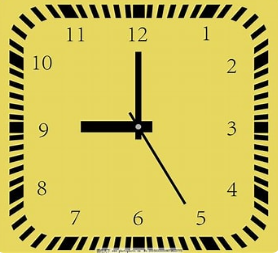
\includegraphics[scale=0.2]{clock}
};
\end{tikzpicture}
\end{frame}

\begin{frame}{数值表示示例}
\centering
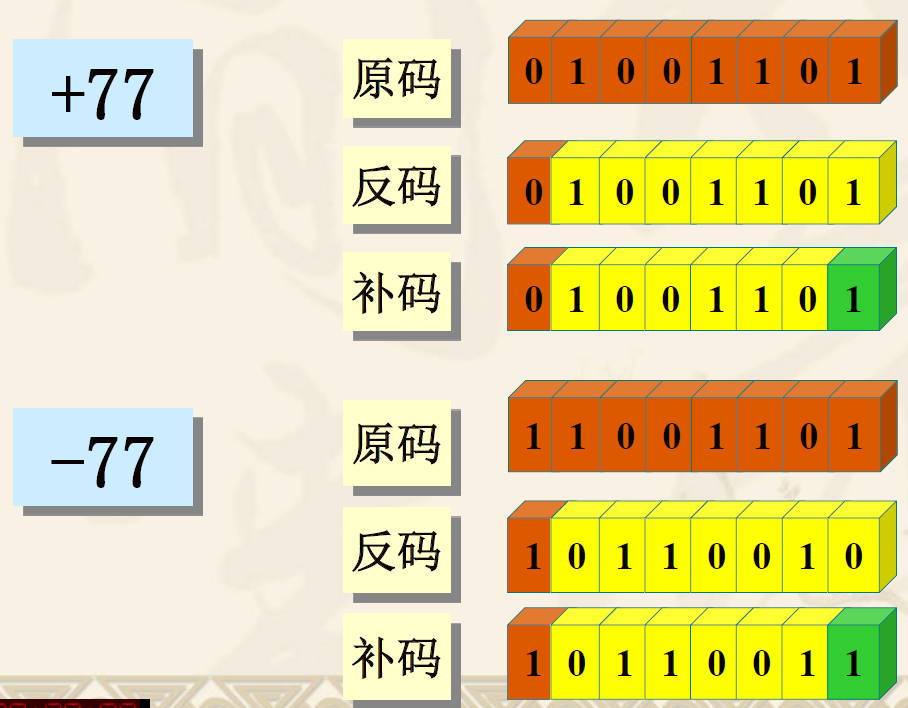
\includegraphics[scale=0.25]{2}
\end{frame}

\begin{frame}{机内以补码形式存储有符号数}
\begin{enumerate}
\setlength{\itemsep}{.5cm}
\item 对于正数,原码=反码=补码
\item 对于负数,补码=反码 + 1\\
反码 = 符号位不变, 其他位按位取反
\item 补码是可逆的,即再对补码求补得到原码。
\item 引入补码后,使减法统一为加法。
$(+77)_{\text{补}}+(-77)_{\text{补}}=0100~1101+1011~0011=0000~0000$	

\textcolor{blue}{注意: 由于采用8bit编码, 从右到左的第9位的1被舍弃。}
\end{enumerate}
\end{frame}

\note
{
0原码是00000000 -0原码是10000000

0反码是00000000 -0反码是11111111

0补码是00000000 补码没有正0与负0之分。+0和-0的补码是一样的。即 0的补码只有一种表示。

+0的补码:00000000

-0的补码:第一步:11111111 第二步+1= 1 00000000 第三部:进位1被丢弃 您明白了吗?

在规定中,8位二进制码能表示的反码范围是-127~127。

此时(字长为8位), -128没有原码和反码(只有补码)。

那么,为什么规定字长8位时-128没有原码和反码呢?下面解释。

首先看-0,[-0]原码=1000 000,其中1是符号位,求反操作,算出[-0]反码=1111 1111,

再看-128,假如它有原码且[-128]原码=1000~000,假如让-128也有反码,求反操作,则[-128]反码=1111~1111,

你会发现,-128的反码和-0的反码相同,所以为了避免面混淆,有了-0的原码,便不能有-128的原码补码,这是8位比特位位数限制决定的。
}

\begin{frame}{补码运算实例(以8bit编码为例)}
\textcolor{blue}{补码可逆:}
\begin{align*}
&[-25]_{\text{原}}=(1001~1001)_2\quad [-25]_{\text{反}}=(1110~0110)_2\\
&[-25]_{\text{补}}=[-25]_{\text{反}}+1=(1110~0110+1)_2=(1110~0111)_2\\
&[-25]_{\text{原}}=\left([-25]_{\text{补}}\right)_{\text{补}}=(1001~1000+1)_2=(1001~1001)_2
\end{align*}

\textcolor{blue}{减法统一为加法: $[a-b]_{\text{补}}=a_{\text{补}}+[-b]_{\text{补}}$}
\begin{align*}
&[102-25]_{\text{补}}=[77]_{\text{补}}=(0100~1101)_2=77\\
&[102]_{\text{补}}+[-25]_{\text{补}}=(0110~0110)_2+(1110~0111)_2=(0100~1101)_2=77\\
&\text{所以, }[102-25]_{\text{补}}=[102]_{\text{补}}+[-25]_{\text{补}}\\
&\text{同样有, }[25-102]_{\text{补}}=[25]_{\text{补}}+[-102]_{\text{补}}\\
\end{align*}
\end{frame}

\begin{frame}{计算机数据存储单位}
位(bit)是最小的存储单位,每一位存储1位二进制码, 一个字节(Byte)由8位组成。
\begin{itemize}
	\item 1B = 8b
	\item 1KB = 1024B
	\item 1MB = 1024KB
	\item 1GB = 1024MB
	\item 1TB = 1024GB
\end{itemize}
\end{frame}

\note{ 1B = $2^3$b (8位), 1KB = $2\times 2^8$ = $2^10$ B}

\begin{frame}[shrink,fragile]{整型数据输出printf(``\%d,\%x'', -25, -25);}
\vspace{-0.7cm}
\begin{center}
\begin{tikzpicture}
\node[text width=1.0\textwidth] (p) {
	\begin{lstlisting}[framextopmargin=1mm]
	#include<stdio.h>            // standard input/output编译预处理指令
	int main()                   
	{                            
		int a=-25,b=102;    // 定义变量a, b为整型数值, 定义变量时,可以指定变量的初值
		printf("a=%d,b=%d,a=%x,b=%x\n",a,b,a,b); 
		printf("%d,%d,%x,%x\n",-25,102,-25,102); 
		printf("%d,%d,%x,%x,%X\n", 77,-77,77,-77,-77);
		return 0;                
	}                            
	\end{lstlisting}
};

\node[anchor=north west,text width=.5\textwidth,draw,rounded corners,fill=black,white] (r) at(p.south west) {
	// 编译运行, 解释输出结果。
	\begin{verbatim*}
	a=-25,b=102,a=ffffffe7,b=66
	-25,102,fffffe7,66
	77,-77,4d,ffffffb3,FFFFFFB3
	\end{verbatim*}
};

\node[anchor=north west,text width=.5\textwidth,draw,rounded corners,fill=green] at(r.north east) {
	$[-25]_{\text{补}}=(1110~0111)_2=\text{E7H (0XE7)}$
	
	$[-77]_{\text{补}}= (1011~0011)_2=\text{B3H (0XB3)}$
	
	$66\text{H}=6\times 16^1+6\times 16^0=102$
	
	$4\text{DH}=4\times 16^1+13\times 16^0=77$
};
\end{tikzpicture}
\end{center}
\end{frame}

%\begin{frame}[fragile]{bbb}
%%\begin{center}
%	\begin{tikzpicture}[outer xsep=5pt]
%	\node[draw,text width=0.5\textwidth]{ \begin{lstlisting}
%		aa
%		\end{lstlisting}
%	};
%	\end{tikzpicture}
%	
%%\end{center}
%\end{frame}


\note{
	\begin{lstlisting}
	printf("%d,%x,%X\n",-25,-25,-25); // -25,ffffffe7,FFFFFFE7
	printf("%d,%x,%X\n",-77,-77,-77); // -77,ffffffb3,FFFFFFB3}
	\end{lstlisting}
}

\begin{frame}{ASCII编码表$B_6B_5B_4B_3B_2B_1B_0$}
\begin{columns}
	\column{0.65\textwidth}
	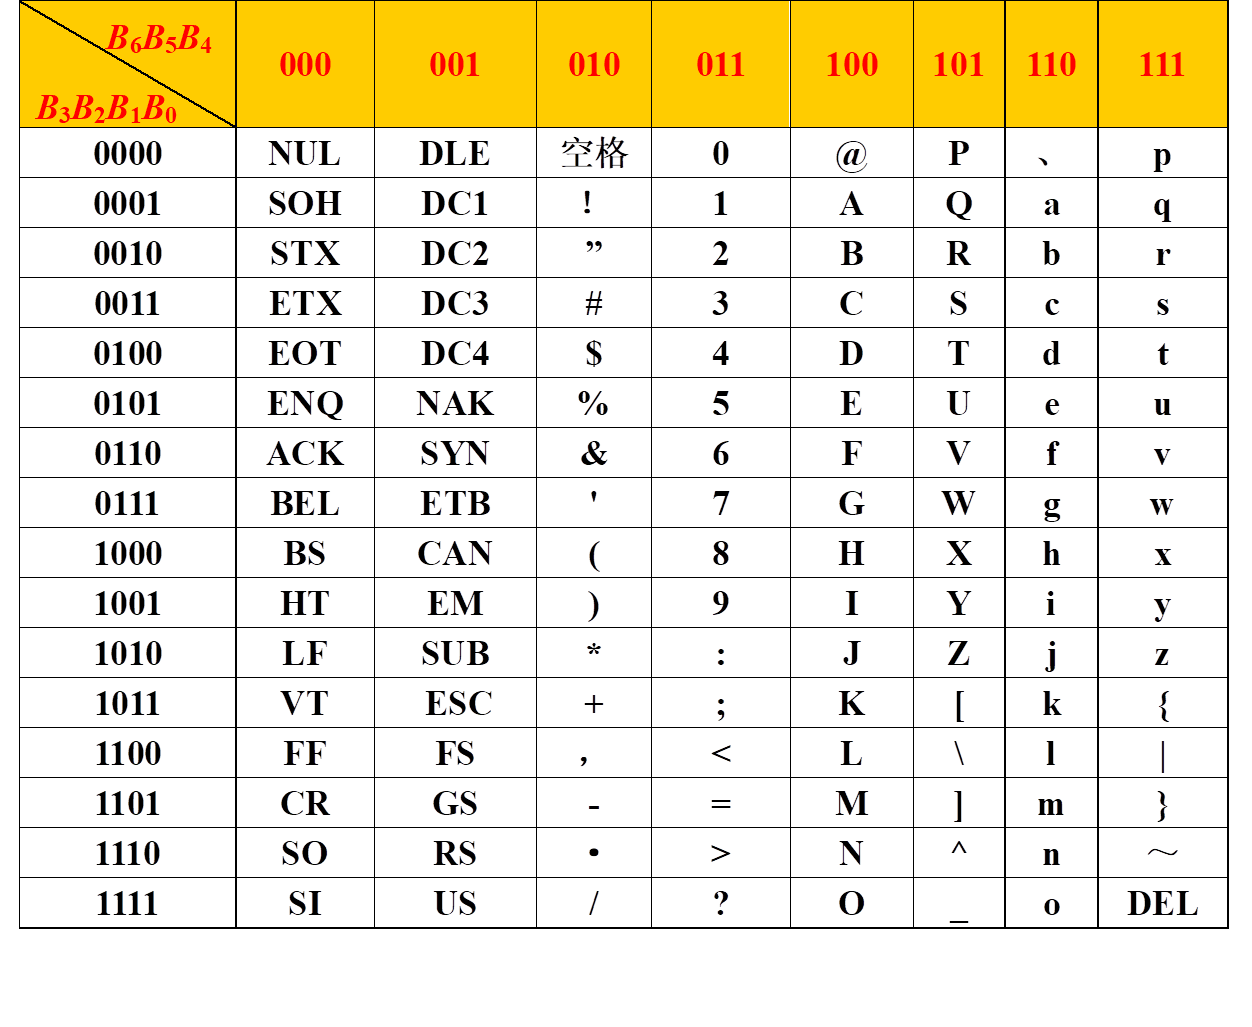
\includegraphics[scale=0.4]{ASCII}
	\column{0.35\textwidth}
	\begin{itemize}
		\item ASCII码连续排列 \\
		`0'$\sim$`9', `A'$\sim$`Z', `a'$\sim$`z'
		\item 数字 = 编码值 - `0' \\
		9=`9'-`0'
		\item 大小字符间隔: \\
		`a' - `A' = 32
		
		\scriptsize{
			`a'=0110~0001=61H=0X61=97
			
			'A'=0100~0001=41H=0X41=65}
	\end{itemize}	
\end{columns}
\end{frame}

\begin{frame}[shrink,fragile]{字符类型}
\begin{lstlisting}
#include<stdio.h>           
int main()                   
{                            
	char c1 = 'A', c2 = 'a', c3 = '\n'; // 字符型变量, 
	// '\n': 表示特殊字符 --- 换行符
	printf("%c,%c,%d\n",c1,c2,c3); // A,a,10
	// 整型变量的整数值就是ASCII编码值
	printf("%c,0X%x,%d\n",c1,c1,c1); // A,0X41,65
	c1 = c1 + 1; // 在表达式中, char类型当作int处理
	printf("%c,0X%x,%d\n",c1,c1,c1); // B,0X42,66
	c1 = c1 + 32;  // 转换为小写字母
	printf("%c,0X%x,%d\n",c1,c1,c1); // b,0X62,98
	printf("%d\n",'9'-'0'); // 数字 = 编码值- '0'
	printf("%c,%d,%c,%d\n",'A','A','a','a'); // 输出字符和相应的ASIII编码
	return 0;           
}                            
\end{lstlisting}
\end{frame}


\begin{frame}[shrink,fragile]{常量}
\vspace{-0.2cm}
\begin{lstlisting}
#include<stdio.h> 
#define PI 3.14  // 符号常量, 注意没有分号           
int main()                   
{                                  
	int a = 123; // 整型常量
	float f = 12.2, f1=123E-1; // 实型常量, $123\times 10^{-1}$
	char c1 = 'A', c2='\n'; // 字符常量, 特殊字符 --- 换行符
	char s[50] = "boy"; // 字符串常量
	printf("半径为%d的圆周长是%f\n",a,2*PI*a);       
	printf("回车换行\n");
	printf("单引号\',双引号\"转义字符前缀\,\n");  
	return 0;           
}                            
\end{lstlisting}
\textcolor{blue}{转义字符(特殊字符), 见p40, 表3.1}
\end{frame}

\begin{frame}[fragile]{常量与常变量}
\begin{lstlisting}
#include<stdio.h> 
#define PI 3.14  // 符号常量, 注意没有分号           
int main()                   
{                            
	int r = 123; // 整型变量
	const int a = 425; // 常变量
	r = 100; // 合法, 因为r是变量,可以随时更改它的值
	a = 100; // 不合法,因为a是常变量,不能更改
	printf("半径为%d的圆周长是%f\n",r,2*PI*r); 
	return 0;           
}                            
\end{lstlisting}
\end{frame}

\begin{frame}[fragile,shrink]{长整型、无符号整型, 浮点型数据类型}
\begin{lstlisting}
#include<stdio.h>           
int main()                   
{                            
	int a = 123; // 整型变量
	long int b = 1E+8; // 长整型变量
	unsigned int u = 0XFF; // 无符号整型, 最高位不作为符号位处理
	float f = 10.2; // 单精度浮点数
	double d = 1E-8; // 双精度浮点数
	printf("%x,%d\n",u,u); // ff, 255
	printf("%d,%ld,%x,%f,%lf\n",a,b,u,f,d);
	// sizeof函数返回类型分配的字节数,整型数据存储空间和值的范围见p45, 表3.2
	printf("%d,%d,%d,%d\n",sizeof(int),sizeof(float),sizeof(double),sizeof(long int),sizeof(long long int));
	return 0;           
}                            
\end{lstlisting}
\end{frame}



 % 开发工具,算法,初识C语言程序(作业)
%%%%%%%%%%%%%%%%%%%%%%%%%%% lecture-3
%\begin{frame}
%  \frametitle{lecture-3 主要内容}
%  \framesubtitle{最简单的C语言程序设计---顺序程序设计}
%  \tableofcontents[hideallsubsections]
%\end{frame}

\section{数据的输入输出}

\begin{frame}{常用格式描述符与数据类型的对应关系}
\begin{tabular}{|c|c|c|}
	\hline 
	\textbf{格式符} & \textbf{对应的数据类型} &  \textbf{备注}\\ 
	\hline 
	\%d & int &  \\ 
	\hline  
	\%f & float &  \\
	\hline
	\%c & char & \\ 
	\hline   
	\%lf & double & \\ 
	\hline 
	\%.2f & float & 保留两位小数, 四舍五入。不适用于scanf()。 \\ 
	\hline 
	\%.2lf & double & 保留两位小数, 四舍五入。不适用于scanf()。 \\ 
	\hline
	\hline   
	\%x & int & 十六进制显示 \\ 
	\hline 
	\%ld & long int &  \\ 
	\hline 
\end{tabular}
\newline
\newline
\textcolor{blue}{详见p73, 表3.6}
\end{frame}

\begin{frame}[shrink,fragile]{输出语句printf(``原样输出, \%格式符'', 对应变量值);}
\begin{lstlisting}
#include<stdio.h>            // standard input/output编译预处理指令
int main()                   // 主函数
{                            // 函数开始标志
   int a=10,b;    // 定义变量a, b为整型数值, 定义变量时,可以指定变量的初值
   float f=10.2;  // 定义变量f为单精度浮点数
   double d; // 定义变量d为双精度浮点数
   char c;   // 定义变量c为单个英文字母
   f=10.2;
   d=20.356;
   c='A';
   printf("a=%d,b=%d,c=%c,f=%f,d=%.2lf\n",a,b,c,f,d); // %.2f, %.2lf保留两位小数
   return 0;                 // 函数执行完毕返回函数值0
}                            // 函数结束标志
\end{lstlisting}
\textcolor{blue}{变量b没有被赋值, 将是一个随机值。}
\end{frame}

\begin{frame}[fragile]{输入语句scanf(``\%变量格式符'', \&变量名);}
\begin{lstlisting}
#include<stdio.h>            // standard input/output编译预处理指令
int main()                   // 主函数
{                            // 函数开始标志
   int a=10,b;    // 定义变量a, b为整型数值, 定义变量时,可以指定变量的初值
   float f=10.2;  // 定义变量f为单精度浮点数
   double d; // 定义变量d为双精度浮点数
   char c='A';   // 定义变量c为单个英文字母, 字符输入以后讲
   printf("请输入整数和浮点数, 空格隔开:\n"); // 提示语句[可选]
   scanf("%d%f",&a,&f);  // 尽量简单, 不要有其它字符和'\n'
   printf("请输入两个浮点数, 空格隔开:\n"); // 提示语句[可选]
   scanf("%f%lf",&f,&d);
   printf("a=%d,b=%d,c=%c,f=%f,d=%lf\n",a,b,c,f,d); // \n为换行符
   return 0;                 // 函数执行完毕返回函数值0
}                            // 函数结束标志
\end{lstlisting}
\end{frame}

\begin{frame}[fragile]{字符输出函数putchar}
\begin{lstlisting}
#include<stdio.h>
int main()
{
   char a = 'B',b = 'O',c = 'Y'; //定义3个字符变量并初始化
   putchar(a); //向显示器输出字符B
   putchar(b); //向显示器输出字符O
   putchar(c); //向显示器输出字符Y
   putchar ('\n'); //向显示器输出一个换行符
   return 0;
}
\end{lstlisting}
\end{frame}

\begin{frame}[fragile]{字符输入函数getchar, 遇到回车, 开始从缓冲区中接收字符。}
\vspace{-0.4cm}
\begin{lstlisting}
#include<stdio.h>
int main()
{
   char a,b,c;  //定义字符变量a,b,c
   a = getchar();  //从键盘输入一个字符,送给字符变量a
   b = getchar();  //从键盘输入一个字符,送给字符变量b
   c = getchar();  //从键盘输入一个字符,送给字符变量c
   putchar(a);  //将变量a的值输出
   putchar(b);  //将变量b的值输出 
   putchar(c);  //将变量c的值输出
   printf("\na=%d,b=%d,c=%d,a=%c,b=%c,c=%c\n",a,b,c,a,b,c);
   return 0;
}
\end{lstlisting}
\end{frame}

\begin{frame}[fragile]{\small 字符输入函数getchar, 遇到回车, 开始从缓冲区中接收字符。}
\begin{lstlisting}
char a,b,c;  //定义字符变量a,b,c
a = getchar();  //从键盘输入一个字符,送给字符变量a
b = getchar();  //从键盘输入一个字符,送给字符变量b
c = getchar();  //从键盘输入一个字符,送给字符变量c
putchar(a);  //将变量a的值输出
putchar(b);  //将变量b的值输出 
putchar(c);  //将变量c的值输出
printf("\na=%d,b=%d,c=%d,a=%c,b=%c,c=%c\n",a,b,c,a,b,c);
\end{lstlisting}
从键盘输入abc回车, 观察结果, 应该是正确的结果。
遇到回车, 开始从缓冲区中接收字符。
\end{frame}

\begin{frame}[fragile]{\small 字符输入函数getchar, 遇到回车, 开始从缓冲区中接收字符。}
\begin{lstlisting}
a = getchar();  //从键盘输入一个字符,送给字符变量a='a'
b = getchar();  //从键盘输入一个字符,送给字符变量b='\n'
c = getchar();  //从键盘输入一个字符,送给字符变量c='b'
putchar(a);  //将变量a的值输出a
putchar(b);  //将变量b的值输出\n 
putchar(c);  //将变量c的值输出b
printf("\na=%d,b=%d,c=%d,a=%c,b=%c,c=%c\n",a,b,c,a,b,c);
\end{lstlisting}
再运行一次程序, 输入a回车, 输入b回车, 输入c回车, 观察结果。\\
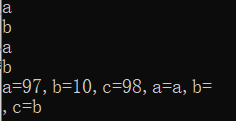
\includegraphics[scale=0.5]{abc}
\end{frame}

\begin{frame}{开发平台上演示讲解}
在开发平台,以具体的示例,详细讲解以下内容:
\begin{itemize}
	\item int, float, double, char 数据类型, sizeof(~)函数
	\item \%d, \%f, \%c, \%lf, \%x格式符的使用(见ppt中的表格)
	\item if(~)\{\quad\}, while(~)\{\quad\}简单语句
	\item char c; scanf(``\%c", \&c); 接收输入的字符
	\item char c; c=getchar()接收输入的字符, putchar()输出一个字符
	\item 编程理解数字ASCII码与整数的对应关系以及大小写字符之间的关系。
	\item 避免数字,字符在一条语句中输入的情况,如:\\ scanf(``\%d\%c\%d",...);
	\item 重点理解字符缓冲区的概念,以及消费无用字符的技巧。
\end{itemize}
\end{frame}

\note
{
根据学生的反馈,数据的输入语句没有完全听明白。 \\
下一讲, 进一步详细讲解。\\
欢迎同学们在群里踊跃发言,任何不理解的知识点请指出来,我将在以后的讲课中,有针对性的讲清楚大家有疑惑的问题。一些与编程无关的俏皮话之类的东西就不要发了,争取把我们这个群建立成纯净的,对大家学习课程有帮助的程序设计讨论群。力争100名学生一个都不掉队,考个好成绩。加油!!
}



 % 初识C语言程序(讲解作业), 数据的输入输出
%%%%%%%%%%%%%%%%%%%%%%%%%%% lecture-1
\begin{frame}[shrink]
  \frametitle{lecture-4 主要内容}
  \framesubtitle{选择结构程序设计}
  \tableofcontents[hideallsubsections]
\end{frame}

\section{选择结构和条件判断}

\begin{frame}{选择结构和条件判断}
\begin{columns}
	\column{0.6\textwidth}
	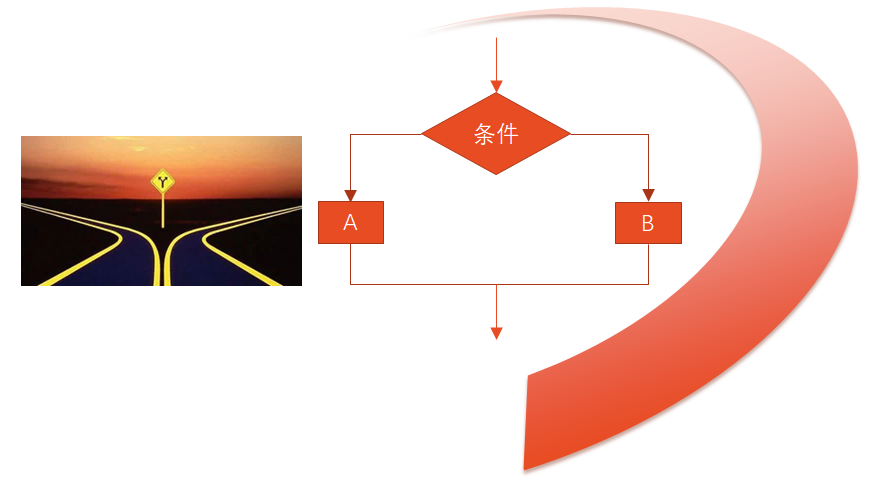
\includegraphics[scale=0.25]{if-case}
	\column{0.4\textwidth}
	\begin{block}{C语言有两种选择语句}
		\begin{itemize}
			\item if语句, 用来实现\textbf{两个分支}的选择结构
			\item switch语句, 用来实现\textbf{多分支}的选择结构
		\end{itemize}
	\end{block}
\end{columns}
\end{frame}

\begin{frame}[fragile]{if(条件表达式)\{ 表达式为真(非0)时执行语句; \}}
\begin{lstlisting}
#include<stdio.h>            // standard input/output编译预处理指令
int main()                   // 主函数
{                            // 函数开始标志
   int a=10;    // 定义变量a为整型数值, 定义变量时,可以指定变量的初值
   if(a>=10)
   {
      printf("a>=10\n"); // \n为换行符
   }
   else
   {
      printf("a<10\n"); // \n为换行符
   }
   return 0;                 // 函数执行完毕返回函数值0
}                            // 函数结束标志
\end{lstlisting}
\end{frame}

\begin{frame}[shrink,fragile]
\small [例4.1 p84] 求$ax^2+bx+c=0$方程的根。$a,b,c$由键盘输入。
\begin{lstlisting}
#include<stdio.h>
#include<math.h>   // 数学库函数        
int main()                   
{  
   double a,b,c,x1,x2,delta;
   scanf("%lf%lf%lf",&a,&b,&c);
   if(b*b-4*a*c < 0) 
   { printf("This equation hasn\'t real roots!\n"); }
   else
   {
      delta = sqrt(b*b-4*a*c);
      x1 = -b + delta/(2*a);  x2 = -b - delta/(2*a);
      printf("x1=%.2lf,x2=%.2lf\n",x1,x2);
   }
   return 0;           
}                            
\end{lstlisting}
\end{frame}

\begin{frame}[shrink,fragile]
\small [例4.2 p85] 输入两个实数, 按由小到大的顺序输出这两个数。
\begin{columns}
\column{0.45\textwidth}
\begin{lstlisting}
#include<stdio.h>        
int main()                   
{  
   float a,b,t;
   scanf("%f%f",&a,&b); 
   //不好: scanf("%f,%f",&a,&b);
   if(a>b)
   {  //将a和b的值互换
      t=a;
      a=b;
      b=t;
   }
   printf("%.2f,%.2f\n",a,b);
   return 0;           
}
\end{lstlisting} 
\column{0.55\textwidth}
\small
\begin{block}{两个变量值的互换}
a=b;  //把变量b的值赋给变量a,a的值等于b的值\\
b=a;  //再把变量a的值赋给变量b,变量b值没有改变
\end{block}
\textbf{因此, 为了实现互换, 必须借助于第三个变量。}
\end{columns}                           
\end{frame}

\begin{frame}[shrink,fragile]
\small [例4.3 p86] 输入3个数a, b, c, 要求按由小到大的顺序输出。
\begin{lstlisting}
#include<stdio.h>        
int main()                   
{  
    float a,b,c,t;
    scanf("%f%f%f",&a,&b,&c); //不好: scanf("%f,%f,%f",&a,&b,&c);
    if(a>b)
    {
       t=a; a=b; b=t; //借助变量t,实现变量a和变量b互换值
    } //互换后,a小于或等于b     
    if(a>c)
    {
       t=a; a=c; c=t; //借助变量t,实现变量a和变量c互换值
    } //互换后,a小于或等于c       
    if(b>c) //还要
    { 
       t=b; b=c; c=t; //借助变量t,实现变量b和变量c互换值
    }  //互换后,b小于或等于c                       
    printf("%.2f,%.2f,%.2f\n",a,b,c); //顺序输出a,b,c的值
    return 0;  
}
\end{lstlisting}                   
\end{frame}

\section{if语句的一般形式}

\begin{frame}[shrink,fragile]{if(条件表达式)\{ 表达式为真(非0)时执行语句; \}}
\textbf{条件表达式: 关系表达式; 逻辑表达式; 数值表达式。}
\begin{columns}[t]
\column{0.3\textwidth}
\begin{beamerboxesrounded}{形式1(无else)}
\begin{lstlisting}
// 形式1(无else)
if(条件表达式)
{
   多条语句(复合语句);
}
\end{lstlisting}
\end{beamerboxesrounded}
\column{0.3\textwidth}
\begin{beamerboxesrounded}{形式2}
\begin{lstlisting}
// 形式2
if(条件表达式)
{
   多条语句(复合语句);
}
else
{
   多条语句(复合语句);
}
\end{lstlisting} 
\end{beamerboxesrounded}
\column{0.4\textwidth}
\begin{beamerboxesrounded}{形式3(排除式)}
\begin{lstlisting}
// 形式3(排除式)
if(条件表达式1)
{
   多条语句(复合语句);
}
else if(条件表达式2)//可多个
{
   多条语句(复合语句);
}
else
{
   多条语句(复合语句);
}
\end{lstlisting}
\end{beamerboxesrounded}
\end{columns}                        
\end{frame}

\section{关系运算符及其优先次序}

\begin{frame}[shrink,fragile]{关系运算符及其优先次序}
\begin{columns}%[t]
\column{0.5\textwidth}
\begin{lstlisting}
int a=5,b=10,c=20; //以int为例
if(a<b+c) // 相当于a<(b+c)
{ ... }
if(a<=b+c) 
{ ... }
if(a>b+c) 
{ ... }
if(a>=b+c) 
{ ... }
if(a==b+c)//a是否等于(b+c),与a=(b+c)不同
{ ... }
if(a!=b+c) // a不能于(b+c)
{ ... }
\end{lstlisting}
\column{0.5\textwidth}
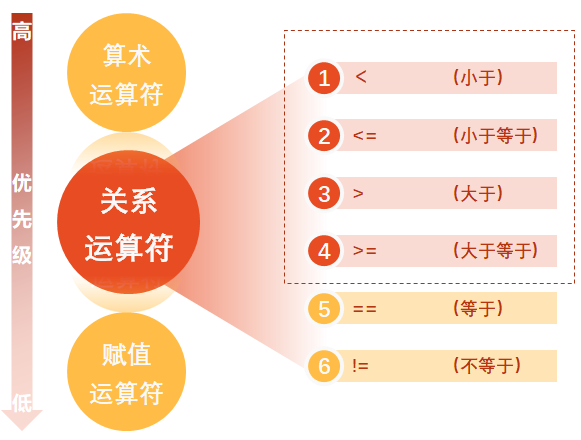
\includegraphics[scale=0.3]{pre}\\
分析:
\begin{lstlisting}
if(a>b==c){...}
if(a=b>c) {...}
\end{lstlisting}
\end{columns}
\end{frame}

\begin{frame}[shrink,fragile]{关系表达式的值, 非0即真}
\begin{block}{关系表达式}
	\small
	\begin{itemize}
		\item 用关系运算符将两个数值或数值表达式连接起来的式子,称为关系表达式。
		\item 关系表达式的值是一个逻辑值,即``真''或``假''。
		\item 在C的逻辑运算中, 以``1''代表``真'',以``0''代表``假''。	
	\end{itemize}
\end{block}
\begin{columns}[T]
\column{0.5\textwidth}
\begin{lstlisting}
int a=3, b=2, c=1, d1, d2; 
d1 = a > b; // d1=1
d2 = a > b > c; //自左至右结合,d2=0
if(d1)
{ printf("执行此语句") }
if(d2) 
{ printf("不执行此语句"); }
\end{lstlisting}
\column{0.5\textwidth}
\begin{lstlisting}
if(d1 = a > b) // d1的值就是表达式的值
{ printf("执行此语句"); }
if(d2 = a > b > c)//d2的值就是表达式的值
{ printf("不执行此语句"); }
\end{lstlisting}
\end{columns}
\end{frame}

\section{逻辑运算符}

\begin{frame}[shrink,fragile]{逻辑运算符}
\begin{lstlisting}
int a=5,b=10,c=0; //以int为例
if(!a) // 逻辑非(NOT), a是非0, 所以!a的值是0
{ ... }
if(a && b) // 逻辑与(AND), a,b均为非0, 所以(a && b)的值为1
{ ... }
if(a || c) // 逻辑或(OR), a,c之一是非0, 即为真
{ ... }
\end{lstlisting}
\end{frame}

\begin{frame}[shrink,fragile]{逻辑运算符真值表}
\begin{tabular}{|c|c||c|c|c|c|}
\hline 
a       & b      & !a    & !b    & a\&\&b & a||b \\ 
\hline 
真(非0) & 真(非0) & 假(0) & 假(0) & 真(1)  & 真(1) \\ 
\hline
真(非0) & 假(0)   & 假(0) & 真(1) & 假(0)  & 真(1) \\ 
\hline 
假(0)   & 真(非0) & 真(1) & 假(0) & 假(0)  & 真(1) \\ 
\hline 
假(0)   & 假(0)   & 真(1) & 真(1) & 假(0)  & 假(0) \\ 
\hline  
\end{tabular} 
\begin{itemize}
	\item ``\&\&''和``‖''是双目运算符,要求有两个运算对象(操作数);\\ ``!''是单目运算符,只要有一个运算对象
	\item 由高到低优先次序: !(非)$\to$\&\&(与)$\to$‖(或);\\
          逻辑运算符中的``\&\&''和``||''低于关系运算符, ``!''高于算术运算符
	\item 逻辑运算结果不是0就是1,不可能是其他数值。\\
	      而运算对象可以是0(假)或任何非0的数值(按``真''对待)
\end{itemize}
\end{frame}

\begin{frame}[shrink,fragile]{逻辑运算示例(1)}
判别用year表示的某一年是否闰年,可以用一个逻辑表达式来表示。闰年的条件是符合下面二者之一: (1)能被4整除,但不能被100整除。(2)能被100整除,又能被400整除。
\begin{lstlisting}
int year;
scanf("%d",&year);
\\ 闰年
if(year%4 == 0 && year%100 != 0)
{ printf("%d是闰年\n", year); }
else if(year%100 == 0 && year%400 == 0)
{ printf("%d是闰年\n", year); }
else
{ printf("%d不是闰年\n", year)}
\end{lstlisting}
\end{frame}

\begin{frame}[shrink,fragile]{逻辑运算示例(2)}
判别用year表示的某一年是否闰年,可以用一个逻辑表达式来表示。闰年的条件是符合下面二者之一: (1)能被4整除,但不能被100整除。(2)能被100整除,又能被400整除。
\begin{lstlisting}
int year, flag = 'N';
scanf("%d",&year);
\\ 闰年
if(year%4 == 0 && year%100 != 0)
{ flag = 'Y'; }
else
{ 
   if(year%100 == 0 && year%400 == 0)
   { flag = 'Y'; }
}
if(flag == 'Y') 
{ printf("%d是闰年\n", year); }
else
{ printf("%d不是闰年\n", year); }
\end{lstlisting}
\end{frame}

\begin{frame}[shrink,fragile]{逻辑运算示例(3)}
判别用year表示的某一年是否闰年,可以用一个逻辑表达式来表示。闰年的条件是符合下面二者之一: (1)能被4整除,但不能被100整除。(2)能被100整除,又能被400整除。
\begin{lstlisting}
int year;
scanf("%d",&year);
\\ 闰年
if((year%4 == 0 && year%100 != 0)||(year%100 == 0 && year%400 == 0))
{ printf("%d是闰年\n", year); }
else
{ printf("%d不是闰年\n", year)}
\end{lstlisting}
\end{frame}

\section{条件运算符和条件表达式}

\begin{frame}[shrink,fragile]{条件运算符和条件表达式}
\begin{columns}[T]
\column{0.5\textwidth}
\begin{lstlisting}
int a,b;
scanf("%d%d",&a,&b);
if(a>b)
{ max = a; }
else
{ max = b; }
// 等效为
max = (a>b) ? a : b;
// 或
a>b ? (max=a) : (max=b);
// 甚至用在语句中
printf("%d\n",a>b ? a : b);
\end{lstlisting}
\column{0.5\textwidth}
\colorbox{yellow}{\textcolor{blue}{表达式1 ? 表达式2 : 表达式3}}\\
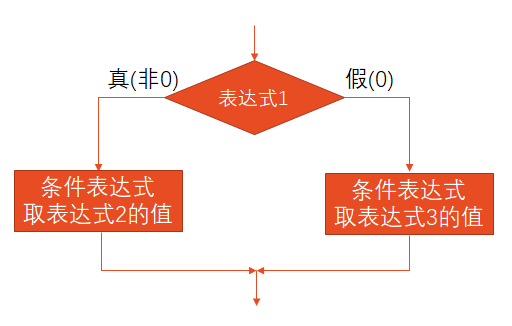
\includegraphics[scale=0.3]{if3}
\end{columns}
\end{frame}

\begin{frame}[shrink,fragile]{例: 大写转小写字母}
[例4.4, p96]输入一个字符, 判别它是否为大写字母, 如果是,将它转换成小写字母; 如果不是, 不转换。然后输出最后得到的字符。
\begin{lstlisting}
char ch;
scanf("%c",&ch);
ch = (ch>='A' && ch<='Z') ? (ch+32) : ch;
// 等效于
if(ch>='A' && ch<='Z')
{
   ch = ch+32; // 可简写为 ch += 32;
}
printf("ch=%c\n",ch);
\end{lstlisting}
\end{frame}

\section{数学表达式与C语言表达式的不同}

\begin{frame}[shrink,fragile]{数学表达式与C语言表达式的不同}
\begin{lstlisting}
int a = 10;
if(20 <= a && a <= 30) // 表达式的值为假(0)
{ ...  }
if(20 <= a <= 30) // 表达式为真(1)
{ ...  }
// 类似的
// if(a==20) 与 if(a=20)意义不同.
if(a==20) //表达式的值是假(0)
{ ... }
if(a=20) //表达式的值是10, 非0, 表示为真, 并且a被赋值为20
{ ... }
\end{lstlisting}
\end{frame}

\section{用switch语句实现多分支选择结构}

\begin{frame}[shrink,fragile]{用switch语句实现多分支选择结构}
switch(int或char型表达式)
\begin{columns}[T]
\column{0.5\textwidth}
\begin{lstlisting}
int a;
scanf("%d",&a)
swach(a)
{
   case 10: 多条语句1; 
            break;
   case 20: 多条语句2; 
            break;
   case 30: 多条语句3; 
            break;
   default: 多条语句4;
}
\end{lstlisting}
\column{0.5\textwidth}
\begin{lstlisting}
int a;
scanf("%d",&a)
if(a == 10)
{ 多条语句1; } 
else if(a == 20 )
{ 多条语句2; } 
else if(a == 30) 
{ 多条语句3; }
else
{ 多条语句4; }
\end{lstlisting}
\end{columns}
\end{frame}

\begin{frame}[shrink,fragile]
\begin{columns}[T]
\column{0.5\textwidth}
\begin{lstlisting}
char a; // 或 int a;
scanf("%c",&a)
swach(a)
{
    case 'A':
    case 'a': 多条语句1; 
              break;
    case 'B':
    case 'b': 多条语句2; 
              break;
    case 'C':
    case 'c': 多条语句3; 
              break;
    default: 多条语句4;
}
\end{lstlisting}
\column{0.5\textwidth}
\begin{lstlisting}	
char a; // 或 int a;
scanf("%d",&a)
if(a == 'A' || a == 'a')
{ 多条语句1; } 
else if(a == 'B' || a == 'b')
{ 多条语句2; } 
else if(a == 'C' || a == 'c') 
{ 多条语句3; }
else
{ 多条语句4; }
\end{lstlisting}
\end{columns}
\end{frame}

\begin{frame}[shrink,fragile]
\begin{columns}[T]
\column{0.4\textwidth}
\small
[例4.10,p99]运输公司对用户计算运输费用。路程越远,运费越低。标准如下:  
\begin{align*}
s<250 &&\text{没有折扣}\\
250\le s < 500 &&\text{2\%折扣}\\
500\le s < 1000 &&\text{5\%折扣}\\
1000\le s < 2000 &&\text{8\%折扣}\\
2000\le s < 3000 &&\text{10\%折扣}\\
3000\ge s  &&\text{15\%折扣}
\end{align*}
\column{0.6\textwidth}
\begin{lstlisting}
int c,s; //c是分类整数, s是距离
float p,w,d,f; //单价,重量,折扣,运费
// 运费 f = p*w*s*(1-d%) 
if(s>=3000) { c = 12; } else {c = s/250; }
switch(c) {
   case 0: d=0; break;
   case 1: d=2; break;
   case 2: case 3: d=5; break;
   case 4: case 5: case 6: case 7: 
        d=8; break;
   case 8: case 9: case 10: case 11: 
        d=10 break;
   case 12: d=15; break;
}
f = p*w*s*(1-d/100);  printf("%.2f\n",f);
\end{lstlisting}
\end{columns}
\end{frame}
 % 开发平台实例演示: 数据输入再讨论
%%%%%%%%%%%%%%%%%%%%%%%%%%% lecture-1
\begin{frame}[shrink]
  \frametitle{lecture-4 主要内容}
  \framesubtitle{选择结构程序设计}
  \tableofcontents[hideallsubsections]
\end{frame}

\section{选择结构和条件判断}

\begin{frame}{选择结构和条件判断}
\begin{columns}
	\column{0.6\textwidth}
	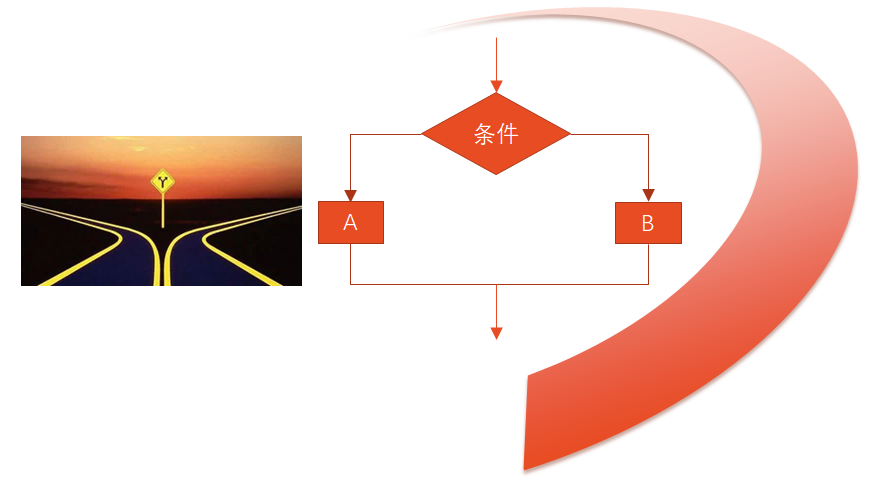
\includegraphics[scale=0.25]{if-case}
	\column{0.4\textwidth}
	\begin{block}{C语言有两种选择语句}
		\begin{itemize}
			\item if语句, 用来实现\textbf{两个分支}的选择结构
			\item switch语句, 用来实现\textbf{多分支}的选择结构
		\end{itemize}
	\end{block}
\end{columns}
\end{frame}

\begin{frame}[fragile]{if(条件表达式)\{ 表达式为真(非0)时执行语句; \}}
\begin{lstlisting}
#include<stdio.h>            // standard input/output编译预处理指令
int main()                   // 主函数
{                            // 函数开始标志
   int a=10;    // 定义变量a为整型数值, 定义变量时,可以指定变量的初值
   if(a>=10)
   {
      printf("a>=10\n"); // \n为换行符
   }
   else
   {
      printf("a<10\n"); // \n为换行符
   }
   return 0;                 // 函数执行完毕返回函数值0
}                            // 函数结束标志
\end{lstlisting}
\end{frame}

\begin{frame}[shrink,fragile]
\small [例4.1 p84] 求$ax^2+bx+c=0$方程的根。$a,b,c$由键盘输入。
\begin{lstlisting}
#include<stdio.h>
#include<math.h>   // 数学库函数        
int main()                   
{  
   double a,b,c,x1,x2,delta;
   scanf("%lf%lf%lf",&a,&b,&c);
   if(b*b-4*a*c < 0) 
   { printf("This equation hasn\'t real roots!\n"); }
   else
   {
      delta = sqrt(b*b-4*a*c);
      x1 = -b + delta/(2*a);  x2 = -b - delta/(2*a);
      printf("x1=%.2lf,x2=%.2lf\n",x1,x2);
   }
   return 0;           
}                            
\end{lstlisting}
\end{frame}

\begin{frame}[shrink,fragile]
\small [例4.2 p85] 输入两个实数, 按由小到大的顺序输出这两个数。
\begin{columns}
\column{0.45\textwidth}
\begin{lstlisting}
#include<stdio.h>        
int main()                   
{  
   float a,b,t;
   scanf("%f%f",&a,&b); 
   //不好: scanf("%f,%f",&a,&b);
   if(a>b)
   {  //将a和b的值互换
      t=a;
      a=b;
      b=t;
   }
   printf("%.2f,%.2f\n",a,b);
   return 0;           
}
\end{lstlisting} 
\column{0.55\textwidth}
\small
\begin{block}{两个变量值的互换}
a=b;  //把变量b的值赋给变量a,a的值等于b的值\\
b=a;  //再把变量a的值赋给变量b,变量b值没有改变
\end{block}
\textbf{因此, 为了实现互换, 必须借助于第三个变量。}
\end{columns}                           
\end{frame}

\begin{frame}[shrink,fragile]
\small [例4.3 p86] 输入3个数a, b, c, 要求按由小到大的顺序输出。
\begin{lstlisting}
#include<stdio.h>        
int main()                   
{  
    float a,b,c,t;
    scanf("%f%f%f",&a,&b,&c); //不好: scanf("%f,%f,%f",&a,&b,&c);
    if(a>b)
    {
       t=a; a=b; b=t; //借助变量t,实现变量a和变量b互换值
    } //互换后,a小于或等于b     
    if(a>c)
    {
       t=a; a=c; c=t; //借助变量t,实现变量a和变量c互换值
    } //互换后,a小于或等于c       
    if(b>c) //还要
    { 
       t=b; b=c; c=t; //借助变量t,实现变量b和变量c互换值
    }  //互换后,b小于或等于c                       
    printf("%.2f,%.2f,%.2f\n",a,b,c); //顺序输出a,b,c的值
    return 0;  
}
\end{lstlisting}                   
\end{frame}

\section{if语句的一般形式}

\begin{frame}[shrink,fragile]{if(条件表达式)\{ 表达式为真(非0)时执行语句; \}}
\textbf{条件表达式: 关系表达式; 逻辑表达式; 数值表达式。}
\begin{columns}[t]
\column{0.3\textwidth}
\begin{beamerboxesrounded}{形式1(无else)}
\begin{lstlisting}
// 形式1(无else)
if(条件表达式)
{
   多条语句(复合语句);
}
\end{lstlisting}
\end{beamerboxesrounded}
\column{0.3\textwidth}
\begin{beamerboxesrounded}{形式2}
\begin{lstlisting}
// 形式2
if(条件表达式)
{
   多条语句(复合语句);
}
else
{
   多条语句(复合语句);
}
\end{lstlisting} 
\end{beamerboxesrounded}
\column{0.4\textwidth}
\begin{beamerboxesrounded}{形式3(排除式)}
\begin{lstlisting}
// 形式3(排除式)
if(条件表达式1)
{
   多条语句(复合语句);
}
else if(条件表达式2)//可多个
{
   多条语句(复合语句);
}
else
{
   多条语句(复合语句);
}
\end{lstlisting}
\end{beamerboxesrounded}
\end{columns}                        
\end{frame}

\section{关系运算符及其优先次序}

\begin{frame}[shrink,fragile]{关系运算符及其优先次序}
\begin{columns}%[t]
\column{0.5\textwidth}
\begin{lstlisting}
int a=5,b=10,c=20; //以int为例
if(a<b+c) // 相当于a<(b+c)
{ ... }
if(a<=b+c) 
{ ... }
if(a>b+c) 
{ ... }
if(a>=b+c) 
{ ... }
if(a==b+c)//a是否等于(b+c),与a=(b+c)不同
{ ... }
if(a!=b+c) // a不能于(b+c)
{ ... }
\end{lstlisting}
\column{0.5\textwidth}
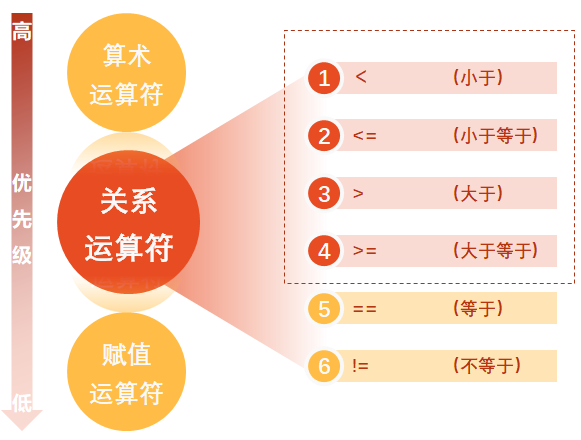
\includegraphics[scale=0.3]{pre}\\
分析:
\begin{lstlisting}
if(a>b==c){...}
if(a=b>c) {...}
\end{lstlisting}
\end{columns}
\end{frame}

\begin{frame}[shrink,fragile]{关系表达式的值, 非0即真}
\begin{block}{关系表达式}
	\small
	\begin{itemize}
		\item 用关系运算符将两个数值或数值表达式连接起来的式子,称为关系表达式。
		\item 关系表达式的值是一个逻辑值,即``真''或``假''。
		\item 在C的逻辑运算中, 以``1''代表``真'',以``0''代表``假''。	
	\end{itemize}
\end{block}
\begin{columns}[T]
\column{0.5\textwidth}
\begin{lstlisting}
int a=3, b=2, c=1, d1, d2; 
d1 = a > b; // d1=1
d2 = a > b > c; //自左至右结合,d2=0
if(d1)
{ printf("执行此语句") }
if(d2) 
{ printf("不执行此语句"); }
\end{lstlisting}
\column{0.5\textwidth}
\begin{lstlisting}
if(d1 = a > b) // d1的值就是表达式的值
{ printf("执行此语句"); }
if(d2 = a > b > c)//d2的值就是表达式的值
{ printf("不执行此语句"); }
\end{lstlisting}
\end{columns}
\end{frame}

\section{逻辑运算符}

\begin{frame}[shrink,fragile]{逻辑运算符}
\begin{lstlisting}
int a=5,b=10,c=0; //以int为例
if(!a) // 逻辑非(NOT), a是非0, 所以!a的值是0
{ ... }
if(a && b) // 逻辑与(AND), a,b均为非0, 所以(a && b)的值为1
{ ... }
if(a || c) // 逻辑或(OR), a,c之一是非0, 即为真
{ ... }
\end{lstlisting}
\end{frame}

\begin{frame}[shrink,fragile]{逻辑运算符真值表}
\begin{tabular}{|c|c||c|c|c|c|}
\hline 
a       & b      & !a    & !b    & a\&\&b & a||b \\ 
\hline 
真(非0) & 真(非0) & 假(0) & 假(0) & 真(1)  & 真(1) \\ 
\hline
真(非0) & 假(0)   & 假(0) & 真(1) & 假(0)  & 真(1) \\ 
\hline 
假(0)   & 真(非0) & 真(1) & 假(0) & 假(0)  & 真(1) \\ 
\hline 
假(0)   & 假(0)   & 真(1) & 真(1) & 假(0)  & 假(0) \\ 
\hline  
\end{tabular} 
\begin{itemize}
	\item ``\&\&''和``‖''是双目运算符,要求有两个运算对象(操作数);\\ ``!''是单目运算符,只要有一个运算对象
	\item 由高到低优先次序: !(非)$\to$\&\&(与)$\to$‖(或);\\
          逻辑运算符中的``\&\&''和``||''低于关系运算符, ``!''高于算术运算符
	\item 逻辑运算结果不是0就是1,不可能是其他数值。\\
	      而运算对象可以是0(假)或任何非0的数值(按``真''对待)
\end{itemize}
\end{frame}

\begin{frame}[shrink,fragile]{逻辑运算示例(1)}
判别用year表示的某一年是否闰年,可以用一个逻辑表达式来表示。闰年的条件是符合下面二者之一: (1)能被4整除,但不能被100整除。(2)能被100整除,又能被400整除。
\begin{lstlisting}
int year;
scanf("%d",&year);
\\ 闰年
if(year%4 == 0 && year%100 != 0)
{ printf("%d是闰年\n", year); }
else if(year%100 == 0 && year%400 == 0)
{ printf("%d是闰年\n", year); }
else
{ printf("%d不是闰年\n", year)}
\end{lstlisting}
\end{frame}

\begin{frame}[shrink,fragile]{逻辑运算示例(2)}
判别用year表示的某一年是否闰年,可以用一个逻辑表达式来表示。闰年的条件是符合下面二者之一: (1)能被4整除,但不能被100整除。(2)能被100整除,又能被400整除。
\begin{lstlisting}
int year, flag = 'N';
scanf("%d",&year);
\\ 闰年
if(year%4 == 0 && year%100 != 0)
{ flag = 'Y'; }
else
{ 
   if(year%100 == 0 && year%400 == 0)
   { flag = 'Y'; }
}
if(flag == 'Y') 
{ printf("%d是闰年\n", year); }
else
{ printf("%d不是闰年\n", year); }
\end{lstlisting}
\end{frame}

\begin{frame}[shrink,fragile]{逻辑运算示例(3)}
判别用year表示的某一年是否闰年,可以用一个逻辑表达式来表示。闰年的条件是符合下面二者之一: (1)能被4整除,但不能被100整除。(2)能被100整除,又能被400整除。
\begin{lstlisting}
int year;
scanf("%d",&year);
\\ 闰年
if((year%4 == 0 && year%100 != 0)||(year%100 == 0 && year%400 == 0))
{ printf("%d是闰年\n", year); }
else
{ printf("%d不是闰年\n", year)}
\end{lstlisting}
\end{frame}

\section{条件运算符和条件表达式}

\begin{frame}[shrink,fragile]{条件运算符和条件表达式}
\begin{columns}[T]
\column{0.5\textwidth}
\begin{lstlisting}
int a,b;
scanf("%d%d",&a,&b);
if(a>b)
{ max = a; }
else
{ max = b; }
// 等效为
max = (a>b) ? a : b;
// 或
a>b ? (max=a) : (max=b);
// 甚至用在语句中
printf("%d\n",a>b ? a : b);
\end{lstlisting}
\column{0.5\textwidth}
\colorbox{yellow}{\textcolor{blue}{表达式1 ? 表达式2 : 表达式3}}\\
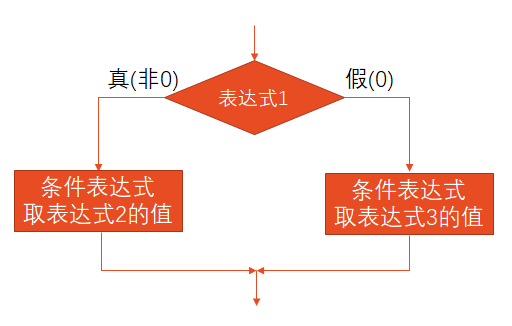
\includegraphics[scale=0.3]{if3}
\end{columns}
\end{frame}

\begin{frame}[shrink,fragile]{例: 大写转小写字母}
[例4.4, p96]输入一个字符, 判别它是否为大写字母, 如果是,将它转换成小写字母; 如果不是, 不转换。然后输出最后得到的字符。
\begin{lstlisting}
char ch;
scanf("%c",&ch);
ch = (ch>='A' && ch<='Z') ? (ch+32) : ch;
// 等效于
if(ch>='A' && ch<='Z')
{
   ch = ch+32; // 可简写为 ch += 32;
}
printf("ch=%c\n",ch);
\end{lstlisting}
\end{frame}

\section{数学表达式与C语言表达式的不同}

\begin{frame}[shrink,fragile]{数学表达式与C语言表达式的不同}
\begin{lstlisting}
int a = 10;
if(20 <= a && a <= 30) // 表达式的值为假(0)
{ ...  }
if(20 <= a <= 30) // 表达式为真(1)
{ ...  }
// 类似的
// if(a==20) 与 if(a=20)意义不同.
if(a==20) //表达式的值是假(0)
{ ... }
if(a=20) //表达式的值是10, 非0, 表示为真, 并且a被赋值为20
{ ... }
\end{lstlisting}
\end{frame}

\section{用switch语句实现多分支选择结构}

\begin{frame}[shrink,fragile]{用switch语句实现多分支选择结构}
switch(int或char型表达式)
\begin{columns}[T]
\column{0.5\textwidth}
\begin{lstlisting}
int a;
scanf("%d",&a)
swach(a)
{
   case 10: 多条语句1; 
            break;
   case 20: 多条语句2; 
            break;
   case 30: 多条语句3; 
            break;
   default: 多条语句4;
}
\end{lstlisting}
\column{0.5\textwidth}
\begin{lstlisting}
int a;
scanf("%d",&a)
if(a == 10)
{ 多条语句1; } 
else if(a == 20 )
{ 多条语句2; } 
else if(a == 30) 
{ 多条语句3; }
else
{ 多条语句4; }
\end{lstlisting}
\end{columns}
\end{frame}

\begin{frame}[shrink,fragile]
\begin{columns}[T]
\column{0.5\textwidth}
\begin{lstlisting}
char a; // 或 int a;
scanf("%c",&a)
swach(a)
{
    case 'A':
    case 'a': 多条语句1; 
              break;
    case 'B':
    case 'b': 多条语句2; 
              break;
    case 'C':
    case 'c': 多条语句3; 
              break;
    default: 多条语句4;
}
\end{lstlisting}
\column{0.5\textwidth}
\begin{lstlisting}	
char a; // 或 int a;
scanf("%d",&a)
if(a == 'A' || a == 'a')
{ 多条语句1; } 
else if(a == 'B' || a == 'b')
{ 多条语句2; } 
else if(a == 'C' || a == 'c') 
{ 多条语句3; }
else
{ 多条语句4; }
\end{lstlisting}
\end{columns}
\end{frame}

\begin{frame}[shrink,fragile]
\begin{columns}[T]
\column{0.4\textwidth}
\small
[例4.10,p99]运输公司对用户计算运输费用。路程越远,运费越低。标准如下:  
\begin{align*}
s<250 &&\text{没有折扣}\\
250\le s < 500 &&\text{2\%折扣}\\
500\le s < 1000 &&\text{5\%折扣}\\
1000\le s < 2000 &&\text{8\%折扣}\\
2000\le s < 3000 &&\text{10\%折扣}\\
3000\ge s  &&\text{15\%折扣}
\end{align*}
\column{0.6\textwidth}
\begin{lstlisting}
int c,s; //c是分类整数, s是距离
float p,w,d,f; //单价,重量,折扣,运费
// 运费 f = p*w*s*(1-d%) 
if(s>=3000) { c = 12; } else {c = s/250; }
switch(c) {
   case 0: d=0; break;
   case 1: d=2; break;
   case 2: case 3: d=5; break;
   case 4: case 5: case 6: case 7: 
        d=8; break;
   case 8: case 9: case 10: case 11: 
        d=10 break;
   case 12: d=15; break;
}
f = p*w*s*(1-d/100);  printf("%.2f\n",f);
\end{lstlisting}
\end{columns}
\end{frame}
 % 数据类型, 运算符和表达式, 数学库函数,顺序程序设计举例
%%%%%%%%%%%%%%%%%%%%%%%%%%% lecture-6
%\begin{frame}[shrink]
%  \frametitle{lecture-6 主要内容}
%  \framesubtitle{循环结构程序设计}
%  \tableofcontents[hideallsubsections]
%  %\tableofcontents[currentsection,hideallsubsections]
%\end{frame}

\begin{frame}[shrink,fragile]{为什么需要循环控制}
\begin{itemize}
	\item 要向计算机输入全班50个学生的成绩;(重复50次相同的输入操作)
	\item 分别统计全班50个学生的平均成绩;	(重复50次相同的计算操作)
\end{itemize}
\begin{lstlisting}[frame=lines]
float score1,score2,score3,score4,score5,aver; // 5门课成绩及平均成绩
// 输入第1个学生5门课的成绩
scanf(″%f%f%f%f%f″,&score1,&score2,&score3,&score4,&score5);
// 求第1个学生平均成绩
aver=(score1+score2+score3+score4+score5)/5;
printf(″aver=%7.2f″,aver); // 输出第1个学生平均成绩
// 输入第2个学生5门课的成绩
scanf(″%f%f%f%f%f″,&score1,&score2,&score3,&score4,&score5);
// 求第2个学生平均成绩
aver=(score1+score2+score3+score4+score5)/5;
printf(″aver=%7.2f″,aver);// 输出第2个学生平均成绩
...
\end{lstlisting}
\end{frame}

\begin{frame}[shrink,fragile]{用循环控制处理重复操作}
\begin{itemize}
	\item 要向计算机输入全班50个学生的成绩;(重复50次相同的输入操作)
	\item 分别统计全班50个学生的平均成绩;	(重复50次相同的计算操作)
\end{itemize}
\begin{lstlisting}[frame=lines]
float score1,score2,score3,score4,score5,aver; // 5门课成绩及平均成绩
int i=1;         // 设整型变量i初值为1   
while( i<=50 )   // 当i的值小于或等于50时执行花括号内的语句
{
   scanf("%f%f%f%f%f",&score1,&score2,&score3,&score4,&score5);
   aver=(score1+score2+score3+score4+score5)/5; 
   printf("aver=%7.2f",aver);
   i++;  // 每执行完一次循环使i的值加1 
}   
\end{lstlisting}
\end{frame}

\section{$while(\text{表达式})\{ \cdots\}$}

\begin{frame}[shrink,fragile]{$while(\text{表达式})\{ \cdots\}$}
\vspace{-0.5cm}
\begin{columns}[T]
	\column{0.25\textwidth}
	\begin{lstlisting} 
    while(表达式)   
    {
       // 循环体
       执行多条语句;  
    }   
    \end{lstlisting}
	\column{0.3\textwidth}
	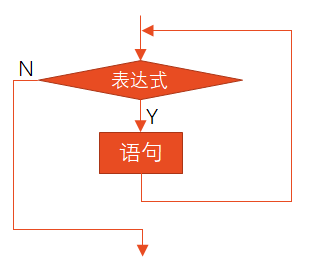
\includegraphics[scale=0.35]{while}
	\column{0.4\textwidth}
	\small
	\begin{block}{while循环特点}
		\small
		每轮循环: 首先判断表达式的值, 若``真" (以非0值表示)时,就执行循环体语句;为``假" (以0表示)时,就不执行循环体语句。
	\end{block}
\end{columns}
\vspace{-0.5cm}
\begin{columns}
\column{0.45\textwidth}
\begin{block}{常见错误}
\begin{lstlisting} 
while(表达式); 
{
   // 循环体
   执行多条语句;    
}
\end{lstlisting}
\end{block}
\column{0.45\textwidth}
\begin{block}{变体}
\begin{lstlisting} 
while(1)  
{
  if(表达式) break; // 退出循环
  执行多条语句;    
}
\end{lstlisting}
\end{block}
\end{columns}
\end{frame}

\begin{frame}[shrink,fragile]
$[$例5.1$]$ 求$1+2+3+\cdots+100$, 即$\sum\limits_{i=1}^{100}i$
\medskip
\begin{lstlisting}[frame=lines]
   int i=1,sum=0;      //定义变量i的初值为1,sum的初值为0  
   while(i <= 100)     //当i>100,条件表达式i<=100的值为假,不执行循环体
   {                   //循环体开始
      sum=sum+i;          //第1次累加后,sum的值为1
      i++;                //加完后,i的值加1,为下次累加做准备
   }                   //循环体结束
   printf("sum=%d\n",sum); //输出1+2+3…+100的累加和                
\end{lstlisting}
\begin{enumerate}
	\setlength{\itemsep}{.2cm}
	\item 循环体如果包含一个以上的语句,应该用花括号括起来,作为复合语句出现。
	\item 不要忽略给$i$和$sum$赋初值,否则它们的值是不可预测的,结果显然不正确。
	\item 在循环体中应有使循环趋向于结束的语句。如本例中的$i++;$语句。如果无此语句,则i的值始终不改变,循环永远不结束。
\end{enumerate}
\end{frame}

\section{$do \{\cdots\} while(\text{表达式});$}

\begin{frame}[shrink,fragile]{$do \{\cdots\} while(\text{表达式});$}
\vspace{-0.4cm}
\begin{columns}
	\column{0.3\textwidth}
	\begin{lstlisting} 
    do  
    {
      // 循环体
      执行多条语句;  
    } while( 表达式 );  
    \end{lstlisting}
	\column{0.3\textwidth}
	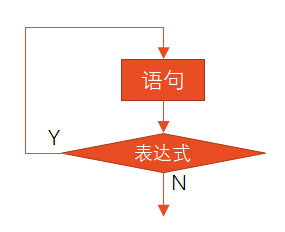
\includegraphics[scale=0.3]{dowhile}
	\column{0.35\textwidth}
	\begin{block}{循环特点}
		先无条件地执行循环体,然后判断循环条件是否成立。
	\end{block}
\end{columns}
\vspace{-0.5cm}
\begin{columns}
\column{0.45\textwidth}
\begin{block}{易犯错误}
\begin{lstlisting} 
do  
{
   // 循环体
   执行多条语句;  
} while( 表达式 )
\end{lstlisting}
\end{block}
\column{0.45\textwidth}
\begin{block}{变体}
\begin{lstlisting} 
do  
{
  执行多条语句;  
  if(表达式) break; // 退出循环  
} while(1);
\end{lstlisting}
\end{block}
\end{columns}
\end{frame}

\begin{frame}[shrink,fragile]
$[$例5.2$]$ 求$1+2+3+\cdots+100$, 即$\sum\limits_{i=1}^{100}i$
\medskip
\begin{lstlisting}[frame=lines]
int i=1,sum=0;      //定义变量i的初值为1,sum的初值为0  
do     
{                   //循环体开始
   sum=sum+i;          //第1次累加后,sum的值为1
   i++;                //加完后,i的值加1,为下次累加做准备
}while(i <= 100);   //当i>100,条件表达式i<=100的值为假,不执行循环体
printf("sum=%d\n",sum); //输出1+2+3…+100的累加和                
\end{lstlisting}
\begin{enumerate}
	\setlength{\itemsep}{.2cm}
	\item 在一般情况下,用while()\{$\cdots$\}语句和用do\{$\cdots$\}while();语句处理同一问题时,若二者的循环体部分是一样的,那么结果也一样。
	\item 但是如果while后面的表达式一开始就为假(0值)时,两种循环的结果是不同的。
\end{enumerate}
\end{frame}

\begin{frame}[shrink,fragile]{$while(\text{表达式})\{ \cdots\}$与$do \{\cdots\} while(\text{表达式});$}
$[$例5.3$]$ 求$\sum\limits_{i=n}^{100}i$。考虑输入$n>100$时的情况,以下程序的不同。
\begin{columns}
\column{0.4\textwidth}
\begin{lstlisting}[frame=single]
int i,sum=0;
scanf("%d",&i);      
while(i <= 100)     
{                   
  sum=sum+i;          
  i++;               
}                  
printf("sum=%d\n",sum);               
\end{lstlisting}
\column{0.4\textwidth}
\begin{lstlisting}[frame=single]
int i,sum=0;
scanf("%d",&i); 
do     
{                   
  sum=sum+i;          
  i++;                
}while(i <= 100);   
printf("sum=%d\n",sum);                
\end{lstlisting}
\end{columns}
\end{frame}

\section{$for(\text{表达式1;表达式2;表达式3}) \{\cdots\}$}

\begin{frame}[shrink,fragile]{$for(\text{表达式1;表达式2;表达式3}) \{\cdots\}$}
\vspace{-0.4cm}
\begin{columns}
\column{0.4\textwidth}
\begin{lstlisting}[frame=single] 
for(表达式1;表达式2;表达式3)
{
   // 循环体
   执行多条语句;  
}
\end{lstlisting}
$\equiv$
\begin{lstlisting}[frame=single] 
表达式1;
while(表达式2)
{
   // 循环体
   执行多条语句;
   表达式3;  
}
\end{lstlisting}
\column{0.4\textwidth}
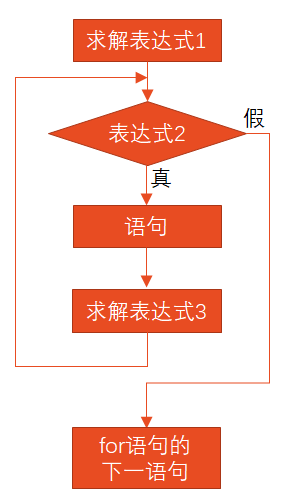
\includegraphics[scale=0.35]{for}
\end{columns}
\end{frame}

\begin{frame}[shrink,fragile]{$for(\text{表达式1;表达式2;表达式3}) \{\cdots\}$}
\begin{columns}
\column{0.25\textwidth}
\begin{lstlisting}[frame=single] 
for(表达式1;表达式2;表达式3)
{
   // 循环体
   执行多条语句;  
}
\end{lstlisting}
\column{0.3\textwidth}
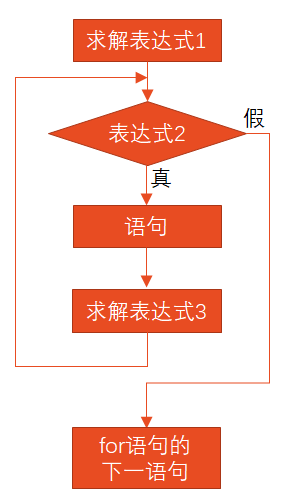
\includegraphics[scale=0.35]{for}
\column{0.45\textwidth}
\begin{itemize}
\item 表达式1: 设置初始条件,只执行一次。可以为零个、一个或多个变量(逗号隔开)设置初值。
\item 表达式2: 是循环条件表达式,用来判定是否继续循环。在每次执行循环体前先执行此表达式(包括第1次循环),决定是否继续执行循环。
\item 表达式3: 作为循环的调整,例如使循环变量增值,它是在执行完循环体后才进行的。	
\end{itemize}
\end{columns}
\end{frame}

\begin{frame}[shrink,fragile]{$for(\text{表达式1;表达式2;表达式3}) \{\cdots\}$, 省略表达式}
\vspace{-0.5cm}
\begin{columns}%[T]
\column{0.3\textwidth}
\begin{lstlisting} 
int i;
for(i=0;i<=100;i++)
{
  printf("%d\n",i);
}
\end{lstlisting}
\column{0.3\textwidth}
\begin{lstlisting}[frame=leftline] 
int i=0;
for(;i<=100;i++)
{
  printf("%d\n",i);
}
\end{lstlisting}
\column{0.4\textwidth}
\begin{lstlisting}[frame=leftline]
int i=0;
for(i=0;;i++)
{
  if(i>100) break;//退出循环
  printf("%d\n",i);
}
\end{lstlisting}
\end{columns}
\rule{\textwidth}{1pt} % 水平线
\begin{columns}%[T]
\column{0.3\textwidth}
\begin{lstlisting} 
int i;
for(i=0;i<=100;)
{
  printf("%d\n",i);
  i++;
}
\end{lstlisting}
\column{0.3\textwidth}
\begin{lstlisting}[frame=leftline] 
int i=0;
for(;i<=100;)
{
  printf("%d\n",i);
  i++;
}
\end{lstlisting}
\column{0.4\textwidth}
\begin{lstlisting}[frame=leftline] 
int i=0;
for(;;)
{
  if(i>100) break;//退出循环  
  printf("%d\n",i);
  i++
}
\end{lstlisting}
\end{columns}
\end{frame}

\section{循环的嵌套}

\begin{frame}{循环的嵌套}
\centering
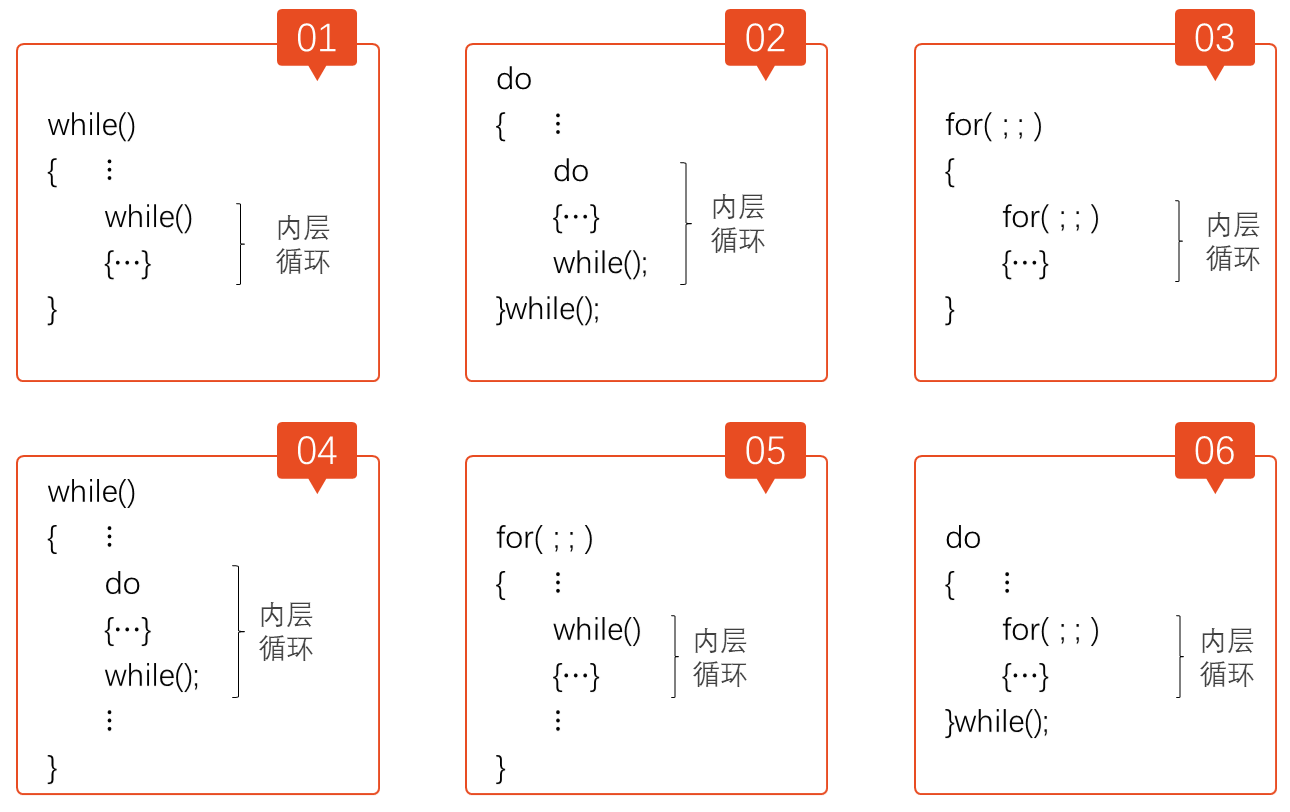
\includegraphics[scale=0.24]{whileWhile}
\end{frame}

\begin{frame}{几种循环的比较}
\begin{enumerate}
	\item 3种循环都可以用来处理同一问题,一般情况下它们可以互相代替。
	\item 在while循环和do…while循环中,只在while后面的括号内指定循环条件,因此为了使循环能正常结束,应在循环体中包含\textbf{使循环趋于结束的语句}(如i++等)。
	\item for循环可以在表达式3中包含使循环趋于结束的操作,甚至可以将循环体中的操作全部放到表达式3中(逗号隔开)。因此for语句的功能更强,凡用while循环能完成的,用for循环都能实现。
	\item 用while和do…while循环时,循环变量初始化的操作应在while和do…while语句之前完成。而for语句可以在表达式1中实现循环变量的初始化。
	\item while循环、do…while循环和for循环都可以用break语句跳出循环,用continue语句结束本次循环。	
\end{enumerate}
\end{frame}

\section{break,continue改变循环执行的状态}

\begin{frame}[shrink,fragile]{break,continue改变循环执行的状态}
\centering
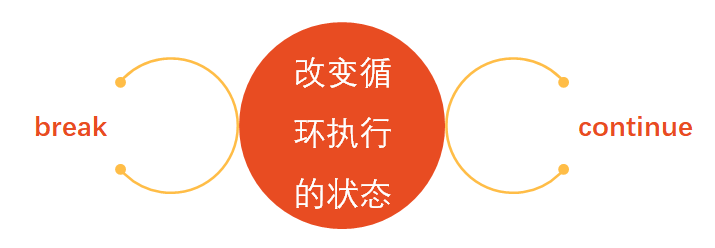
\includegraphics[scale=0.3]{breakContinue}
\begin{columns}[T]
\column{0.5\textwidth}
\begin{lstlisting}
while(表达式)
{
  printf("语句1");
  if(条件表达式) break; //提前终止循环
  printf("语句1");
}
\end{lstlisting}
\column{0.5\textwidth}
\begin{lstlisting}[frame=leftline]
while(表达式)
{
   printf("语句1");
   if(条件表达式) continue; //结束本次循环, 进入下轮循环
   printf("语句1");
}
\end{lstlisting}
\end{columns}
\end{frame}

\begin{frame}[shrink,fragile]{用break语句提前终止循环}
$[$例5.4$]$在全系1000名学生中举行慈善募捐,当总数达到10万元时就结束,统计此时捐款的人数以及平均每人捐款的数目。
\begin{lstlisting}
#define SUM 100000  //指定符号常量SUM代表10万
float amount,aver,total; 
int i;
for (i=1,total=0; i<=1000; i++)// 表达式1给多个变量赋初值,用逗号隔开。
{
  printf("please enter amount:");
  scanf("%f",&amount);
  total = total + amount; 
  if(total >= SUM) break; // 终止整个循环,也不会执行for语句的表达式3 (i++)
}
aver=total/i;
printf("num=%d\naver=%10.2f\n",i,aver); 
\end{lstlisting}
\textbf{\textcolor{blue}{注意: break语句只能用于循环语句和switch语句之中,而不能单独使用。}}
\end{frame}

\begin{frame}[shrink,fragile]{用continue语句提前结束本次循环}
$[$例5.4$]$要求输出100$\sim$200之间的不能被3整除的数。
\vspace{-0.3cm}
\begin{columns}
\column{0.75\textwidth}
\begin{lstlisting}
#include <stdio.h>
int main()
{
  int n;
  for (n = 100;n <= 200;n++)
  {
    //终止本轮循环,但会执行for语句的表达式3(n++),开始下轮循环
    if (n%3==0) continue;
    printf("%d ",n);
  }
  printf("\n");
  return 0;
} 
\end{lstlisting}
\column{0.25\textwidth}
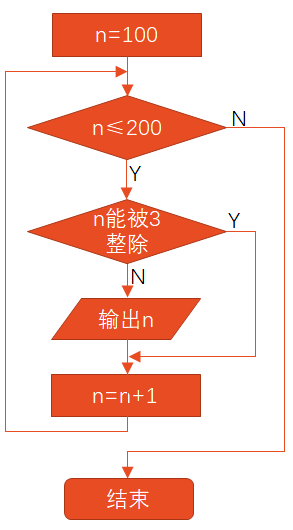
\includegraphics[scale=0.3]{for3}
\end{columns}
\end{frame}

\begin{frame}{break语句和continue语句的区别}
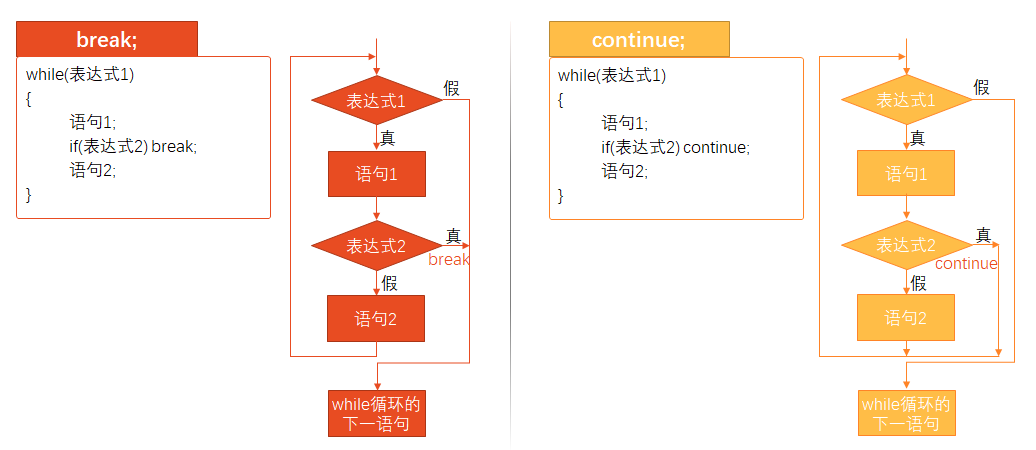
\includegraphics[scale=0.34]{forContinue}\\
\textbf{\textcolor{blue}{注意: continue语句只结束本次循环,而非终止整个循环。break语句结束整个循环,不再判断执行循环的条件是否成立。}}
\end{frame}

\begin{frame}[shrink,fragile]{break语句和continue语句的区别}
\small $[$例5.5$]$ 输出以下$4\times 5$的矩阵。
\vspace{-0.5cm}
\begin{columns}
\column{0.5\textwidth}
\begin{lstlisting}
int i,j,n=0;
for(i=1;i<=4;i++)
{
  for(j=1;j<=5;j++,n++) //n用来累计输出数据的个数
  {
    if(n%5==0) printf("\n"); //控制在输出5个数据后换行
    if (i==3 && j==1) break;
    printf("%d\t",i*j);
  } 
} 
printf("\n");  
\end{lstlisting}
\column{0.5\textwidth}
\vspace{-0.3cm}
\begin{lstlisting}[frame=leftline]
int i,j,n=0;
for(i=1;i<=4;i++)
{
   for(j=1;j<=5;j++,n++) //n用来累计输出数据的个数
   {
     if(n%5==0) printf("\n"); //控制在输出5个数据后换行
     if (i==3 && j==1) continue;
     printf("%d\t",i*j); // \t就是Tab键,是特殊字符,表示多个空格
   } 
} 
printf("\n");    
\end{lstlisting}
\end{columns}
\end{frame}

\begin{frame}[fragile]{分析下列程序片段, 体会break与continue的不同}
\vspace{-0.5cm}
\begin{columns}
\column{0.52\textwidth}
\begin{lstlisting}
int i=0;
while(i<4)
{
  if(i==2) 
  {
    i++;
    continue;//终止本轮循环,开始下轮循环 
  }
  printf("i=%d,",i);//i=0,i=1,i=3,
  i++;
}
printf("\nend i=%d\n",i);//end i=4
\end{lstlisting} 
\column{0.48\textwidth}
\begin{lstlisting}[frame=leftline]
int i=0;
while(i<4)
{
  if(i==2) 
  {
    i++;
    break; // 终止整个循环 
  }
  printf("i=%d,",i);//i=0, i=1, 
  i++;
}
printf("\nend i=%d\n",i);//end i=3 
\end{lstlisting} 
\end{columns}
\end{frame}

\begin{frame}[fragile]{分析下列程序片段, 体会break与continue的不同}
\vspace{-0.5cm}
\begin{columns}
\column{0.52\textwidth}
\begin{lstlisting}
int i=0;
for(i=0;i<4;i++) //对于continue语句, 表达式3是本轮循环的一部分 
{
  if(i==2) continue; //终止本轮循环,但会执行for语句的表达式3 (i++), 开始下轮循环 
  printf("i=%d,",i); //i=0,i=1,i=3,
}
printf("\nend i=%d\n",i);
//end i=4
\end{lstlisting} 
\column{0.48\textwidth}
\begin{lstlisting}[frame=leftline]
int i=0;
for(i=0;i<4;i++) //对于break语句, 终止整个循环, 表达式3也不会执行 
{
  if(i==2) break; //终止整个循环,也不会执行for语句的表达式3 (i++)
  printf("i=%d,",i); // i=0,i=1, 
}
printf("\nend i=%d\n",i);
//end i=2, 此处根据循环变量i的值可以判断上述循环是否正常结束, if(i==4) 正常结束。 
\end{lstlisting} 
\end{columns}
\end{frame}

\begin{frame}{注意事项小结}
\begin{enumerate}
	\setlength{\itemsep}{.5cm}
	\item while( )\{ \}; do \{ \} while( ); for(;;)\{ \}执行顺序;
	\item 循环变量的开始和结束条件;
	\item 循环体是复合语句时,必须用\{ \}扩起来;
	\item 必要时,用break结束整个循环,用continue结束本次循环;
	\item 关键是找出循环规律,必要时设计流程图,指导代码实现。	
\end{enumerate}
\end{frame} % ch4, 选择结构程序设计
%%%%%%%%%%%%%%%%%%%%%%%%%%% lecture-7
%\begin{frame}[shrink]
%  \frametitle{lecture-7 主要内容}
%  \framesubtitle{循环结构程序设计举例}
%  \tableofcontents[hideallsubsections]
%\end{frame}

\section{循环结构程序设计举例}

\begin{frame}[shrink,fragile]
$[$例5.7$]$用公式$\frac{\pi}{4}\approx 1-\frac{1}{3}+\frac{1}{5}-\frac{1}{7}+\cdots$求$\pi$的近似值, 直到发现某一项的绝对值小于$10^{-6}$为止(该项不累加)。\\
~\\
\begin{columns}
\column{0.7\textwidth}
解题思路:  找规律
\begin{enumerate}
	\item 每项的分子都是1。
	\item 后一项的分母是前一项的分母加2。
	\item 第1项的符号为正,从第2项起,每一项的符号与前一项的符号相反。
	在每求出一项后,检查它的绝对值是否大于或等于$10^{-6}$。
\end{enumerate}
\column{0.3\textwidth}
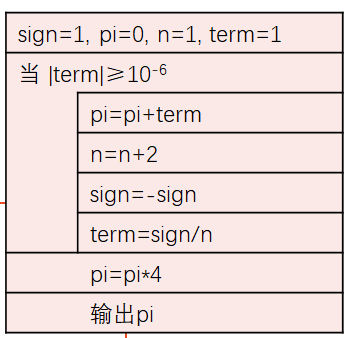
\includegraphics[scale=0.3]{pi}
\end{columns}
\end{frame}

\begin{frame}[shrink,fragile]
\begin{lstlisting}
#include <stdio.h>
#include <math.h> //程序中用到数学函数fabs,应包含头文件math.h
int main()
{
  int sign=1; //sign用来表示数值的符号
  double pi=0.0,n=1.0,term=1.0; //pi开始代表多项式的值,最后代表π的值, n代表分母,term代表当前项的值
  while(fabs(term)>=1e-6) //检查当前项term的绝对值是否大于或等于$10^{-6}$
  {
    pi=pi+term; //把当前项term累加到pi中
    n=n+2;      //n+2是下一项的分母 
    sign=-sign; //sign代表符号,下一项的符号与上一项符号相反
    term=sign/n; //求出下一项的值term
  }
  pi=pi*4; //多项式的和pi乘以4,才是$\pi$的近似值
  printf("pi=%10.8f\n",pi);  //输出$\pi$的近似值  
  return 0;
}
\end{lstlisting}
\end{frame}

\begin{frame}[shrink,fragile]
\small
$[$例5.8$]$求Fibonacci(斐波那契)数列的前40个数。这个数列有如下特点: 第1, 2两个数为1, 1。从第3个数开始,该数是其前面两个数之和。即该数列为1,1,2,3,5,8,13,\dots,用数学方式表示为:
\[
\begin{cases}
F_1=1 & (n=1)\\
F_2=1 & (n=2)\\
F_n=F_{n-1}+F_{n-2} & (n\ge 3)\\
\end{cases}
\]
\begin{columns}
	\column{0.4\textwidth}
	这是一个有趣的古典数学问题: 有一对兔子,从出生后第3个月起每个月都生一对兔子。小兔子长到第3个月后每个月又生一对兔子。假设所有兔子都不死,问每个月的兔子总数为多少?
	\column{0.6\textwidth}
	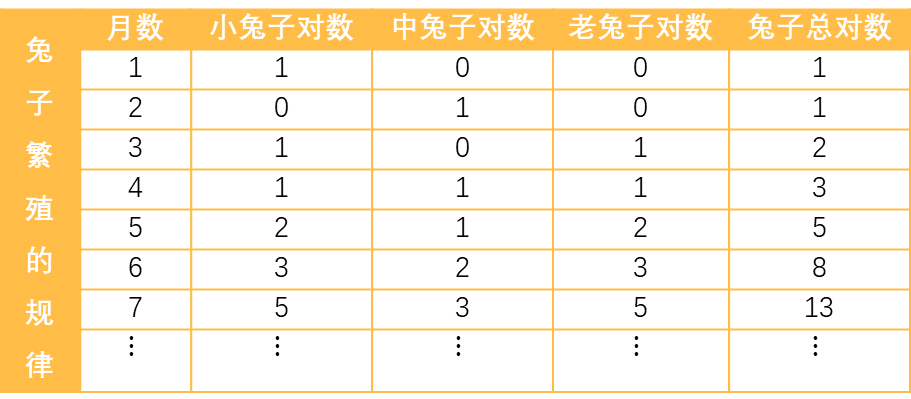
\includegraphics[scale=0.45]{Fn}
	\scriptsize
	不满1个月的为小兔子,满1个月不满2个月的为中兔子,满2个月以上的为老兔子。
\end{columns}
\end{frame}

\begin{frame}[shrink,fragile]
解法一: 利用递推(迭代)公式: $F_1=F_2=1; F_3=F_1+F_2; F_1=F_2; F_2=F_3; $
\begin{columns}
	\column{0.6\textwidth}
	\begin{lstlisting}
    #include <stdio.h>
    int main()
    {
        int f1=1,f2=1,f3;
        int i;
        printf("%12d\n%12d\n",f1,f2);
        for(i=1; i<=38; i++)
        {
            f3=f1+f2;
            printf("%12d\n",f3);
            f1=f2;
            f2=f3;
        }
        return 0;
    }
    \end{lstlisting}
	\column{0.3\textwidth}
	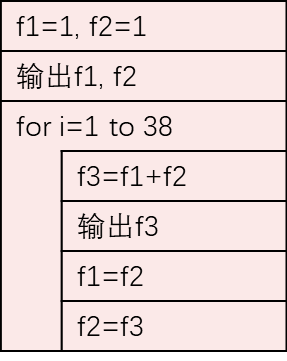
\includegraphics[scale=0.6]{Fn1}\\
	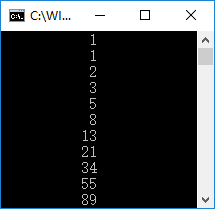
\includegraphics[scale=0.6]{Fno1}
\end{columns}
\end{frame}

\begin{frame}[shrink,fragile]
解法二: 利用递推(迭代)公式: $F_1=F_2=1; F_1=F_1+F_2; F_2=F_1+F_2; $
\begin{columns}
	\column{0.5\textwidth}
\begin{lstlisting}
#include <stdio.h>
int main()
{
  int f1=1,f2=1;
  int i;
  for(i=1; i<=20; i++)
  {
    printf("%12d%12d",f1,f2);
    if(i%2==0) // 等效 if(!(i%2)) 
       printf("\n");
    f1=f1+f2;
    f2=f2+f1;
  }
  return 0;
}
\end{lstlisting}
	\column{0.4\textwidth}
	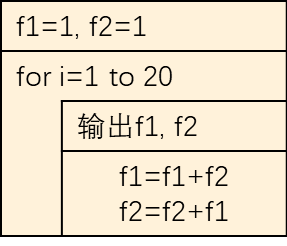
\includegraphics[scale=0.6]{Fn2}\\
	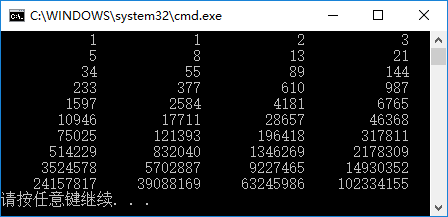
\includegraphics[scale=0.6]{Fno2}
\end{columns}
\end{frame}

\begin{frame}[shrink,fragile]
\small
$[$例5.9$]$输入一个大于3的整数n,判定它是否为素数(prime,又称质数)。
\centering
\begin{columns}
	\column{0.65\textwidth}
\begin{lstlisting}
#include <stdio.h>
int main()
{
  int n,i;
  printf("please enter a integer number,n=?");
  scanf("%d",&n);
  for (i=2;i<n;i++)
    if(n%i==0) break;
  if(i<n) // for提前结束
    printf("%d is not a prime number.\n",n);
  else // for正常结束
    printf("%d is a prime number.\n",n);
  return 0;
}
\end{lstlisting}
	\column{0.3\textwidth}
	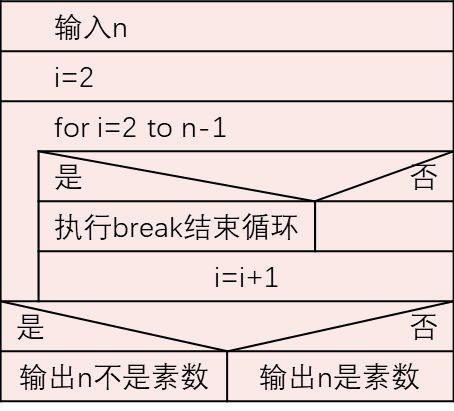
\includegraphics[scale=0.5]{prime}
\end{columns}
\textcolor{blue}{只要在循环结束后检查循环变量i的值,就能判定循环是提前结束还是正常结束的。从而判定n是否为素数。这种判断循环结束的方法以后会常用到。}
\end{frame}

\begin{frame}[shrink,fragile]
\small
\textbf{\textcolor{blue}{优化: }} $n$不必被$2\sim (n-1)$内的各整数去除,只须将$n$被$2\sim\sqrt{n}$之间的整数除即可。因为n的每一对因子, 必然有一个小于n, 另一个大于n。
%\centering
\begin{lstlisting}
#include <stdio.h>
#include <math.h>
int main()
{
   int n,i,k;
   printf("please enter a integer number,n=?");
   scanf("%d",&n);
   k=sqrt(n); // 自动转换为整数(不会四舍五入), 相当于k=(int)sqrt(n);
   for (i=2;i<=k;i++)
     if(n%i==0) break;
   if(i<=k) 
      printf("%d is not a prime number.\n",n);
   else 
      printf("%d is a prime number.\n",n);
   return 0;
}
\end{lstlisting}
\end{frame}

\begin{frame}[shrink,fragile]
\small
\textbf{\textcolor{blue}{使用标志变量, 判断循环结束条件。}}
%\centering
\begin{lstlisting}
int n,i,k,flag=1; // flag: 标志变量
k=sqrt(n); // 自动转换为整数(不会四舍五入), 相当于k=(int)sqrt(n);
for (i=2;i<=k;i++)
   if(n%i==0) { flag=0; break; }
if(!flag) // for提前结束
   printf("%d is not a prime number.\n",n);
else // for正常结束
   printf("%d is a prime number.\n",n);
\end{lstlisting}
\pause
\rule{\textwidth}{1pt} %水平线
\begin{lstlisting}
int n,i,k,flag=1; // flag: 标志变量
k=sqrt(n); // 自动转换为整数(不会四舍五入), 相当于k=(int)sqrt(n);
for (i=2;i<=k && flag;i++) // 比较与上面for的不同
   if(n%i==0) { flag=0; }
if(!flag) 
   printf("%d is not a prime number.\n",n);
else 
   printf("%d is a prime number.\n",n);
\end{lstlisting}
\end{frame}

\begin{frame}[shrink,fragile]
\small
$[$例5.10$]$求$100\sim 200$间的全部素数。
\pause
\begin{lstlisting}
#include <stdio.h>
#include <math.h>
int main()
{
  int n,i,k;
  for (n=101;n<=200;n+=2) //n从101变化到200, 对每个奇数n进行判定
  {
     k=sqrt(n); // 自动转换为整数(不会四舍五入), 相当于k=(int)sqrt(n);
     for(i=2;i<=k;i++)
        if(n%i==0) break;
     if(i>k) 
        printf("%d ",n);
  }
  printf("\n");
  return 0;
}
\end{lstlisting}
\end{frame}

\begin{frame}[shrink,fragile]
$[$例5.11$]$译密码。为使电文保密,往往按一定规律将其转换成密码,收报人再按约定的规律将其译回原文。例如,可以按以下规律将电文变成密码:将字母A变成字母E,a变成e,即变成其后的第4个字母,W变成A,X变成B,Y变成C,Z变成D。
\begin{center}
\begin{tikzpicture}[>=latex, shorten >=1pt,node distance=1cm, on grid, auto,semithick,initial text=, every state/.style={draw=none,minimum size=0.5cm,outer sep=0pt,inner sep=1pt},every label/.style={outer sep=0pt,inner sep=3pt,},every fit/.style={rectangle,rounded corners=3mm,inner xsep=5mm,inner ysep=3mm,outer sep=2pt},font=\small]
\node[state,label={below:0}] (a) {A};
\node[state,label={below:1}] (b) [right= of a] {B};
\node[state,label={below:2}] (c) [right= of b] {C};
\node[state,label={below:3}] (d) [right= of c] {D};
\node[state,label={below:4}] (e) [right= of d] {E};
\node[state,label={below:$\cdots$}] (dot) [right=2cm of e] {$\cdots$};
\node[state,label={below:22}] (w) [right= of dot] {W};
\node[state,label={below:23}] (x) [right= of w] {X};
\node[state,label={below:24}] (y) [right= of x] {Y};
\node[state,label={below:25}] (z) [right= of y] {Z};
\node[] at($(a)+(-0.7,-0.4)$) {Index};
\path[->]
(a) edge[bend right=45] (e)
(w) edge[bend right,dashed,blue] (a)
(x) edge[bend left=45,dashed,red] (b)
;
\end{tikzpicture}
\end{center}
\end{frame}

\begin{frame}[shrink,fragile,plain]
\begin{tikzpicture}[>=latex, shorten >=1pt,node distance=0.7cm, on grid, auto,semithick,initial text=, every state/.style={draw=none,minimum size=0.5cm,outer sep=0pt,inner sep=1pt},every label/.style={outer sep=0pt,inner sep=3pt,},every fit/.style={rectangle,rounded corners=3mm,inner xsep=5mm,inner ysep=3mm,outer sep=2pt},font=\small]
\node[state,label={below:0}] (a) {A};
\node[state,label={below:1}] (b) [right= of a] {B};
\node[state,label={below:2}] (c) [right= of b] {C};
\node[state,label={below:3}] (d) [right= of c] {D};
\node[state,label={below:4}] (e) [right= of d] {E};
\node[state,label={below:$\cdots$}] (dot) [right=2cm of e] {$\cdots$};
\node[state,label={below:22}] (w) [right= of dot] {W};
\node[state,label={below:23}] (x) [right= of w] {X};
\node[state,label={below:24}] (y) [right= of x] {Y};
\node[state,label={below:25}] (z) [right= of y] {Z};
\node[] at($(a)+(-0.7,-0.4)$) {Index};
\path[->]
(a) edge[bend right=45] (e)
(w) edge[bend right,dashed,blue] (a)
(x) edge[bend left=45,dashed,red] (b)
;
\node[anchor=north west,text width=0.9\textwidth,draw] at($(a)+(-0.5,-1.4)$) {
	\vspace{-0.4cm}
	\begin{lstlisting}
	char c;
	c=getchar(); //输入一个字符给字符变量c
	while(c!='\n') //检查c的值是否为换行符'\n'  
	{
		if((c>='a' && c<='z') || (c>='A' && c<='Z')) //c如果是字母
		{
			if((c>='W' && c<='Z') || (c>='w' && c<='z')) c = c-22; //如果是26个字母中最后4个字母之一就使c-22
			else  c =c + 4;   //如果是前面22个字母之一,就使c + 4
		}
		printf("%c",c); //输出已改变的字符
		c=getchar();    //再输入下一个字符给字符变量c
	}
	printf("\n");
	\end{lstlisting}
};
\end{tikzpicture}
\end{frame}

\note{a,b,c,d,e,$\dots$,v(第22个字符),w(c-22),x(c-22),y(c-22),z(c-22)}

\begin{frame}[shrink,fragile]{在循环条件中接收输入的字符是一种常见技巧}
\begin{lstlisting}
char c;
while((c=getchar())!='\n') //检查c的值是否为换行符'\n'  
{
   if((c>='a' && c<='z') || (c>='A' && c<='Z')) //c如果是字母
   {
      if((c>='W' && c<='Z') || (c>='w' && c<='z')) c = c-22; //如果是26个字母中最后4个字母之一就使c-22
      else  c =c + 4;   //如果是前面22个字母之一,就使c + 4
   }
   printf("%c",c); //输出已改变的字符
}
printf("\n");
\end{lstlisting}
\end{frame}
 % ch5, 循环结构程序设计
%%%%%%%%%%%%%%%%%%%%%%%%%%% lecture-7
\begin{frame}[shrink]
  \frametitle{lecture-10 主要内容}
  \framesubtitle{利用数组处理批量数据}
  \tableofcontents[hideallsubsections]
\end{frame}

\begin{frame}[shrink,fragile]{为什么需要数组}
\begin{itemize}
	\item 要向计算机输入全班50个学生的成绩一门课的成绩; 
	\item 用50个float型简单变量表示学生的成绩
	\begin{itemize}
		\item[-] \textbf{烦琐},如果有1000名学生怎么办呢?
		\item[-] 没有反映出这些\textbf{数据间的内在联系},实际上这些数据是同一个班级、同一门课程的成绩,它们具有相同的属性。
	\end{itemize}
\end{itemize}
\begin{lstlisting}
float s0,s1,s2,...,s49; // 50名学生一门课的成绩
\end{lstlisting}
\pause
\begin{lstlisting}
float s[50]; // 50名学生一门课的成绩
int i; // 表示数组下标
for(i=0;i<50;i++) scanf("%f",&s[i]);
\end{lstlisting}
\begin{block}{数组}
	\begin{enumerate}
		\item 数组是一组有序数据的集合。数组中各数据的排列是有一定规律的,下标代表数据在数组中的序号。
		\item 用数组名和下标即可唯一地确定数组中的元素。
		\item 数组中的每一个元素都属于同一个数据类型。
	\end{enumerate}
\end{block}
\end{frame}

\section{定义数组: int a[10];}

\begin{frame}[shrink,fragile]{定义数组: int a[10];}
定义一维数组: \\
\textcolor{blue}{元素类型\quad 数组名[常量表达式(表示元素个数---数组的长度)]}
\begin{lstlisting}
#define NUM 100
float s[50]; // 50名学生一门课的成绩
int a[10]; // 10个元素的整型数组
double b[NUM]; // 常量NUM个元素的double数组
char c[50]; // 50个元素的char型数组
\end{lstlisting}
\begin{block}{Notes}
	数组元素的下标从0开始,int a[10]; 10个整型元素,则最大下标值为9,不存在数组元素a[10]
\end{block}
\begin{tabular}{|c|c|c|c|c|c|c|c|c|c|}
	\hline 
	a[0] & a[1] & a[2] & a[3] & a[4] & a[5] & a[6] & a[7] & a[8] & a[9] \\ 
	\hline 
\end{tabular} 
\end{frame}

\section{引用数组: int i=0; a[i]}

\begin{frame}[shrink,fragile]{引用数组: int i=0; a[i]}
\begin{lstlisting}
int a[10]; // 10个元素的整型数组
int i;
a[0]=10; // 给a数组的第一个元素赋值
a[9]=10; // 给a数组的最后一个元素赋值
printf("%d,%d",a[0],a[9]);
for(i=0;i<10;i++) a[i] = i+1; // 给数组的第i个元素赋值
for(i=0;i<10;i++) printf("%d\t",a[i]); // 输出数组a的10个元素
for(i=0;i<10;i++) scanf("%d",&a[i]); // 输入10个整数, 存入数组a中。注意'&'
\end{lstlisting}
\begin{block}{Notes}
	数组元素的下标从0开始,int a[10]; 10个整型元素,则最大下标值为9,不存在数组元素a[10]
\end{block}
\end{frame}

\begin{frame}[shrink,fragile]
$[$例6.1$]$对10个字符型数组元素依次赋值为'a','b',$\cdots$。要求按逆序输出。
\pause
\begin{lstlisting}
#include <stdio.h>
#define N 10
int main()
{
  char c[N];
  int i;
  for(i=0;i<N;i++) c[i]='a'+i; 
  for(i=N-1;i>=0;i--) printf("%c ", c[i]);
  printf("\n");
  return 0;
}
\end{lstlisting}
\end{frame}

\section{初始化数组: int a[5]=\{1,2,3,4,5\};}

\begin{frame}[shrink,fragile]{初始化数组: int a[5]=\{1,2,3,4,5\};}
为了使程序简洁,常在定义数组的同时给各数组元素赋值,这称为数组的初始化。
\begin{lstlisting}
int a[10]={1,2,3,4,5,6,7,8,9,10}; // 在定义数组时对全部数组元素赋予初值。
char c[10]={'a','b'}; // 可以只给数组中的一部分元素赋值。其他元素的值不确定
double d[]={10.0,10.2,10.3}; // 等效于 double d[3]={10.0,10.2,10.3}
d[2] = 20.2; // 修改第3个元素
\end{lstlisting}
\end{frame}

\begin{frame}[shrink,fragile]
$[$例6.2$]$用数组来处理求Fibonacci数列问题。
\begin{lstlisting}
#include <stdio.h>
#define N 20
int main()
{
  int i;
  int f[N]={1,1};  //对最前面两个元素f[0]和f[1]赋初值1
  for(i=2;i<N;i++)
     f[i]=f[i-2]+f[i-1]; //先后求出f[2]~f[19]的值
  for(i=0;i<N;i++)
  {
     if(i%5==0) printf("\n"); //控制每输出5个数后换行
     printf("%12d",f[i]); //输出一个数
  }
  printf("\n");
  return 0;
}
\end{lstlisting}
\end{frame}

\section{冒泡排序}

\begin{frame}[shrink,fragile]{冒泡排序(第1趟比较)}
int a[4]=\{9,8,5,0\}; // N=4个元素, 要求从小到大顺序排列
\begin{columns}[T]
	\column{0.3\textwidth}
	\begin{tabular}{|c|}
		\hline 
		9 \\ 
		\hline 
		8 \\ 
		\hline 
		5 \\ 
		\hline
		0 \\
	    \hline 
	\end{tabular}\\ 
    第1趟原始数据
	\column{0.2\textwidth}
	\pause
	\begin{tabular}{|c|}
		\hline 
		\colorbox{green}{8} \\ 
		\hline 
		\colorbox{green}{9} \\ 
		\hline 
		5 \\ 
		\hline
		0 \\
		\hline  
	\end{tabular}\\ 
    第1趟第1次相邻两数比较
    \column{0.2\textwidth}
    \pause
    \begin{tabular}{|c|}
    	\hline 
    	\colorbox{green}{8} \\ 
    	\hline 
    	\colorbox{green}{5} \\ 
    	\hline 
    	\colorbox{green}{9} \\ 
    	\hline 
    	0 \\
    	\hline 
    \end{tabular}\\ 
    第1趟第2次相邻两数比较
    \column{0.2\textwidth}
    \pause
    \begin{tabular}{|c|}
    	\hline 
    	\colorbox{green}{8} \\ 
    	\hline 
    	\colorbox{green}{5} \\ 
    	\hline 
    	\colorbox{green}{0} \\ 
    	\hline 
    	\colorbox{yellow}{9} \\
    	\hline 
    \end{tabular}\\ 
    第1趟第3次相邻两数比较(第1个大数沉底)
\end{columns}
~\\
\textcolor{blue}{第j=1趟比较,N-j=3次相邻两数比较}
\end{frame}

\begin{frame}[shrink,fragile]{冒泡排序(第2趟比较)}
int a[4]=\{9,8,5,0\}; // N=4个元素, 要求从小到大顺序排列
\begin{columns}[T]
	\column{0.3\textwidth}
	\begin{tabular}{|c|}
		\hline 
		8 \\ 
		\hline 
		5 \\ 
		\hline 
		0 \\ 
		\hline
		\colorbox{yellow}{9} \\
		\hline 
	\end{tabular}\\ 
	第2趟原始数据
	\column{0.2\textwidth}
	\pause
	\begin{tabular}{|c|}
		\hline 
		\colorbox{green}{5} \\ 
		\hline 
		\colorbox{green}{8} \\ 
		\hline 
		0 \\ 
		\hline
		\colorbox{yellow}{9} \\
		\hline  
	\end{tabular}\\ 
	第2趟第1次相邻两数比较
	\column{0.2\textwidth}
	\pause
	\begin{tabular}{|c|}
		\hline 
		\colorbox{green}{5} \\ 
		\hline 
		\colorbox{green}{0} \\ 
		\hline 
		\colorbox{yellow}{8} \\ 
		\hline 
		\colorbox{yellow}{9} \\
		\hline 
	\end{tabular}\\ 
	第2趟第2次相邻两数比较(第2大沉底)
\end{columns}
~\\
\textcolor{blue}{第j=2趟比较,N-j=2次相邻两数比较}
\end{frame}

\begin{frame}[shrink,fragile]{冒泡排序(第3趟比较)}
int a[4]=\{9,8,5,0\}; // N=4个元素, 要求从小到大顺序排列
\begin{columns}[T]
	\column{0.3\textwidth}
	\begin{tabular}{|c|}
		\hline 
		5 \\ 
		\hline 
		0 \\ 
		\hline 
		\colorbox{yellow}{8} \\ 
		\hline
		\colorbox{yellow}{9} \\
		\hline 
	\end{tabular}\\ 
	第3趟原始数据
	\column{0.2\textwidth}
	\pause
	\begin{tabular}{|c|}
		\hline 
		0 \\ 
		\hline 
		\colorbox{yellow}{5} \\ 
		\hline 
		\colorbox{yellow}{8} \\ 
		\hline
		\colorbox{yellow}{9} \\
		\hline  
	\end{tabular}\\ 
	第3趟第1次相邻两数比较(第3大沉底)
\end{columns}
~\\
\textcolor{blue}{第j=3趟比较,N-j=1次相邻两数比较}
\end{frame}

\begin{frame}[shrink,fragile]{冒泡排序(总结)}
\begin{itemize}
	\setlength{\itemsep}{.5cm}
	\item \#define N 10 // 数组长度
	\item $(N-1)$趟外层循环, $(j=1,2,\cdots,N-1)$, 表示第$j$趟比较。
	\item $(N-j)$次内层循环, $(i=0,1,\cdots, N-1-j)$相邻元素两两比较, 必要时交换。
	\item 注意检查数组边界条件, 不要越界。分别进行N=1, 2, 3, 4个数排序演练。
\end{itemize}
\end{frame}

\begin{frame}[shrink,fragile]{冒泡排序(核心程序)}
\begin{lstlisting}
#define N 10 // 数组长度
int a[N]={9,8,7,6,5,4,3,2,1,0},i,j,t;
for(j=1;j<=N-1;j++) //进行N-1次循环,实现N-1趟比较
{
  for(i=0;i<=N-1-j;i++) //在每一趟中进行N-j次比较相邻元素两两比较
  {
    if(a[i]>a[i+1]) //相邻两个数比较, 注意检查数组不要越界 
       { t=a[i]; a[i]=a[i+1]; a[i+1]=t; } // 交换
  }
}
printf("\n the sorted numbers :\n");
for(i=0;i<N;i++)
   printf("%d ",a[i]);
\end{lstlisting}
\end{frame}

\begin{frame}[shrink,fragile]{冒泡排序(优化)}
\textbf{\textcolor{blue}{优化:第$j$趟排序中, 没有进行相邻元素的交换,表示数据已经排序好, 没有必要进行此后的$(N-j)$趟排序。}}
\begin{lstlisting}
#define N 10 // 数组长度
int a[N]={7,8,7,6,5,6,7,8,9,10},i,j,t,flag;
for(j=1;j<=N-1;j++) //进行N-1次循环,实现N-1趟比较
{
   flag = 0; // 每趟排序,初始化flag,表示未进行交换
   for(i=0;i<=N-1-j;i++) //在每一趟中进行N-j次相邻元素两两比较
   {
     if(a[i]>a[i+1]) //相邻两个数比较, 注意检查数组不要越界 
       { t=a[i]; a[i]=a[i+1]; a[i+1]=t; flag=1; } // 交换, 设置标志变量
   }
   if(!flag) break; // 表示第j趟未交换,排序好了!
}
printf("\n the sorted numbers :\n");
for(i=0;i<N;i++) printf("%d ",a[i]);
\end{lstlisting}
\end{frame}

\begin{frame}[shrink,fragile]{冒泡排序(输出每趟排序的结果)}
\textbf{\textcolor{blue}{优化:第$j$趟排序中, 没有进行相邻元素的交换,表示数据已经排序好, 没有必要进行此后的$(n-j)$趟排序。}}
\begin{lstlisting}
#define N 10 // 数组长度
int a[N]={7,8,7,6,5,6,7,8,9,10},i,j,t,flag;
for(j=1;j<=N-1;j++) //进行N-1次循环,实现N-1趟比较
{
   flag = 0; // 每趟排序,初始化flag,表示未进行交换
   for(i=0;i<=N-1-j;i++) //在每一趟中进行N-j次相邻元素两两比较
   {
      if(a[i]>a[i+1]) //相邻两个数比较, 注意检查数组不要越界 
       { t=a[i]; a[i]=a[i+1]; a[i+1]=t; flag=1; } // 交换, 设置标志变量
   }
   printf("\n 第%d趟排序: \n", j);
   for(t=0;t<N;t++) printf("%d ",a[t]); // 临时变量t的复用
   if(!flag) break; // 表示第j趟未交换,排序好了!
}
printf("\n the sorted numbers :\n");
for(i=0;i<N;i++) printf("%d ",a[i]);
\end{lstlisting}
\end{frame} % ch5, 循环结构程序设计举例
%%%%%%%%%%%%%%%%%%%%%%%%%%% lecture-9
\begin{frame}[shrink]
  \frametitle{lecture-9 主要内容}
  \framesubtitle{循环结构程序设计举例(续)}
  \tableofcontents[hideallsubsections]
\end{frame}

\section{循环结构程序设计举例(续)}

\begin{frame}[fragile]
附加题1: 求$s=a+aa+aaa+\cdots+a\cdots a$, 其中$a$是一个$1\sim 9$的数字。例如$a=2, n=4$时, $s=2+22+222+2222$, $a$和$n$由键盘输入。
\pause
\begin{columns}
\column{0.5\textwidth}
\begin{lstlisting}
int i,s,n,term = 0;
for(i=1,s=0; i<=n; i++) // 初始化循环变量用逗号隔开
{
   term = term*10 + a;
   s += term; 
}
\end{lstlisting}
\end{columns}
\end{frame}

\begin{frame}[fragile]
\small
附加题2: 韩信点兵。韩信有一队兵, 他想知道有多少人, 便让士兵排队报数:\\
按从1至5报数, 最末一个士兵报的数为1;\\
按从1至6报数, 最末一个士兵报的数为5;\\
按从1至7报数, 最末一个士兵报的数为4;\\
按从1至11报数,最末一个士兵报的数为10;\\ 
计算韩信至少有多少兵。 
\pause
\begin{columns}
\column{0.8\textwidth}
\begin{lstlisting}
int x=1;
for(;;x++)  // 循环体仅含if()结构,看作一条语句,'{}'可省略
    if(x%5==1 && x%6==5 && x%7==4 && x%11==10)
    { 
       printf("%d\n",x);  
       break;
    }
\end{lstlisting}
\end{columns}
\end{frame}

\begin{frame}[fragile]
附加题3-1: 求水仙花数。如果一个三位数的个位数、十位数和百位数的立方和等于该数自身,则称该数为水仙花数。 \\
编程求出所有的水仙花数。\\
~\\  
\pause
\begin{columns}
\column{0.6\textwidth}
解法一: 采用三重循环
\begin{lstlisting}
int i,j,k; // 百、十、个位
for(i=1;i<=9;i++)    // 百位
  for(j=0;j<=9;j++)  // 十位
    for(k=0;k<=9;k++)  // 个位
      if(i*100+j*10+k == i*i*i+j*j*j+k*k*k)  
        printf("%d\n",i*100+j*10+k);
\end{lstlisting}
\end{columns}
\end{frame}

\begin{frame}[fragile]
附加题3-2: 求水仙花数。如果一个三位数的个位数、十位数和百位数的立方和等于该数自身,则称该数为水仙花数。 \\
编程求出所有的水仙花数。\\
~\\ 
\pause
\begin{columns}
\column{0.6\textwidth}
解法二: 采用一重循环
\begin{lstlisting}
int m,i,j,k; 
for(m=100;m<=999;m++)
{
   i=m/100; j=m/10%10; k=m%10;  
   if(i*100+j*10+k == i*i*i+j*j*j+k*k*k)  
      printf("%d\n",i*100+j*10+k);
}
\end{lstlisting}
\end{columns}
~\\
\pause
\textcolor{blue}{思考: 输出共有多少个水仙数?}
\end{frame}

\begin{frame}[fragile]
附加题3-3: 求整数区间$[a,b]$中水仙花数的个数。
\pause
\begin{columns}
\column{0.8\textwidth}
\begin{lstlisting}
int n=0; //计数 
int a,b; // a,b 区间
int i,t;   // 循环变量,代表a,b区间的每个数
int sum; // i的各位立方和 
scanf("%d%d",&a,&b);
for(i=a;i<=b;i++) // 考察i是否水仙数
{  
  sum = 0; t=i; // 临时变量记住i; 易遗漏每次内层循环前sum要归0
  while(t!=0) // 累加各位立方 
  { sum+=pow(t%10,3); t=t/10; }
  if(sum==i) n++; // i是水仙数 
}
printf("%d\n",n);
\end{lstlisting}
\end{columns}
\end{frame}

\begin{frame}[fragile]
附加题4: 百钱百鸡, 已知公鸡5个钱1只, 母鸡3个钱1只, 小鸡1个钱3只, 用100个钱买了100只鸡。问公鸡、母鸡、小鸡各几只? 
\vspace{0.5cm}
\pause
\begin{columns}
%\column{0.9\textwidth}
\begin{lstlisting}
int x,y,z; // 公鸡、母鸡、小鸡个数
for(x=0;x<=100;x++) 
   for(y=0;y<=100;y++) 
     for(z=0;z<=100;z++) 
       if(5*x+3*y+z/3 == 100 && x+y+z == 100 && z%3 == 0) // 全部条件! 
          printf("%d,%d,%d\n",x,y,z);
\end{lstlisting}
\end{columns}
\vspace{0.5cm}
\pause
\textcolor{blue}{如何考虑无解的情况?}
\end{frame}

\begin{frame}[shrink,fragile]
附加题5-1: 求整数$a,b$的最大公约数,当两个数中有一个为0时,公约数是不为0的那个整数; 当两个整数互质时最大公约数为1。
输入两个整数a和b,求最大公约数。 
\pause
\begin{lstlisting}
#include <stdio.h>
int main()
{
  int a,b,t,i;
  scanf("%d%d",&a,&b); // 机试系统不要想当然给提示语句, 除非题目要求 
  if(a<b) { t=a; a=b; b=t; } // 交换a,b,使a是较大者 
  for(i=b;i>0;i--)
    if(a%i==0 && b%i==0){ t=i; break; } // 求得最大公约数 
  if(i==0)  // 如果循环结束,还未求得公约数,
  {
    if(b==0) t = a;
    else t=1; // a,b互质 
  } 
  printf("%d\n",t);
  return 0;
}
\end{lstlisting}
\end{frame}

\begin{frame}[shrink,fragile]{求整数$a,b$的最大公约数, 欧几里得算法}
\begin{columns}
	\column{0.6\textwidth}
	古希腊数学家欧几里德在其著作<<The Elements>>中最早描述了这种算法。\\
	\textbf{定理:}两个整数的最大公约数等于其中较小的那个数和两数相除余数的最大公约数。
	\column{0.3\textwidth}
	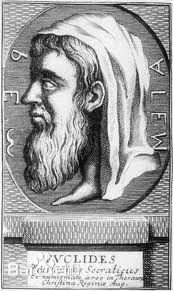
\includegraphics[scale=0.3]{eou}
\end{columns}
~\\
\textbf{伪代码分析}
\begin{lstlisting}
a,b的最大公约数,[则: a=mb+r, m=a/b; r=a%b]
循环, b作被除数,分母是余数r, 
[则: n=b/r; r=nb; a=mb+nb=(m+n)b; 如果一个整数能整除b, 必整除a]
直到r=0, 本轮循环的a(上轮循环的b)就是最大公约数。 
while(1)
{
   r = a%b; // 注意b为0时,不能计算余数,a就是最大公约数
   if(r==0) { gcd=a; break; } // 本轮循环的a(上轮循环的b)就是最大公约数
   a=b; b=r; // 准备下一轮迭代    
}
\end{lstlisting}
\end{frame}

\begin{frame}[shrink,fragile]{求整数$a,b$的最大公约数, 欧几里得算法}
\begin{lstlisting}
int a,b,r,t;
scanf("%d%d",&a,&b); // 机试系统不要想当然给提示语句, 除非题目要求
if(a<b) { t=a; a=b; b=t; } // 交换a,b,使a是较大者
while(1)
{
   if(b==0) { t=a; break; } // 分母为0时, a就是最大公约数
   r = a%b; 
   if(r==0) {t=b; break;} // 本轮循环的a(上轮循环的b)就是最大公约数
   a=b; b=r; // 准备下一轮迭代   
}
printf("%d\n",t);// 输出最大公约数
\end{lstlisting}
\end{frame}

\begin{frame}[shrink,fragile]
附加题6: 给出一个百分制的成绩,要求输出成绩等级'A','B','C','D','E'。90分以上为'A',$80\sim 89$分为'B',$70\sim 79$分为'C',$60\sim 69$分为'D',60分以下为'E'。
\begin{lstlisting}
int grade;
scanf("%d",&grade);
grade /= 10; // 等效于 grade=grade/10;
switch(grade)
{
  case 0: case 1: case 2: case 3: case 4: 
  case 5:  printf("E"); break;
  case 6:  printf("D"); break;
  case 7:  printf("C"); break;
  case 8:  printf("B"); break;
  case 9:
  case 10:  printf("A"); break;
}
\end{lstlisting}
\pause
\textcolor{blue}{思考: 如果输入成绩等级, 输出分数段, 如何修改程序? }
\end{frame}

\begin{frame}{注意事项小结}
\begin{enumerate}
\setlength{\itemsep}{.5cm}
\item while( )\{ \}; do \{ \} while( ); for(;;)\{ \}执行顺序;
\item 循环变量的开始和结束条件;
\item 循环体是复合语句时,必须用\{ \}扩起来;
\item 必要时,用break结束整个循环,用continue结束本次循环;
\item 关键是找出循环规律,必要时设计流程图,指导代码实现。	
\end{enumerate}
\end{frame} % ch5, 循环结构程序设计举例(续)
%%%%%%%%%%%%%%%%%%%%%%%%%%% lecture-7
\begin{frame}[shrink]
  \frametitle{lecture-10 主要内容}
  \framesubtitle{利用数组处理批量数据}
  \tableofcontents[hideallsubsections]
\end{frame}

\begin{frame}[shrink,fragile]{为什么需要数组}
\begin{itemize}
	\item 要向计算机输入全班50个学生的成绩一门课的成绩; 
	\item 用50个float型简单变量表示学生的成绩
	\begin{itemize}
		\item[-] \textbf{烦琐},如果有1000名学生怎么办呢?
		\item[-] 没有反映出这些\textbf{数据间的内在联系},实际上这些数据是同一个班级、同一门课程的成绩,它们具有相同的属性。
	\end{itemize}
\end{itemize}
\begin{lstlisting}
float s0,s1,s2,...,s49; // 50名学生一门课的成绩
\end{lstlisting}
\pause
\begin{lstlisting}
float s[50]; // 50名学生一门课的成绩
int i; // 表示数组下标
for(i=0;i<50;i++) scanf("%f",&s[i]);
\end{lstlisting}
\begin{block}{数组}
	\begin{enumerate}
		\item 数组是一组有序数据的集合。数组中各数据的排列是有一定规律的,下标代表数据在数组中的序号。
		\item 用数组名和下标即可唯一地确定数组中的元素。
		\item 数组中的每一个元素都属于同一个数据类型。
	\end{enumerate}
\end{block}
\end{frame}

\section{定义数组: int a[10];}

\begin{frame}[shrink,fragile]{定义数组: int a[10];}
定义一维数组: \\
\textcolor{blue}{元素类型\quad 数组名[常量表达式(表示元素个数---数组的长度)]}
\begin{lstlisting}
#define NUM 100
float s[50]; // 50名学生一门课的成绩
int a[10]; // 10个元素的整型数组
double b[NUM]; // 常量NUM个元素的double数组
char c[50]; // 50个元素的char型数组
\end{lstlisting}
\begin{block}{Notes}
	数组元素的下标从0开始,int a[10]; 10个整型元素,则最大下标值为9,不存在数组元素a[10]
\end{block}
\begin{tabular}{|c|c|c|c|c|c|c|c|c|c|}
	\hline 
	a[0] & a[1] & a[2] & a[3] & a[4] & a[5] & a[6] & a[7] & a[8] & a[9] \\ 
	\hline 
\end{tabular} 
\end{frame}

\section{引用数组: int i=0; a[i]}

\begin{frame}[shrink,fragile]{引用数组: int i=0; a[i]}
\begin{lstlisting}
int a[10]; // 10个元素的整型数组
int i;
a[0]=10; // 给a数组的第一个元素赋值
a[9]=10; // 给a数组的最后一个元素赋值
printf("%d,%d",a[0],a[9]);
for(i=0;i<10;i++) a[i] = i+1; // 给数组的第i个元素赋值
for(i=0;i<10;i++) printf("%d\t",a[i]); // 输出数组a的10个元素
for(i=0;i<10;i++) scanf("%d",&a[i]); // 输入10个整数, 存入数组a中。注意'&'
\end{lstlisting}
\begin{block}{Notes}
	数组元素的下标从0开始,int a[10]; 10个整型元素,则最大下标值为9,不存在数组元素a[10]
\end{block}
\end{frame}

\begin{frame}[shrink,fragile]
$[$例6.1$]$对10个字符型数组元素依次赋值为'a','b',$\cdots$。要求按逆序输出。
\pause
\begin{lstlisting}
#include <stdio.h>
#define N 10
int main()
{
  char c[N];
  int i;
  for(i=0;i<N;i++) c[i]='a'+i; 
  for(i=N-1;i>=0;i--) printf("%c ", c[i]);
  printf("\n");
  return 0;
}
\end{lstlisting}
\end{frame}

\section{初始化数组: int a[5]=\{1,2,3,4,5\};}

\begin{frame}[shrink,fragile]{初始化数组: int a[5]=\{1,2,3,4,5\};}
为了使程序简洁,常在定义数组的同时给各数组元素赋值,这称为数组的初始化。
\begin{lstlisting}
int a[10]={1,2,3,4,5,6,7,8,9,10}; // 在定义数组时对全部数组元素赋予初值。
char c[10]={'a','b'}; // 可以只给数组中的一部分元素赋值。其他元素的值不确定
double d[]={10.0,10.2,10.3}; // 等效于 double d[3]={10.0,10.2,10.3}
d[2] = 20.2; // 修改第3个元素
\end{lstlisting}
\end{frame}

\begin{frame}[shrink,fragile]
$[$例6.2$]$用数组来处理求Fibonacci数列问题。
\begin{lstlisting}
#include <stdio.h>
#define N 20
int main()
{
  int i;
  int f[N]={1,1};  //对最前面两个元素f[0]和f[1]赋初值1
  for(i=2;i<N;i++)
     f[i]=f[i-2]+f[i-1]; //先后求出f[2]~f[19]的值
  for(i=0;i<N;i++)
  {
     if(i%5==0) printf("\n"); //控制每输出5个数后换行
     printf("%12d",f[i]); //输出一个数
  }
  printf("\n");
  return 0;
}
\end{lstlisting}
\end{frame}

\section{冒泡排序}

\begin{frame}[shrink,fragile]{冒泡排序(第1趟比较)}
int a[4]=\{9,8,5,0\}; // N=4个元素, 要求从小到大顺序排列
\begin{columns}[T]
	\column{0.3\textwidth}
	\begin{tabular}{|c|}
		\hline 
		9 \\ 
		\hline 
		8 \\ 
		\hline 
		5 \\ 
		\hline
		0 \\
	    \hline 
	\end{tabular}\\ 
    第1趟原始数据
	\column{0.2\textwidth}
	\pause
	\begin{tabular}{|c|}
		\hline 
		\colorbox{green}{8} \\ 
		\hline 
		\colorbox{green}{9} \\ 
		\hline 
		5 \\ 
		\hline
		0 \\
		\hline  
	\end{tabular}\\ 
    第1趟第1次相邻两数比较
    \column{0.2\textwidth}
    \pause
    \begin{tabular}{|c|}
    	\hline 
    	\colorbox{green}{8} \\ 
    	\hline 
    	\colorbox{green}{5} \\ 
    	\hline 
    	\colorbox{green}{9} \\ 
    	\hline 
    	0 \\
    	\hline 
    \end{tabular}\\ 
    第1趟第2次相邻两数比较
    \column{0.2\textwidth}
    \pause
    \begin{tabular}{|c|}
    	\hline 
    	\colorbox{green}{8} \\ 
    	\hline 
    	\colorbox{green}{5} \\ 
    	\hline 
    	\colorbox{green}{0} \\ 
    	\hline 
    	\colorbox{yellow}{9} \\
    	\hline 
    \end{tabular}\\ 
    第1趟第3次相邻两数比较(第1个大数沉底)
\end{columns}
~\\
\textcolor{blue}{第j=1趟比较,N-j=3次相邻两数比较}
\end{frame}

\begin{frame}[shrink,fragile]{冒泡排序(第2趟比较)}
int a[4]=\{9,8,5,0\}; // N=4个元素, 要求从小到大顺序排列
\begin{columns}[T]
	\column{0.3\textwidth}
	\begin{tabular}{|c|}
		\hline 
		8 \\ 
		\hline 
		5 \\ 
		\hline 
		0 \\ 
		\hline
		\colorbox{yellow}{9} \\
		\hline 
	\end{tabular}\\ 
	第2趟原始数据
	\column{0.2\textwidth}
	\pause
	\begin{tabular}{|c|}
		\hline 
		\colorbox{green}{5} \\ 
		\hline 
		\colorbox{green}{8} \\ 
		\hline 
		0 \\ 
		\hline
		\colorbox{yellow}{9} \\
		\hline  
	\end{tabular}\\ 
	第2趟第1次相邻两数比较
	\column{0.2\textwidth}
	\pause
	\begin{tabular}{|c|}
		\hline 
		\colorbox{green}{5} \\ 
		\hline 
		\colorbox{green}{0} \\ 
		\hline 
		\colorbox{yellow}{8} \\ 
		\hline 
		\colorbox{yellow}{9} \\
		\hline 
	\end{tabular}\\ 
	第2趟第2次相邻两数比较(第2大沉底)
\end{columns}
~\\
\textcolor{blue}{第j=2趟比较,N-j=2次相邻两数比较}
\end{frame}

\begin{frame}[shrink,fragile]{冒泡排序(第3趟比较)}
int a[4]=\{9,8,5,0\}; // N=4个元素, 要求从小到大顺序排列
\begin{columns}[T]
	\column{0.3\textwidth}
	\begin{tabular}{|c|}
		\hline 
		5 \\ 
		\hline 
		0 \\ 
		\hline 
		\colorbox{yellow}{8} \\ 
		\hline
		\colorbox{yellow}{9} \\
		\hline 
	\end{tabular}\\ 
	第3趟原始数据
	\column{0.2\textwidth}
	\pause
	\begin{tabular}{|c|}
		\hline 
		0 \\ 
		\hline 
		\colorbox{yellow}{5} \\ 
		\hline 
		\colorbox{yellow}{8} \\ 
		\hline
		\colorbox{yellow}{9} \\
		\hline  
	\end{tabular}\\ 
	第3趟第1次相邻两数比较(第3大沉底)
\end{columns}
~\\
\textcolor{blue}{第j=3趟比较,N-j=1次相邻两数比较}
\end{frame}

\begin{frame}[shrink,fragile]{冒泡排序(总结)}
\begin{itemize}
	\setlength{\itemsep}{.5cm}
	\item \#define N 10 // 数组长度
	\item $(N-1)$趟外层循环, $(j=1,2,\cdots,N-1)$, 表示第$j$趟比较。
	\item $(N-j)$次内层循环, $(i=0,1,\cdots, N-1-j)$相邻元素两两比较, 必要时交换。
	\item 注意检查数组边界条件, 不要越界。分别进行N=1, 2, 3, 4个数排序演练。
\end{itemize}
\end{frame}

\begin{frame}[shrink,fragile]{冒泡排序(核心程序)}
\begin{lstlisting}
#define N 10 // 数组长度
int a[N]={9,8,7,6,5,4,3,2,1,0},i,j,t;
for(j=1;j<=N-1;j++) //进行N-1次循环,实现N-1趟比较
{
  for(i=0;i<=N-1-j;i++) //在每一趟中进行N-j次比较相邻元素两两比较
  {
    if(a[i]>a[i+1]) //相邻两个数比较, 注意检查数组不要越界 
       { t=a[i]; a[i]=a[i+1]; a[i+1]=t; } // 交换
  }
}
printf("\n the sorted numbers :\n");
for(i=0;i<N;i++)
   printf("%d ",a[i]);
\end{lstlisting}
\end{frame}

\begin{frame}[shrink,fragile]{冒泡排序(优化)}
\textbf{\textcolor{blue}{优化:第$j$趟排序中, 没有进行相邻元素的交换,表示数据已经排序好, 没有必要进行此后的$(N-j)$趟排序。}}
\begin{lstlisting}
#define N 10 // 数组长度
int a[N]={7,8,7,6,5,6,7,8,9,10},i,j,t,flag;
for(j=1;j<=N-1;j++) //进行N-1次循环,实现N-1趟比较
{
   flag = 0; // 每趟排序,初始化flag,表示未进行交换
   for(i=0;i<=N-1-j;i++) //在每一趟中进行N-j次相邻元素两两比较
   {
     if(a[i]>a[i+1]) //相邻两个数比较, 注意检查数组不要越界 
       { t=a[i]; a[i]=a[i+1]; a[i+1]=t; flag=1; } // 交换, 设置标志变量
   }
   if(!flag) break; // 表示第j趟未交换,排序好了!
}
printf("\n the sorted numbers :\n");
for(i=0;i<N;i++) printf("%d ",a[i]);
\end{lstlisting}
\end{frame}

\begin{frame}[shrink,fragile]{冒泡排序(输出每趟排序的结果)}
\textbf{\textcolor{blue}{优化:第$j$趟排序中, 没有进行相邻元素的交换,表示数据已经排序好, 没有必要进行此后的$(n-j)$趟排序。}}
\begin{lstlisting}
#define N 10 // 数组长度
int a[N]={7,8,7,6,5,6,7,8,9,10},i,j,t,flag;
for(j=1;j<=N-1;j++) //进行N-1次循环,实现N-1趟比较
{
   flag = 0; // 每趟排序,初始化flag,表示未进行交换
   for(i=0;i<=N-1-j;i++) //在每一趟中进行N-j次相邻元素两两比较
   {
      if(a[i]>a[i+1]) //相邻两个数比较, 注意检查数组不要越界 
       { t=a[i]; a[i]=a[i+1]; a[i+1]=t; flag=1; } // 交换, 设置标志变量
   }
   printf("\n 第%d趟排序: \n", j);
   for(t=0;t<N;t++) printf("%d ",a[t]); // 临时变量t的复用
   if(!flag) break; // 表示第j趟未交换,排序好了!
}
printf("\n the sorted numbers :\n");
for(i=0;i<N;i++) printf("%d ",a[i]);
\end{lstlisting}
\end{frame} % ch6, 一维数组,冒泡排序
%%%%%%%%%%%%%%%%%%%%%%%%%%% lecture-11
%\begin{frame}[shrink]
%  \frametitle{lecture-11 主要内容}
%  \framesubtitle{字符串处理库函数及程序举例}
%  %\tableofcontents[hideallsubsections]
%  \tableofcontents
%\end{frame}

\section{字符串处理函数\#include<string.h>}

\begin{frame}[shrink,fragile]{字符串处理函数\#include<string.h>}
\vspace{-0.2cm}
\begin{itemize}
	\item 使用字符串处理库函数, 必须包含头文件\#include<string.h>
	\item 要求字符串必须以`$\backslash$0'结尾
\end{itemize}
\vspace{-0.2cm}
\begin{lstlisting}
#include<stdio.h>
#include<string.h>
int main()
{
   char s1[81]="ab"; // 自动追加s1[2]='\0'
   char s2[81]="cdef"; // 自动追加s2[4]='\0'
   
   // 连接两个字符串, 结果被放入s1中, s1数组要足够大,能够容纳两个字符串连接后的长度+1, 多一个字符长度是留给'\0'使用
   strcat(s1,s2); 
   
   puts(s1); // abcdef, 最后一个字符是'\0'
   puts(s2); // cdef, 保持不变, , 最后一个字符是'\0'
   return 0;
}
\end{lstlisting}
\end{frame}

\subsection{连接和复制字符串strcat(s1,s2); strcpy(s1,s2); strncpy(s1,s2,n)}

\begin{frame}[shrink,fragile]{\small{连接和复制字符串strcat(s1,s2); strcpy(s1,s2); strncpy(s1,s2,n)}}
\vspace{-0.3cm}
\begin{lstlisting}
   char s1[81]="ab"; // 自动追加s1[2]='\0'
   char s2[81]="cdef"; // 自动追加s2[4]='\0'
   // 连接两个字符串, 结果被放入s1中, s1数组要足够大,能够容纳两个字符串连接后的长度+1, 多一个字符长度是留给'\0'使用
   strcat(s1,s2); 
   puts(s1); // abcdef, 最后一个字符是'\0'
   puts(s2); // cdef, 保持不变, , 最后一个字符是'\0'
   // 把s2复制给s1, 因此s1数组也要足够大
   strcpy(s1,s2);  // s1=s2; 是错误的, 因为数组名表示地址常量
   puts(s1); // cdef, 最后一个字符是'\0'
   puts(s2); // cdef, 保持不变, , 最后一个字符是'\0'
   strncpy(s1,"1234",2); // 复制s2的前n个字符给s1,覆盖s1相应位置的字符, n要小于s1的数组长度
   puts(s1); // 12ef
\end{lstlisting}
\end{frame}

\subsection{字符串比较strcmp(s1,s2); strncmp(s1,s2,n)}

\begin{frame}[shrink,fragile]{字符串比较strcmp(s1,s2); strncmp(s1,s2,n)}
\begin{lstlisting}
   char s1[81]="ab"; // 自动追加s1[2]='\0'
   char s2[81]="cdef"; // 自动追加s2[4]='\0'
   // 从左到右逐字符比较串s1和s2,大于返回1, 小于返回-1, 同时到达'\0'返回0表示相等
   printf("%d",strcmp(s1,s2)); // -1
   if(strcmp(s1,s2)==-1) printf("s1 < s2\n");
   printf("%d\n",strcmp("abad","ab1d")); // 1
   printf("%d\n",strcmp("1234","1234")); // 0
   printf("%d\n",strcmp("12","1234")); // -1
   printf("%d\n",strcmp("1234","12")); // 1  
   // 仅比较前n个字符
   printf("%d\n",strncmp("1234","12",2)); // 0
\end{lstlisting}
\end{frame}

\subsection{获取字符串的长度strlen(s)}

\begin{frame}[shrink,fragile]{获取字符串的长度strlen(s)}
\begin{lstlisting}
   char s1[81]="ab"; // 自动追加s1[2]='\0'
   char s2[81]="cdef"; // 自动追加s2[4]='\0'
   int i;
   // 获取字符串的长度,不包括字符串结尾字符'\0'
   printf("%d,%d\n",strlen(s1), strlen(s2)); // 2,4
   for(i=0;i<strlen(s1);i++) printf("%c ",s[i]); // a b
   // 相当于下面程序段计算出的字符串长度len
   int len=0;
   for(i=0; s1[i]!='\0'; i++) len++;
   printf("\n字符串s1的长度=%d\n", len);
\end{lstlisting}
\end{frame}

\subsection{大小写转换strlwr(s); strupr(s)}

\begin{frame}[shrink,fragile]{大小写转换strlwr(s); strupr(s)}
\begin{lstlisting}
char s1[81]="abCD12"; // 自动追加s1[2]='\0'
char s2[81]="cD12ef"; // 自动追加s2[4]='\0'
int i;
strlwr(s1); // 大写转小写
puts(s1); // abcd12
 
strupr(s2); // 小写转大写
puts(s2); // CD12EF

// 小写转大写, 等效于下面程序段
for(i=0;s2[i]!='\0';i++)
  if(s2[i]>='a' && s2[i]<='z') s2[i]-=32;  // s2[i]=s2[i]-32
\end{lstlisting}
\end{frame}

\section{程序举例}

\subsection{统计单词数}

\begin{frame}[shrink,fragile]{\small{例6.8 输入一行字符, 统计其中有多少个单词, 单词之间用空格(可能多个)分隔开。}}
\pause
\begin{lstlisting}
// 定义变量
char string[81]; // 用于存放字符串。
int i; // 计数器,用于遍历字符串中的每个字符。
int word=0; // 用于判断是否开始了一个新单词的标志。若word=0表示未出现新单词, 如出现了新单词, 就把word置成1。
int num=0; //用于统计单词数。
\end{lstlisting}
\pause
\begin{multicols}{3}
	构思程序流程$\implies$\\
	\includegraphics<3->[scale=0.45]{ex6-8}
\end{multicols}
\end{frame}

\begin{frame}[shrink,fragile]{\small{解: 例6.8 输入一行字符, 统计其中有多少个单词, 单词之间用空格(可能多个)分隔开。}}
\begin{lstlisting}
char string[81];
int i,num=0,word=0;
char c;
gets(string); //输入一个字符串给字符数组string
for(i=0;(c=string[i])!='\0';i++) //只要字符不是'\0'就循环,条件表达式:第i个字符赋值给c, 并且c$\ne$'\0'
{
   if(c==' ') word=0; //若是空格字符,使word置0
   else if(word==0) //如果不是空格字符且word原值为0
   { 
     word=1; //使word置1
     num++; //num累加1,表示增加一个单词
   }
}
printf("%d words in this line.\n",num); //输出单词数
\end{lstlisting}
\end{frame}

\subsection{求多个字符串中的较大者}

\begin{frame}[shrink,fragile]{\small{例6.9 有3个字符串,要求找出其中``最大"者。}}
\pause
\begin{lstlisting}
char str[3][20]; //定义二维字符数组, 存放3个字符串。【重点学习】
char string[20]; //定义一维字符数组,作为交换字符串时的临时字符数组
int i;
for(i=0;i<3;i++)
   gets(str[i]); //读入3个字符串,分别给str[0],str[1],str[2]

if(strcmp(str[0],str[1])>0) //若str[0]大于str[1]
     strcpy(string,str[0]); //把str[0]的字符串赋给字符数组string
else //若str[0]小于等于str[1]
     strcpy(string,str[1]); //把str[1]的字符串赋给字符数组string 
if(strcmp(str[2],string)>0) //若str[2]大于string
     strcpy(string,str[2]); //把str[2]的字符串赋给字符数组string
printf("\nthe largest string is:\n%s\n",string); //输出string
\end{lstlisting}
\end{frame}


\begin{frame}[shrink,fragile]{\small{另解: 例6.9 有3个字符串,要求找出其中``最大"者。}}
\begin{lstlisting}
#include<stdio.h>
#include<string.h>
int main()                   
{  
   char s[20],max[20];  int i;
   for(i=0;i<3;i++)
   {
      if(i==0)gets(max); // 常用技巧: 初始, 第一个字符串就是最大者。
      else // 随后的字符串与max比较
      {
         gets(s);
         if(strcmp(s,max)>0) strcpy(max,s); // 如果该字符串比max大, 替换之。
      }
   }
   printf("\nthe largest string is:\n%s\n",max);
   return 0;           
}
\end{lstlisting}
\end{frame}  

\subsection{矩阵乘法}

\begin{frame}[shrink,fragile]{例: 矩阵乘法}
\vspace{-0.4cm}
\begin{align*}
&c[M][N],a[M][P],b[P][N];\\ &c[i][j]=\sum_{k=0}^{P-1}a[i][k]b[k][j]=a[i][0]b[0][j]+a[i][1]b[1][j]+\cdots +a[i][P-1]b[P-1][j]
\end{align*}
\begin{scriptsize}
\begin{align*}
&a=\left[\begin{array}[l]{ccc}
a[0][0] & a[0][1] & a[0][2]\\
a[1][0] & a[1][1] & a[1][2]
\end{array}
\right]\quad
b=\left[\begin{array}[l]{ccc}
b[0][0] & b[0][1] \\
b[1][0] & b[1][1] \\
b[2][0] & b[2][1]
\end{array}
\right]\\
&c=\left[\begin{array}[l]{ccc}
a[0][0]b[0][0]+a[0][1]b[1][0]+a[0][2]b[2][0] & a[0][0]b[0][1]+a[0][1]b[1][1]+a[0][2]b[2][1] \\
a[1][0]b[0][0]+a[1][1]b[1][0]+a[1][2]b[2][0] & a[1][0]b[0][1]+a[1][1]b[1][1]+a[1][2]b[2][1]
\end{array}
\right]
\end{align*}
\end{scriptsize}
\\
%\vspace{0.2cm}
%\medskip
\pause
\bigskip
\textbf{\textcolor{blue}{c[i][j]=a的第i行各列(k)和b的第j列各行(k)的乘积累加. $k=0\to(P-1)$}}
\end{frame}

\begin{frame}[shrink,fragile]{解: 矩阵乘法}
\begin{lstlisting}
#define M 100 // 估计的最大值
#define P 50
#define N 100 
int c[M][N],a[M][P]={{1,2,4}},b[P][N]={{2,1,3},{7,9,10},{5,7,1}}; // c={36,47,27}
int m=4,n=2,p=3; // M,N,P实际大小
int i,j,k; //i,j,k分别是m,n,p的循环变量 
for(i=0;i<m;i++) 
{
   for(j=0;j<n;j++)
   {
     c[i][j]=0;
     for(k=0;k<p;k++) 
        c[i][j]+=a[i][k]*b[k][j]; // a的第i行各列(k)和b的第j列各行(k)的乘积累加 
     printf("c[%d][%d]=%d\n",i,j,c[i][j]); // 输出测试
   }
}
\end{lstlisting}
\end{frame}

\begin{frame}[shrink,fragile]
\small{曾经的测试用例}
\begin{lstlisting}
//int c[M][N],a[M][P]={{1,2,4}},b[P][N]={{2,1,3},{7,9,10},{5,7,1}}; // c={36,47,27}
//int m=1,n=3,p=3; // M,N,P实际大小
//int c[M][N],a[M][P]={{2,1},{4,3}},b[P][N]={{1,2},{1,0}}; // c={{3,4},{7,8}}
//int m=2,n=2,p=2; // M,N,P实际大小
//int c[M][N],a[M][P]={{1,0,2},{-1,3,1}},b[P][N]={{3,1},{2,1},{1,0}}; // c={{5,1},{4,2}}
//int m=2,n=2,p=3; // M,N,P实际大小
int c[M][N],a[M][P]={{5,2,4},{3,8,2},{6,0,4},{0,1,6}},b[P][N]={{2,4},{1,3},{3,2}}; // c={{24,34},{20,40},{24,32},{19,15}}
int m=4,n=2,p=3; // M,N,P实际大小
int i,j,k; //i,j,k分别是m,n,p的循环变量  
// 添加输入语句
scanf("%d%d%d\n", &m,&n,&p);
for(i=0;i<m;i++)
  for(k=0;k<p;k++) scanf("%d",&a[i][k]);
for(k=0;k<p;k++)
  for(j=0;j<n;j++) scanf("%d",&b[k][j]);
...
\end{lstlisting}
\end{frame}  

%\begin{frame}[shrink]
%\frametitle{lecture-12 主要内容}
%\framesubtitle{字符串处理库函数及程序举例}
%%\tableofcontents[hideallsubsections]
%\tableofcontents
%\end{frame}               






 % ch6, 二维数组和字符数组
%%%%%%%%%%%%%%%%%%%%%%%%%%% lecture-12
%\begin{frame}[shrink]
%  \frametitle{lecture-12 主要内容}
%  \framesubtitle{用函数实现模块化程序设计}
%  %\tableofcontents[hideallsubsections]
%  \tableofcontents
%\end{frame}

\section{使用函数进行模块化程序设计}

\begin{frame}[shrink,fragile]{为什么使用函数(1)}
\tiny
\vspace{-0.2cm}
\begin{columns}[T]
\column{0.4\textwidth}
\begin{beamerboxesrounded}{函数调用}
\begin{lstlisting}
#include<stdio.h>
#include<math.h>
int main() // 主函数
{
   int a;
   // 库函数调用
   scanf("%d",&a); 
   a=(int)fabs(a); 
   printf("%d\n",a);
   return 0; 
}
\end{lstlisting}
\end{beamerboxesrounded}
\column{0.6\textwidth}
\begin{beamerboxesrounded}{函数定义}
\begin{lstlisting}
int scanf(char format[], args, ...)
{ ...;
  return 整型值;
}
int printf(char format[], args, ...)
{ ...;
  return 整型值;
}
double fabs(double a)
{ // 模拟代码,没有考虑精度
  if(a<0) return -a;
  else return a;
}
\end{lstlisting}
\end{beamerboxesrounded}
\end{columns}
\end{frame}

\begin{frame}[shrink,fragile]{为什么使用函数(2)}
\tiny
\vspace{-0.2cm}
\begin{columns}[T]
\column{0.5\textwidth}
\begin{beamerboxesrounded}{函数调用}
\begin{lstlisting}
#include<stdio.h>
#include<string.h>
int main() // 主函数
{
   int a;
   char s1[81],char s2[81]="1234";
   // 库函数调用 
   strcpy(s1,s2); 
   a=strcmp(s1,s2);
   printf("%d ",a);
   printf("%d\n",strlen(s1));
   return 0; 
}
\end{lstlisting}
\end{beamerboxesrounded}
\column{0.5\textwidth}
\begin{beamerboxesrounded}{函数定义}
\begin{lstlisting}
char[] strcpy(char s1[],char s2[])
{ ...; return s1; 
}
int strcmp(char s1[],char s2[])
{  ...;  return 整型值; // 1,-1,0
}
int strlen(char s[])
{
  int len=0;
  while(s[len]!='\0') len++;
  return len;
}
\end{lstlisting}
\end{beamerboxesrounded}
\end{columns}
\end{frame}

\begin{frame}[shrink,fragile]{利用函数进行功能分解 --- 简化程序设计的有效手段}
\vspace{-0.3cm}
\begin{columns}[T]
\column{0.5\textwidth}
\begin{beamerboxesrounded}{功能分解, 函数调用}
\begin{lstlisting}
#include<stdio.h>
#include<math.h>
int add(int a,int b); // 函数原型声明
void output(double a);
int main() // 主函数
{
  int a=10,b=20,c;
  //传递参数a,b的值, 计算结果赋值给变量c 
  c=add(a,b);  // 函数调用
  output(10.5*c); // 函数调用
  return 0; 
}
\end{lstlisting}
\end{beamerboxesrounded}
\column{0.5\textwidth}
\begin{beamerboxesrounded}{分解功能实现, 函数定义}
\begin{lstlisting}
// 通过参数a,b的值, 进行相关计算, 返回整型数据给调用者
int add(int a,int b)
{  return a+b; // 返回整型值 }
// 通过参数a的值, 进行相关计算, 不需要返回数据
void output(double a)
{  
   printf("%lf\n", sqrt(a)); // 函数中可调用别的函数
}
\end{lstlisting}
\end{beamerboxesrounded}
\end{columns}
%~\\
\end{frame}

\begin{frame}{使用函数进行程序设计的优点}
\begin{enumerate}
	\setlength{\itemsep}{.5cm}
	\item 使用函数可使程序清晰、精炼、简单、灵活。
	\item 函数就是功能。每一个函数用来实现一个特定的功能。函数名应反映其代表的功能。
	\item 在设计较大程序时,往往把它分为若干个程序模块,每一个模块包括一个或多个函数,每个函数实现一个特定的功能。
	\item 一个C程序可由一个主函数和若干个其他函数构成。由主函数调用其他函数,其他函数也可以互相调用。	
\end{enumerate}
\end{frame}

%\subsection{函数三要素: 函数原型声明, 函数定义, 函数调用}

\begin{frame}[shrink,fragile]{函数三要素: 函数原型声明, 函数定义, 函数调用}
\vspace{-0.2cm}
\begin{columns}[T]
\column{0.5\textwidth}
\begin{beamerboxesrounded}{函数原型声明, 函数调用}
\begin{lstlisting}
#include<stdio.h> // 库函数原型声明
// 函数原型声明, 使编译器认识这个函数,如果函数定义在调用之前,可省略声明
int add(int a,int b); 
void output(double a);
int main() // 主函数
{
   int a=10,b=20,c;
   // 函数调用, 执行函数功能
   c=add(a,b); 
   output(10.5*c);
   return 0; 
}
\end{lstlisting}
\end{beamerboxesrounded}
\column{0.5\textwidth}
\begin{beamerboxesrounded}{函数定义, 定义函数功能}
\begin{lstlisting}
// 通过参数a,b的值, 进行相关计算, 返回整型数据给调用者
int add(int a,int b)
{  return a+b; // 返回整型值 }

// 通过参数a的值, 进行相关计算, 不需要返回数据
void output(double a)
{  
   printf("%lf\n", sqrt(a)); // 函数中可调用别的函数
}
\end{lstlisting}
\end{beamerboxesrounded}
\end{columns}
~\\
\end{frame}

%\subsection{函数定义: int\, add(int a,int b)\{\quad\}}

\begin{frame}[shrink,fragile]{函数定义: int\, add(int a,int b)\{\quad\}}
\textbf{函数定义: } 返回类型\, 函数名(参数类型\, 参数, $\cdots$) $\{\cdots ; \}$
\begin{lstlisting}
int add(int a, int b)
{  ...;
   return 整型值; // 必须含return语句, 函数执行结束, 并将返回值返回给调用者
}
double fun(void) // 无参函数, 等效 double fun() 
{  ...;
   return 双精度值; // 必须含return语句, 函数执行结束, 并将返回值返回给调用者
}
void output(double a) // 无返回值函数
{  ...;
   return; // 可选return语句(注意没有表达式), 仅表示函数执行结束
}
\end{lstlisting}
\end{frame}

\begin{frame}[shrink,fragile]{函数调用时数据类型的隐式转换}
\begin{lstlisting}
int a=2,b=3,c;
// pow函数原型: double pow(double x,double y);
// 编译器自动把a,b"隐式"转换为double
// 计算$a^b$的结果是double类型, 赋值语句隐式转换为int, 但是会引起警告信息
c=pow(a,b);
c=(int)pow(a,b); // 将函数的返回值强制转换为int, 不会有警告信息
c=(int)pow((double)a,(double)b); // 例如vs2019等编译器要求显示强制转换
\end{lstlisting}
\end{frame}

\begin{frame}[shrink,fragile]{整数pow函数问题}
\vspace{-0.3cm}
\lstinline|double pow(double x,double y);| 数学库函数真对双精度浮点数设计。用它计算整数$x^y$会有复杂的精度问题, 因此整数运算尽量不要用此函数。 
\begin{lstlisting}
#include<stdio.h>
#include<math.h>   // 数学库函数
int main()
{
	int x=2,y=3;
	// 有些编译器会输出99,124, 因为转换前是99.999, 124.999 
	printf("%d,%d\n",(int)pow(10,x),(int)pow(5,y)); 	
	// 奇怪的是下列调用输出结果与上面有可能会输出不一致的结果 
	printf("%d,%d\n",(int)pow(10,2),(int)pow(5,3)); 
	return 0;
}
\end{lstlisting}
\end{frame}

\begin{frame}[shrink,fragile]{自定义整数pow函数}
\vspace{-0.5cm}
\begin{columns}[T]
\column{0.35\linewidth}
\begin{lstlisting}
#include<stdio.h>
// 自定义整数pow函数
int intpow(int x, int y)
{
	int i,p=1;
	if(x==0) return 0; 
	for(i=0;i<y;i++)p=p*x;
	return p;
} 
\end{lstlisting}
\column{0.65\linewidth}
\begin{lstlisting}[frame=leftline]
int main()
{
	int x=2,y=3;
	
	printf("%d,%d\n",intpow(10,x),intpow(5,y)); 
	// 100,125
	printf("%d,%d\n",intpow(10,2),intpow(5,3)); 
	// 100,125
	printf("%d,%d\n",intpow(0,2),intpow(0,0)); 
	// 0,1 
	
	return 0;
}
\end{lstlisting}
\end{columns}
\end{frame}

\note{递归版
	\begin{lstlisting}
	int intpow(int x,int y)
	{
		if(x==0) return 0; // 0^y=0 
		// 递归 
		if(y==0) return 1; // x^0=1, 结束递归
		else if(y%2) return x*intpow(x,y/2)*intpow(x,y/2);
		return intpow(x,y/2)*intpow(x,y/2);
	}
    \end{lstlisting}
}

\section{实参和形参间的数据传递(值传递和地址传递)}

\begin{frame}[shrink,fragile]{实参和形参间的数据传递(值传递)}
\vspace{-0.3cm}
\begin{columns}[T]
\column{0.55\textwidth}
\begin{lstlisting}
#include<stdio.h> // 库函数原型声明
// 函数原型声明, 使编译器认识这个函数
int max(int x,int y); 
int main() // 主函数
{
   int a=10,b=20,c;
   scanf("%d%d",&a,&b);
   // 把此处的a,b值拷贝给函数形式参数x,y
   c=max(a,b); // 实际参数 
   printf("较大者=%d\n",c);//与下一句等效
   printf("较大者=%d\n",max(a,b));
   return 0; 
}
\end{lstlisting}
\column{0.45\textwidth}
\begin{lstlisting}[frame=leftline]
// 定义函数求形参x,y中的较大者并返回给调用者
int max(int x,int y) // 形式参数
{  
   int z;
   z=x>y ? x : y;
   return z; 
}
\end{lstlisting}
\end{columns}
\textbf{\textcolor{blue}{在调用函数过程中发生的实参与形参间的数据传递称为``虚实结合"。}}
\end{frame}

\begin{frame}[shrink,fragile]{实参和形参间的数据传递(地址传递)}
例: 将数组a中n个整数按相反顺序存放。
\begin{columns}[T]
\column{0.6\textwidth}
\begin{lstlisting}
#include<stdio.h> 
void inv(int x[],int n); // 要求x是地址传递
#define N 100 
int main() 
{
   int i, n, a[N]={1,2,3,4,5,6,7,8,9,10};
   scanf("%d",&n);
   for(i=0; i<n; i++) scanf("%d",&a[i]);
   // 把实参a数组的地址拷贝给形参x, n的值拷贝给形式参数n
   inv(a,n); // 实参a数组的内容被改变
   for(i=0; i<n; i++) printf("%d ",a[i]);
   return 0; 
}
\end{lstlisting}
\column{0.4\textwidth}
\begin{lstlisting}[frame=leftline]
// 倒置数组x的内容, n是x的长度
// 要求x是地址传递
void inv(int x[],int n) 
{  
   int i,temp,m=(n-1)/2;
   //以中间元素为界, 前后元素交换
   for(i=0; i<=m; i++) 
   {
      temp=x[i]; 
      x[i]=x[n-1-i]; 
      x[n-1-i]=temp;
   }
   return; //可选, 函数执行完毕
}
\end{lstlisting}
\end{columns}
~\\
\end{frame}

\begin{frame}[shrink,fragile]{值传递与地址传递的不同点}
\vspace{-0.2cm}
\begin{itemize}
	\item 值传递, 对形参值的改变不会引起实参值的改变。
	\item 地址传递虽然不能改变实参的地址,但是对地址指向内容的改变会引起实参指向内容的改变。
	\item 数组名表示数组元素在内存中的首地址, 数组元素是连续存放的。
	\item 用数组名作为参数传递,就是地址传递。在函数内部对数组元素的改变,就是改变实参数组元素的值。
\end{itemize}
\begin{tikzpicture}
\node[text width=.5\textwidth,draw] (a) {
	\vspace{-0.2cm}
	\begin{lstlisting}
	// a是地址传递, n是值传递
	void fun(double a[],int n) 
	{
		// 改变地址a指向的内容,就是改变实参数组的元素值
		a[1]=20.5; 
		// n的改变不会影响实参的值
		n=30; 
	}
	\end{lstlisting}
};
\node[anchor=west,text width=.7\textwidth,draw] at(a.east)
{
	\vspace{-0.2cm}
	\begin{lstlisting}
	int main()
	{
		double a[2]={0.8,0.3};
		int n=2;
		// 实参a的地址拷贝给形参a,实参n的值拷贝给形参n
		fun(a,n); 
		printf("%d,%lf,%lf\n",n,a[0],a[1]); // 2,0.8,20.5
	}
	\end{lstlisting}
};
\end{tikzpicture}

\end{frame}

\begin{frame}[shrink,fragile]{数组名作为函数参数的注意事项}
\vspace{-0.2cm}
\begin{columns}[T]
\column{0.5\textwidth}
%\begin{beamerboxesrounded}{一维数组}
\begin{lstlisting}
#define M 100 // 估计的数组的第一维长度
#define N 100 // 估计的数组的第二维长度
// 函数定义时省略第一维大小
// a[]表示a接受地址传递,以区别于值传递
void fun(int a[],int n)
{
   int i;
   for(i=0;i<n;i++) 
     printf("%d "a[i]);
   printf("\n");
}
// 函数调用
int x[M]={1,2,3,4,5};
fun(x,5);//调用时仅用数组名传递x的地址
\end{lstlisting}
%\end{beamerboxesrounded}
\column{0.5\textwidth}
%\begin{beamerboxesrounded}{二维数组}
\begin{lstlisting}[frame=leftline]
// 函数定义时省略第一维大小,第二维不能省略
void fun(int a[][N],int m,int n)
{
  int i;
  for(i=0;i<m;i++)
  {
    for(j=0;j<n;j++) 
      printf("%d "a[i][j]);
    printf("\n");
  }
}
// 函数调用
int x[M][N]={{1,2},{3,4},{5,6},
             {7,8},{9,10}};
fun(x,5,2);//调用时仅用数组名传递x的地址
\end{lstlisting}
%\end{beamerboxesrounded}
\end{columns}
~\\
\end{frame}

\section{程序举例}

\begin{frame}[shrink,fragile]{例: PM2.5}
给出一组PM2.5数据,按以下分级标准统计各级天气的天数,并计算出PM2.5平均值。

PM2.5分级标准为: 
一级优$(0\le PM2.5\le 50)$; 二级良$(51\le PM2.5\le 100)$;  三级轻度污染$(101\le PM2.5\le 150)$; 四级中度污染$(151\le PM2.5\le 200)$; 五级重度污染$(201\le PM2.5\le 300)$;六级严重污染$(PM2.5>300)$.

输入说明, 输入分为两行,

第一行是一个整数$n$表示天数$(1<n\le 100)$ 

第二行为$n$个非负整数$Pi(0\le Pi\le 1000)$表示每天的PM2.5值,整数之间用空格分隔。

输出说明, 输出两行数据,

第一行为PM2.5平均值, 结果保留2位小数; 

第二行依次输出一级优, 二级良, 三级轻度污染, 四级中度污染, 五级重度污染, 六级严重污染的天数。
\end{frame}

\begin{frame}[shrink,fragile]{例: PM2.5(非模块化设计)}
\vspace{-0.2cm}
\begin{tikzpicture}
\node[text width=0.65\textwidth,draw] (a) {
\vspace{-0.3cm}
\begin{lstlisting}
#include <stdio.h>
int main()
{
  int i =0,n,pm25,day[6] = {0,0,0,0,0,0},
  	  sum = 0;
  scanf("%d",&n);
  while(i < n) {
    scanf("%d",&pm25);
    sum += pm25;
    if(pm25 >= 0 && pm25 <= 50 ) day[0]++;
    else if(pm25 >= 51 && pm25 <= 100 ) day[1]++;
    else if(pm25 >= 101 && pm25 <= 150 ) day[2]++;
    else if(pm25 >= 151 && pm25 <= 200 ) day[3]++;
    else if(pm25 >= 201 && pm25 <= 300 ) day[4]++;
    else day[5]++;
    i++;
  } 
\end{lstlisting}
};
\node[anchor=north west,text width=0.55\textwidth,draw] at(a.north east) {
\vspace{-0.3cm}
\begin{lstlisting}
	printf("%.2f\n",(float)sum/n);
	for(i = 0; i < 6; i++)
		if(i == 5) printf("%d\n",day[i]);
		else  printf("%d ",day[i]);
	return 0;
}
\end{lstlisting}
};
\end{tikzpicture}
\end{frame}

\begin{frame}[shrink,fragile]{例: PM2.5(模块化设计, 主程序)}
\vspace{-0.2cm}
\begin{tikzpicture}
\node[text width=0.5\textwidth,draw] (a) {
\vspace{-0.3cm}
\begin{lstlisting}
#include <stdio.h>
// 函数声明
float haze(int pm25[], int day[], int n, int m);
#define N 1000 // 估计的最大值
int main()
{
   int i =0,n,pm25[N],day[6];
   scanf("%d",&n);
   while(i < n) 
   {
     scanf("%d",&pm25[i]);
     i++;
   } 
} 
\end{lstlisting}
};
\node[anchor=north west,text width=0.55\textwidth,draw] at(a.north east) {
\vspace{-0.3cm}
\begin{lstlisting}
	 // 函数调用,并输出函数中计算的平均值
	printf("%.2f\n",haze(pm25,day,n,6));
	// 输出函数中计算的数组元素值
	for(i = 0; i < 6; i++)
		if(i == 5) printf("%d\n",day[i]);
		else  printf("%d ",day[i]);
	return 0;
}
\end{lstlisting}
};
\end{tikzpicture}
\end{frame}

\begin{frame}[shrink,fragile]{例: PM2.5(模块化设计, 雾霾统计信息)}
\vspace{-0.4cm}
\begin{tikzpicture}
\node[text width=.8\textwidth] (a) {
\begin{lstlisting}
// pm25[]: PM2.5值, day[]: 不同标准对应的统计天数; n是pm25数组的长度, m是数组day的长度, 返回PM2.5平均值
float haze(int pm25[], int day[], int n, int m)
{
  int i=0, sum=0;
  // 初始化day数组
  for(i=0; i<m; i++) day[i]=0;
  while(i < n) 
  {
    sum += pm25[i];
    if(pm25[i] >= 0 && pm25[i] <= 50 ) day[0]++;
    else if(pm25[i] >= 51 && pm25[i] <= 100 ) day[1]++;
    else if(pm25[i] >= 101 && pm25[i] <= 150 ) day[2]++;
    else if(pm25[i] >= 151 && pm25[i] <= 200 ) day[3]++;
    else if(pm25[i] >= 201 && pm25[i] <= 300 ) day[4]++;
    else day[5]++;
    i++;
  } 
  return (float)sum/n;
} 
\end{lstlisting}
};
\node[anchor=west,text width=.4\textwidth,fill=green] at($(a.east)+(-0.5,0)$) {
	用数组做参数, 可获得函数计算结果的多值传递;
	
	而return仅返回一个值。
};
\end{tikzpicture}
\end{frame}

\begin{frame}[shrink,fragile]{例: 数字排序(主程序)}
给定n个整数,请计算每个整数各位数字和,按各位数字和从大到小的顺序输出。
\begin{lstlisting}
#include <stdio.h>
#define N 1000 // 估计的数组大小
int bitsSum(int a); // 计算整数a的各位之和
void sort(int a[], int n); // 从大到小排序
void output(int a[], int n); // 输出
int main()
{
   int i,n; // n是实际数组长度 
   int num[N],sum[N]; // num表示N个整数, sum存放对应整数的各位数字的和  
   scanf("%d",&n);
   for(i=0;i<n;i++) { scanf("%d",&num[i]);  sum[i]=bitsSum(num[i]); }
   sort(sum,n);  // 从大到小排序
   output(sum,n); // 输出
   return 0;
}
\end{lstlisting}
\end{frame}

\begin{frame}[shrink,fragile]{例: 数字排序(子函数: 计算整数的各位之和, 输出)}
\begin{columns}[T]
	\column{0.4\textwidth}
\begin{lstlisting}
// 计算整数a的各位之和
int bitsSum(int a)
{
	int sum=0;
	while(a)
	{
		sum += a%10;
		a /= 10;
	}
	return sum;
}
\end{lstlisting}
\column{0.4\textwidth}
\begin{lstlisting}[frame=leftline]
// 输出, n是数组长度
void output(int a[], int n)
{
	int i;
	for(i=0;i<n;i++) 
		printf("%d ",a[i]);
	printf("\n");
}
\end{lstlisting}
\end{columns}
\end{frame}

\begin{frame}[shrink,fragile]{例: 数字排序(排序子函数---方法1: 冒泡排序)}
\begin{lstlisting}
// 从大到小排序, 冒泡, n是数组长度
 void sort(int a[], int n)
{
   int i,j,flag,temp;
   for(j = 1; j <= n-1; j++) // 第j趟比较
   {
      flag=0;
      for(i = 0; i < n - j; i++) // 相邻两数比较
      {
        if (a[i] < a[i+1]) // 交换
        { 
           temp = a[i]; a[i] = a[i+1]; a[i+1] = temp; 
           flag=1;
        }
      }
      if(!flag) break;
   }
}
\end{lstlisting}
\end{frame}

\begin{frame}[shrink,fragile]{例: 数字排序(排序子函数---方法2: 选择法排序)}
从大到小\textbf{选择法排序}: 先将$n$个数中最大的数与$a[0]$对换, $a[0]$就是最大的数;\\
再将$a[1]\sim a[n-1]$中最大的数与$a[1]$对换,$\cdots$, 每比较一轮,找出一个未经排序的数中最大的一个。共比较$n-1$轮。
\begin{lstlisting}
// 从大到小排序, 选择
void sort(int a[], int n)
{
   int i,j,k,temp;
   for(j = 0; j <= n-2; j++) // 第j趟比较, 共n-1次循环
   {
     k=j; // 首先假设j就是未经排序的数中, 最大元素的下标
     for(i = j+1; i < n; i++) // 未经排序的数从j+1开始
     {
         if (a[i] > a[k]) k=i; // 如果第i个元素比第k个元素大, 置换k为i
     }
     if(k!=j)//未经排序数中的最大元素与a[j]交换, a[j]及其以前元素是已经排好的数据
     { 
        temp = a[j]; a[j] = a[k]; a[k] = temp; 
     }
   }
}
\end{lstlisting}
\end{frame}

\note{
\begin{lstlisting}
下标     0 1 2 3 4
j=0,k=j, 1 2 3 4 5==>max=5,k=4
j=1,k=j, 5 2 3 4 1==>max=4,k=3
j=2,k=j, 5 4 3 2 1==>max=3,k=2
j=3,k=j, 5 4 3 2 1 break
\end{lstlisting}

}

\begin{frame}[shrink,fragile]{例: 数字排序(联动输出: 修改主程序)}
给定n个整数,请计算每个整数各位数字和,按各位数字和从大到小的顺序输出。\textbf{要求联动输出: 整数\quad 该整数的各位之和}
\begin{lstlisting}
#include <stdio.h>
#define N 1000 // 估计的数组大小
int bitsSum(int a); // 计算整数a的各位之和
void sort(int a[], int b[], int n);  // a从大到小排序, b联动改变
void output(int a[], int b[], int n); // 输出a,b
int main()
{
   int i,n; // n是实际数组长度 
   int num[N],sum[N]; // num表示N个整数, sum存放对应整数的各位数字的和  
   scanf("%d",&n);
   for(i=0;i<n;i++) { scanf("%d",&num[i]); sum[i]=bitsSum(num[i]); }
   sort(sum,num,n);  // sum从大到小排序,num联动改变
   output(num,sum,n); // 输出num,sum
   return 0;
}
\end{lstlisting}
\end{frame}

\begin{frame}[shrink,fragile]{例: 数字排序(联动输出: 修改排序子函数)}
\begin{lstlisting}
// a从大到小排序, b联动改变
void sort(int a[], int b[],int n)
{
   int i,j,flag,temp;
   for(j = 1; j <= n-1; j++) // 第j趟比较
   {
       flag=0;
       for(i = 0; i < n - j; i++) // 相邻两数比较
       {
          if (a[i] < a[i+1]) // 同时交换a和b
          { 
             temp = a[i]; a[i] = a[i+1]; a[i+1] = temp; 
             temp = b[i]; b[i] = b[i+1]; b[i+1] = temp; 
             flag=1;
          }
       }
       if(!flag) break;
    }
}
\end{lstlisting}
\end{frame}

\begin{frame}[shrink,fragile]{例: 数字排序(联动输出: 修改输出子函数)}
\begin{lstlisting}
// 输出a,b
void output(int a[], int b[], int n)
{
   int i;
   for(i=0;i<n;i++) printf("%d %d",a[i],b[i]);
   printf("\n");
}
\end{lstlisting}
\end{frame}

\begin{frame}[shrink,fragile]{例: 数字排序(联动输出: 修改主程序,二维数组)}
给定n个整数,请计算每个整数各位数字和,按各位数字和从大到小的顺序输出。\textbf{要求联动输出: 整数\quad 该整数的各位之和}
\begin{lstlisting}
#include <stdio.h>
#define N 1000 // 估计的数组大小
int bitsSum(int a); // 计算整数a的各位之和
void sort(int a[][2], int n);  // 按a的第0列从大到小排序
void output(int a[][2], int n); // 输出a
int main()
{
   int i,n; // n是实际数组长度 
   int num[N][2]; // 第0列表示整数, 第1列是该整数的各位数字的和  
   scanf("%d",&n);
   for(i=0;i<n;i++) { scanf("%d",&num[i][0]); num[i][1]=bitsSum(num[i][0]); }
   sort(num,n);  // sum从大到小排序,num联动改变
   output(num,n); // 输出num
   return 0;
}
\end{lstlisting}
\end{frame}

\begin{frame}[shrink,fragile]{例: 数字排序(联动输出: 修改排序子函数,二维数组)}
\begin{lstlisting}
// 按a的第0列从大到小排序
void sort(int a[][2],int n)
{
   int i,j,flag,temp;
   for(j = 1; j <= n-1; j++) // 第j趟比较
   {
      flag=0;
      for(i = 0; i < n - j; i++) // 相邻两数比较
      {
          if (a[i][0] < a[i+1][0]) // 同时交换a的第0列和第1列
          { 
            temp = a[i][0]; a[i][0] = a[i+1]; a[i+1][0] = temp; 
            temp = a[i][1]; a[i][1] = a[i+1][1]; b[i+1][1] = temp; 
            flag=1;
          }
      }
      if(!flag) break;
   }
}
\end{lstlisting}
\end{frame}

\begin{frame}[shrink,fragile]{例: 数字排序(联动输出: 修改输出子函数, 二维数组)}
\begin{lstlisting}
// 输出a
void output(int a[][2], int n)
{
   int i;
   for(i=0;i<n;i++) printf("%d %d",a[i][0],a[i][1]);
   printf("\n");
}
\end{lstlisting}

\begin{block}{模块化程序设计的优点}
	综上,程序功能的变化,仅修改相应子函数即可, 逻辑清晰。\\
	因此,利用函数进行功能分解是进行复杂程序设计的有效手段。
\end{block}
\end{frame}






 % ch6, 字符串处理库函数及程序举例
%%%%%%%%%%%%第13次课: 第2次机试练习讲解
%%%%%%%%%%%%%%%%%%%%%%%%%%% lecture-13
%\begin{frame}[shrink]
%  \frametitle{lecture-13 主要内容}
%  \framesubtitle{用函数实现模块化程序设计(嵌套与递归)}
%  %\tableofcontents[hideallsubsections]
%  \tableofcontents
%\end{frame}

\section{函数的嵌套调用}

\begin{frame}[shrink,fragile]{函数的嵌套调用}
\vspace{-0.5cm}
\begin{columns}[T]
\column{0.4\textwidth}
\begin{lstlisting}
#include<stdio.h>
int a(); int b(); // 函数声明
int main() 
{ 
   int c; // 与a()中的c无关
   c=a(); // 函数调用
   return 0; 
}
\end{lstlisting}
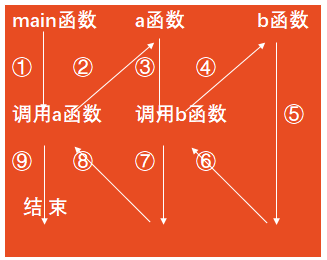
\includegraphics[scale=0.3]{main-a-b}
\column{0.5\textwidth}
\begin{lstlisting}[frame=leftline]
int a()
{
    int c; // 与main()中的c无关
    ...;
    c=b();// 函数调用
    ...;
    return c;
}
int b()
{
    ...;
    return 10;
}
\end{lstlisting}
\end{columns}
\medskip
\end{frame}


\begin{frame}[shrink,fragile]{例: 求4个整数中的最大者。}
\begin{columns}[T]
\column{0.54\textwidth}
\begin{lstlisting}
#include<stdio.h> 
int max2(int x,int y);
int max4(int a,int b,int c,int d); 
int main() // 主函数
{
   int a=b,c,d;
   scanf("%d%d%d%d",&a,&b,&c,&d);
   printf("较大者=%d\n", max4(a,b,c,d));
   printf("较大者=%d\n", max2(max2(a,b),max2(c,d))); // 等效
   return 0; 
}
\end{lstlisting}
\column{0.47\textwidth}
\begin{lstlisting}[frame=leftline]
// 定义函数
int max2(int x,int y) // 形式参数
{  
   int z;
   z=x>y ? x : y;
   return z; 
}
int max4(int a,int b,int c,int d)
{
  return max2(max2(a,b),max2(c,d));
}
\end{lstlisting}
\end{columns}
~\\
\end{frame}

\section{函数的递归调用}

\begin{frame}[shrink,fragile]{函数的递归调用}
\vspace{-0.2cm}
在调用一个函数的过程中又出现直接或间接地调用该函数本身,称为函数的递归调用。
\vspace{-0.4cm}
\begin{columns}[T]
\column{0.4\textwidth}
\begin{lstlisting}
// 递推公式: f(0)=0,f(1)=1, 
//     n>1: f(n)=n+f(n-1)
int f(int n) 
{
   int sum;
   if(n==0||n==1) sum=n;
   else sum=n+f(n-1); 
   return sum; 
}
\end{lstlisting}
\column{0.4\textwidth}
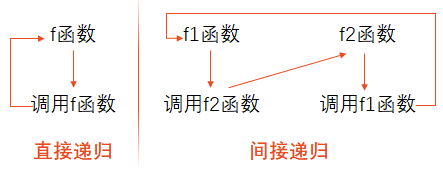
\includegraphics[scale=0.3]{recursion}
\vspace{-0.5cm}
\begin{align*}
f(1)&=1\\
f(2)&=2+f(1)=2+1\\
f(3)&=3+f(2)=3+2+1\\
f(n)&=n+f(n-1)=n+\underbrace{n-1+\cdots+2+1}_{f(n-1)}
\end{align*}
\end{columns}
切记不应出现无终止的递归调用。应是\textbf{有限次数的,有终止的递归调用},这可以用if语句来控制,只有在某一条件成立时才继续执行递归调用;否则就不再继续。
\end{frame}

\begin{frame}[shrink,fragile]{栈 --- 数据结构, push操作, 压入数据至栈顶}
系统内部自动维护一个称作``栈"的存储数据的空间。

栈是一种``先进后出(FILO)=后进先出(LIFO)"的数据结构。

向栈中存储数据操作称作push, 取出栈顶数据操作称作pop。

第一个push的数据,最后一个被pop.
\begin{columns}[T]
	\column{0.2\textwidth}<1->
	\begin{tabular}{|c|l}
		\cline{1-1}
		~&\\
		\cline{1-1}
		~&\\
		\cline{1-1}
		~&\\
		\cline{1-1} 
		\cellcolor{yellow}1&$\xleftarrow{top}$ \\ 
		\cline{1-1} 
	\end{tabular}\\ 
	栈[push(1)]
	\column{0.2\textwidth}<2->
	\begin{tabular}{|c|l}
		\cline{1-1}
		~&\\
		\cline{1-1}
		~&\\
		\cline{1-1} 
		\cellcolor{yellow}2 &$\xleftarrow{top}$ \\ 
		\cline{1-1} 
		1 &\\ 
		\cline{1-1}
	\end{tabular}\\ 
	栈[push(2)]
	\column{0.2\textwidth}<3->
	\begin{tabular}{|c|l}
		\cline{1-1}
		~&\\
		\cline{1-1}
		\cellcolor{yellow}3 &$\xleftarrow{top}$ \\ 
		\cline{1-1}
		2 &\\ 
		\cline{1-1}
		1 &\\ 
		\cline{1-1}
	\end{tabular}\\ 
	栈[push(3)]
	\column{0.2\textwidth}<4->
	\begin{tabular}{|c|l}
		\cline{1-1} 
		\cellcolor{yellow}4 &$\xleftarrow{top}$ \\ 
		\cline{1-1}
		3 &\\ 
		\cline{1-1}
		2 &\\ 
		\cline{1-1}
		1 &\\ 
		\cline{1-1}
	\end{tabular}\\ 
	栈[push(1)]
\end{columns}
\end{frame}

\begin{frame}[shrink,fragile]{栈 --- 数据结构, pop操作, 弹出栈顶数据}
系统内部自动维护一个称作``栈"的存储数据的空间。

栈是一种``先进后出(FILO)=后进先出(LIFO)"的数据结构。

向栈中存储数据操作称作push, 取出栈顶数据操作称作pop。

第一个push的数据,最后一个被pop.
\begin{columns}[T]
	\column{0.2\textwidth}<4->
	\begin{tabular}{|c|l}
		\cline{1-1}
		~&\\
		\cline{1-1}
		~&\\
		\cline{1-1}
		~&\\
		\cline{1-1} 
		\cellcolor{yellow}1&$\xleftarrow{top}$ \\ 
		\cline{1-1} 
	\end{tabular}\\ 
	栈[*pop=1]
	\column{0.2\textwidth}<3->
	\begin{tabular}{|c|l}
		\cline{1-1}
		~&\\
		\cline{1-1}
		~&\\
		\cline{1-1} 
		\cellcolor{yellow}2 &$\xleftarrow{top}$ \\ 
		\cline{1-1} 
		1 &\\ 
		\cline{1-1}
	\end{tabular}\\ 
	栈[*pop=2]
	\column{0.2\textwidth}<2->
	\begin{tabular}{|c|l}
		\cline{1-1}
		~&\\
		\cline{1-1}
		\cellcolor{yellow}3 &$\xleftarrow{top}$ \\ 
		\cline{1-1}
		2 &\\ 
		\cline{1-1}
		1 &\\ 
		\cline{1-1}
	\end{tabular}\\ 
	栈[*pop=3)]
	\column{0.2\textwidth}<1->
	\begin{tabular}{|c|l}
		\cline{1-1}
		\cellcolor{yellow}4 &$\xleftarrow{top}$ \\ 
		\cline{1-1} 
		3 &\\ 
		\cline{1-1}
		2 &\\ 
		\cline{1-1} 
		1 &\\ 
		\cline{1-1}
	\end{tabular}\\
	栈[*pop=4] 
\end{columns}
\end{frame}

\begin{frame}[shrink,fragile]{递归调用过程分析(push)}
\vspace{-0.3cm}
\begin{lstlisting}
// 递推公式: f(0)=0,f(1)=1, n>1: f(n)=n+f(n-1)
int f(int n) 
{
  int sum;
  if(n==0||n==1) sum=n;
  else sum=n+f(n-1); // 未完成的计算用"栈"存储起来(push)
  return sum; // 函数return前,从"栈"顶取数据,计算,直到"栈"空
}
\end{lstlisting}
\vspace{-0.3cm}
\begin{columns}[T]
\column{0.2\textwidth}<1->
\begin{tabular}{|c|l}
	\cline{1-1}
	~&\\
	\cline{1-1}
	~&\\
	\cline{1-1}
	~&\\
	\cline{1-1}
	\cellcolor{yellow}f(5)=5+f(4) & $\xleftarrow{top}$ \\ 
	\cline{1-1} 
\end{tabular}\\ 
栈[push(n=5)]
\column{0.2\textwidth}<2->
\begin{tabular}{|c|l}
	\cline{1-1}
	~&\\
	\cline{1-1}
	~&\\
	\cline{1-1} 
	\cellcolor{yellow}f(4)=4+f(3) & $\xleftarrow{top}$ \\ 
	\cline{1-1} 
	f(5)=5+f(4)& \\ 
	\cline{1-1} 
\end{tabular}\\ 
栈[push(n=4)]
\column{0.2\textwidth}<3->
\begin{tabular}{|c|l}
	\cline{1-1}
	~&\\
	\cline{1-1} 
	\cellcolor{yellow}f(3)=3+f(2)& $\xleftarrow{top}$ \\ 
	\cline{1-1} 
	f(4)=4+f(3)& \\ 
	\cline{1-1} 
	f(5)=5+f(4)& \\ 
	\cline{1-1} 
\end{tabular}\\ 
栈[push(n=3)]
\column{0.2\textwidth}<4->
\begin{tabular}{|c|l}
	\cline{1-1} 
	\cellcolor{yellow}f(2)=2+f(1)& $\xleftarrow{top}$ \\ 
	\cline{1-1} 
	f(3)=3+f(2)& \\ 
	\cline{1-1} 
	f(4)=4+f(3)& \\ 
	\cline{1-1} 
	f(5)=5+f(4)& \\ 
	\cline{1-1} 
\end{tabular}\\ 
栈[push(n=2)]
\end{columns}
~\\
\end{frame}

\begin{frame}[shrink,fragile]{递归调用过程分析(pop)}
\vspace{-0.3cm}
\begin{lstlisting}
// 递推公式: f(0)=0,f(1)=1, n>1: f(n)=n+f(n-1)
int f(int n) 
{
  int sum;
  if(n==0||n==1) sum=n;
  else sum=n+f(n-1); // 未完成的计算用"栈"存储起来(push)
  return sum; // 函数return前,从"栈"顶取数据,计算,直到"栈"空
}
\end{lstlisting}
\vspace{-0.3cm}
\begin{columns}[T]
	\column{0.25\textwidth}<4->
	\begin{tabular}{|c|l}
		\cline{1-1}
		~&\\
		\cline{1-1}
		~&\\
		\cline{1-1}
		~&\\ 
		\cellcolor{yellow}f(5)=5+f(4) & $\xleftarrow{top}$\\ 
		\cline{1-1} 
	\end{tabular}\\ 
	栈[pop(n=5)]\\
	f(5)=5+f(4)=15
	\column{0.25\textwidth}<3->
	\begin{tabular}{|c|l}
		\cline{1-1}
		~&\\
		\cline{1-1}
		~&\\
		\cline{1-1} 
		\cellcolor{yellow}f(4)=4+f(3) & $\xleftarrow{top}$ \\ 
		\cline{1-1} 
		f(5)=5+f(4) & \\ 
		\cline{1-1} 
	\end{tabular}\\ 
	栈[pop(n=4)]\\
	f(4)=4+f(3)=10
	\column{0.25\textwidth}<2->
	\begin{tabular}{|c|l}
		\cline{1-1}
		~&\\ 
		\cellcolor{yellow}f(3)=3+f(2) & $\xleftarrow{top}$ \\ 
		\cline{1-1} 
		f(4)=4+f(3) & \\ 
		\cline{1-1} 
		f(5)=5+f(4) & \\ 
		\cline{1-1} 
	\end{tabular}\\ 
	栈[pop(n=3)]\\
	f(3)=3+f(2)=6
	\column{0.25\textwidth}<1->
	\begin{tabular}{|c|l}
		\cline{1-1} 
		\cellcolor{yellow}f(2)=2+f(1) & $\xleftarrow{top}$ \\ 
		\cline{1-1} 
		f(3)=3+f(2) &\\ 
		\cline{1-1} 
		f(4)=4+f(3) & \\ 
		\cline{1-1} 
		f(5)=5+f(4) &\\ 
		\cline{1-1} 
	\end{tabular}\\ 
	栈[pop(n=2)]\\
	f(2)=2+f(1)=3
\end{columns}
~\\
\end{frame}

\begin{frame}[shrink]{例: age(n)}
有5个学生坐在一起,问第5个学生多少岁,他说比第4个学生大2岁。问第4个学生岁数,他说比第3个学生大2岁。问第3个学生,又说比第2个学生大2岁。问第2个学生,说比第1个学生大2岁。最后问第1个学生,他说是10岁。请问第5个学生多大。
~\\
\pause
\[ \text{第n个学生年龄 }
\begin{cases}
age(n)=10         & (n=1)\\
age(n)=age(n-1)+2 & (n>1) 
\end{cases}
\]
\end{frame}

\begin{frame}[shrink,fragile]{例: age(n), 递归调用过程分析(push)}
\vspace{-0.3cm}
\begin{lstlisting}
// 递推公式: age(1)=10; n>1: age(n)=age(n-1)
int age(int n) 
{
  int y;
  if(n==1) y=10;
  else y=age(n-1)+2; // 未完成的计算用"栈"存储起来(push)
  return y; // 函数return前,从"栈"顶取数据,计算,直到"栈"空
}
\end{lstlisting}
\vspace{-0.3cm}
\begin{columns}[T]
	\column{0.2\textwidth}<1->
	\begin{tabular}{|c|}
		\hline
		~\\
		\hline
		~\\
		\hline
		~\\ 
		\hline
		\rowcolor{yellow}age(5)=age(4)+2 \\ 
		\hline 
	\end{tabular}\\ 
	栈[push(n=5)]
	\column{0.2\textwidth}<2->
	\begin{tabular}{|c|}
		\hline
		~\\
		\hline
		~\\
		\hline 
		\rowcolor{yellow}age(4)=age(3)+2 \\ 
		\hline 
		age(5)=age(4)+2 \\ 
		\hline 
	\end{tabular}\\ 
	栈[push(n=4)]
	\column{0.2\textwidth}<3->
	\begin{tabular}{|c|}
		\hline
		~\\
		\hline 
		\rowcolor{yellow}age(3)=age(2)+2 \\ 
		\hline 
		age(4)=age(3)+2 \\ 
		\hline 
		\hline 
		age(5)=age(4)+2 \\ 
		\hline 
	\end{tabular}\\ 
	栈[push(n=3)]
	\column{0.2\textwidth}<4->
	\begin{tabular}{|c|}
		\hline 
		\rowcolor{yellow}age(2)=age(1)+2 \\ 
		\hline 
		age(3)=age(2)+2 \\ 
		\hline 
		age(4)=age(3)+2 \\ 
		\hline 
		\hline 
		age(5)=age(4)+2 \\ 
		\hline 
	\end{tabular}\\ 
	栈[push(n=2)]
\end{columns}
~\\
\end{frame}

\begin{frame}[shrink,fragile]{例: age(n), 递归调用过程分析(pop)}
\vspace{-0.3cm}
\begin{lstlisting}
// 递推公式: age(1)=10; n>1: age(n)=age(n-1)
int age(int n) 
{
  int y;
  if(n==1) y=10;
  else y=age(n-1)+2; // 未完成的计算用"栈"存储起来(push)
  return y; // 函数return前,从"栈"顶取数据,计算,直到"栈"空
}
\end{lstlisting}
\vspace{-0.3cm}
\begin{columns}[T]
\column{0.25\textwidth}<4->
\begin{tabular}{|c|}
	\hline 
	~\\
	\hline
	~\\
	\hline
	~\\
	\hline
	\rowcolor{yellow}age(5)=age(4)+2 \\ 
	\hline 
\end{tabular}\\ 
栈[pop(n=5)]\\
age(5)=age(4)+2=18
\column{0.25\textwidth}<3->
\begin{tabular}{|c|}
	\hline
	~\\
	\hline
	~\\
	\hline 
	\rowcolor{yellow}age(4)=age(3)+2 \\ 
	\hline 
	age(5)=age(4)+2 \\ 
	\hline 
\end{tabular}\\ 
栈[pop(n=4)]\\
age(4)=age(3)+2=16
\column{0.25\textwidth}<2->
\begin{tabular}{|c|}
	\hline 
	~\\
	\hline
	\rowcolor{yellow}age(3)=age(2)+2 \\ 
	\hline 
	age(4)=age(3)+2 \\ 
	\hline  
	age(5)=age(4)+2 \\ 
	\hline 
\end{tabular}\\ 
栈[pop(n=3)]\\
age(3)=age(2)+2=14
\column{0.25\textwidth}<1->
\begin{tabular}{|c|}
	\hline 
	\rowcolor{yellow}age(2)=age(1)+2 \\ 
	\hline 
	age(3)=age(2)+2 \\ 
	\hline 
	age(4)=age(3)+2 \\ 
	\hline  
	age(5)=age(4)+2 \\ 
	\hline 
\end{tabular}\\ 
栈[pop(n=2)]\\
age(2)=age(1)+2=12
\end{columns}
~\\
\end{frame}

\begin{frame}[shrink,fragile]{例: $n!$}
\vspace{-0.3cm}
\begin{tikzpicture}
\node[text width=\textwidth] (a) {
\begin{lstlisting}
double fac(int n) // n!较大,因此函数返回类型设置为double
{
   if(n==0 || n==1) return 1;
   else return n*fac(n-1);
}
int main()                   
{  
   printf("%.0lf\n",fac(2)); // 2
   printf("%.0lf\n",fac(3)); // 6
   printf("%.0lf\n",fac(4)); // 24
   printf("%.0lf\n",fac(20));// 2432902008176640000
   return 0;           
}           
\end{lstlisting}
};
\node[anchor=north east] at($(a.north east)+(-2.5,-2)$) {
	$n!=\begin{cases}
	1 &(n=0,1)\\
	n(n-1)! &(n>1)
	\end{cases}$
};
\end{tikzpicture}
\end{frame}

\begin{frame}[shrink,fragile]{例: 斐波那契数列 (double)}
\vspace{-0.3cm}
\begin{tikzpicture}
\node[text width=\textwidth] (a) {
\begin{lstlisting}
double F(int n) // Fn较大,因此函数返回类型设置为double
{
   if(n==0 || n==1) return 1;
   else return F(n-1)+F(n-2);
}
int main()                   
{  
   int i;
   for(i=0;i<20;i++)
   {
      printf("%d\t",(int)F(i));
      if((i+1)%4==0) printf("\n");
   } 
   return 0;           
}                            
\end{lstlisting}
};
\node[anchor=north east,fill=green,rounded corners] at($(a.north east)+(-1.5,-1)$) {
$\begin{cases}
F_n=1 &(n=0,1)\\
F_n=F_{n-1}+F_{n-2} &(n>1)
\end{cases}$
};
\end{tikzpicture}
\end{frame}

\begin{frame}[shrink,fragile]{例: 数字处理}
编写一个程序,从键盘输入一个非零整数n(0 < n <= 1000000000),对整数n进行如下处理:\\
将整数的各位数字取出来相加,如果结果是一位数则输出该数,否则重复上述过程,直到得到的结果为一位数,并输出该结果。\\
例如:n=456,变换过程如下\\
4+5+6=15\\
1+5=6\\
输出结果为6
\end{frame}

\begin{frame}[shrink,fragile]{例: 数字处理 --- 非递归实现}
\vspace{-0.3cm}
\begin{columns}[T]
\column{0.5\textwidth}
\begin{lstlisting}
#include<stdio.h>
int bitsSum(int a);
int main()
{
   int n,sum;
   scanf("%d",&n);
   while(1)
   {
      sum=bitsSum(n);
      if(sum<=9) break;//1位数字
      else n=sum; // 继续下一轮迭代 
    }
    printf("%d\n",sum); 
    return 0;
}
\end{lstlisting}
\column{0.4\textwidth}
\begin{lstlisting}[frame=leftline]
// 整数a的各位数字之和
int bitsSum(int a)
{
   int sum=0;
   while(a)
   {
      sum += a%10;
      a /= 10;
   }
   return sum;
}
\end{lstlisting}
\end{columns}
~\\
\end{frame}

\begin{frame}[shrink,fragile]{例: 数字处理 --- 递归实现}
\vspace{-0.4cm}
\begin{columns}[T]
\column{0.4\textwidth}
\begin{lstlisting}
#include<stdio.h>
int bitsSum(int a);
int bits1(int n);

int main()
{
   int n,sum=0;
   scanf("%d",&n);
   printf("%d\n",bits1(n)); 
   return 0;
} 
\end{lstlisting}
\column{0.6\textwidth}
\begin{lstlisting}[frame=leftline]
// 整数a的各位数字之和
int bitsSum(int a)
{
   int sum;
   if(a==0) sum=0;  
   else sum=bitsSum(a/10)+a%10; //递归
   return sum;
}
// 确保最后是1位数字
int bits1(int n)
{
   int result;
   result=bitsSum(n);
   if(result>9) result=bits1(result);//递归
   return result; 
}
\end{lstlisting}
\end{columns}
~\\
\end{frame}

\begin{frame}[shrink,fragile]{例: 二进制输出(正序)}
\vspace{-0.5cm}
\begin{columns}[T]
\column{0.6\textwidth}
\begin{lstlisting}
void to_binary(unsigned long n)
{
	int r;
	r=n%2;//01001011
	// push(先计算的二进制位r)
	if(n>=2) to_binary(n/2); 
	// pop(后进先出FILO=先进后出FILO) 
	putchar('0'+r);//11010010
} 
int main()
{
	// 无符号长整型, 可赋值10进制数
	unsigned long x=0XD2; //11010010
	scanf("%x",&x); //十六进制输入
	//等效10进制无符号长整型 
	//scanf("%uld",&x);  
	to_binary(x);
	putchar('\n'); 
	return 0;
}
\end{lstlisting}

\column{0.75\textwidth}
~\\
以\lstinline|x=0XD2=|$(11010010)_2$为例,分析递归过程。 \\
(1) \lstinline|r=n%2;|\\
计算顺序$2^0,2^1,\dots,2^7$\\
\begin{tabular}{|c|c|c|c||c|c|c|c|}
	\hline 
	$2^0$& $2^1$ & $2^2$ & $2^3$ & $2^4$ & $2^5$ & $2^6$ & $2^7$  \\ 
	\hline 
	0 & 1 & 0 & 0 & 1 & 0 & 1 & 1 \\ 
	\hline 
\end{tabular}

\vspace{0.5cm}
(2) \lstinline|to_binary(n/2);|\\
push(先计算的r),栈顶(top,最左端), 栈底(bottom,最右端)\\ 
\begin{tabular}{|c|c|c|c||c|c|c|c|}
	\hline 
	$2^7$& $2^6$ & $2^5$ & $2^4$ & $2^3$ & $2^2$ & $2^1$ & $2^0$
	\\ 
	\hline 
	1 & 1 & 0 & 1 & 0 & 0 & 1 & 0 \\ 
	\hline 
\end{tabular}  

\vspace{0.5cm}
(3) \lstinline|putchar('0'+r);|\\
pop(后进先出), 栈顶元素先出,栈底元素最后出\\
\begin{tabular}{|c|c|c|c||c|c|c|c|}
	\hline 
	$2^7$& $2^6$ & $2^5$ & $2^4$ & $2^3$ & $2^2$ & $2^1$ & $2^0$
	\\ 
	\hline 
	1 & 1 & 0 & 1 & 0 & 0 & 1 & 0 \\ 
	\hline 
\end{tabular}  
\end{columns}
~\\
\end{frame}

\begin{frame}[shrink,fragile]{例: 二进制输出(倒序)}
\vspace{-0.5cm}
\begin{columns}[T]
\column{0.6\textwidth}
\begin{lstlisting}
void to_binary(unsigned long n)
{
	int r;
	r=n%2;//01001011
	putchar('0'+r);//01001011
	// push(先计算的二进制位r)
	if(n>=2) to_binary(n/2); 
} 
int main() // 与正序一致
{
	// 无符号长整型
	unsigned long x=0XD2; //11010010
	scanf("%x",&x); //十六进制输入
	//等效10进制无符号长整型 
	//scanf("%uld",&x); 
	to_binary(x);
	putchar('\n'); 
	return 0;
}
\end{lstlisting}
\column{0.75\textwidth}
	~\\
	以\lstinline|x=0XD2=|$(11010010)_2$为例,分析递归过程。 \\
	(1) \lstinline|r=n%2; putchar('0'+r); |\\
	计算顺序(同输出顺序)$2^0,2^1,\dots,2^7$\\
	\begin{tabular}{|c|c|c|c||c|c|c|c|}
		\hline 
		$2^0$& $2^1$ & $2^2$ & $2^3$ & $2^4$ & $2^5$ & $2^6$ & $2^7$  \\ 
		\hline 
		0 & 1 & 0 & 0 & 1 & 0 & 1 & 1 \\ 
		\hline 
	\end{tabular}
	
	\vspace{0.5cm}
	(2) \lstinline|to_binary(n/2);|\\
	push(先计算的r),栈顶(top,最左端), 栈底(bottom,最右端)\\ 
	\begin{tabular}{|c|c|c|c||c|c|c|c|}
		\hline 
		$2^7$& $2^6$ & $2^5$ & $2^4$ & $2^3$ & $2^2$ & $2^1$ & $2^0$
		\\ 
		\hline 
		1 & 1 & 0 & 1 & 0 & 0 & 1 & 0 \\ 
		\hline 
	\end{tabular}  
	
	\vspace{0.5cm}
	(3) pop(后进先出), 栈顶元素先出,栈底元素最后出\\
	\begin{tabular}{|c|c|c|c||c|c|c|c|}
		\hline 
		$2^7$& $2^6$ & $2^5$ & $2^4$ & $2^3$ & $2^2$ & $2^1$ & $2^0$
		\\ 
		\hline 
		1 & 1 & 0 & 1 & 0 & 0 & 1 & 0 \\ 
		\hline 
	\end{tabular}  
\end{columns}
~\\
\end{frame}

\begin{frame}[shrink,fragile]{例: 生成正整数对应的二进制字符串}
\vspace{-0.1cm}
\begin{tikzpicture}
\node[text width=0.75\textwidth,rounded corners,draw] (a) {
	\vspace{-0.3cm}
	\begin{lstlisting}
		void to_binary(int n)
		{
			int r;
			r=n%2; 
			// push(先计算的二进制位r)
			if(n>=2) to_binary(n/2); 
			// pop(后进先出FILO=先进后出FILO) 
			putchar('0'+r);//每次pop输出一位字符: 1111011
		} 
	    int main()
	    {
	    	to_binary(123);
	    	// 测试
	    	printf("%X\n",123) // 7B ==> $(\underbrace{111}_7\underbrace{1011}_B)_2$ 
	    }
	\end{lstlisting}
};
\node[anchor=west,text width=0.35\textwidth,rounded corners,fill=green] (b) at($(a.east)+(0.2cm,0)$) {
	分析上例的核心代码, 由此得到设计思路:
	
	替换函数to\_binary的最后一条输出语句,设计函数catC(char s[], char c), 连接字符c至字符串s, 即是所求的二进制字符串。
};
\end{tikzpicture}
\end{frame}

\begin{frame}[shrink,fragile]{例: 生成正整数对应的二进制字符串, 设计函数catC}
\vspace{-0.1cm}
\begin{tikzpicture}
%% 左上
\node[text width=0.5\textwidth,rounded corners,draw] (a) {
	\vspace{-0.3cm}
	\begin{lstlisting}
	void catC(char s[], char c)
	{
		int len=0;
		for(; s[len]!='\0';len++) ;
		s[len]=c; s[len+1]='\0';
	}
	\end{lstlisting}
};
%% 右上
\node[anchor=north west,text width=0.5\textwidth,rounded corners,draw] (b) at(a.north east){
	\vspace{-0.3cm}
	\begin{lstlisting}
	void catC(char s[], char c)
	{
		int i,len=0;
		for(i=0; s[i]!='\0';i++)len++;
		s[len]=c; s[len+1]='\0';
	}
	\end{lstlisting}	
};
%% 左下
\node[anchor=north west,text width=0.5\textwidth,rounded corners,draw] (c) at(a.south west){
	\vspace{-0.3cm}
	\begin{lstlisting}
	void catC(char s[], char c)
	{
		int len;
		len=strlen(s);
		s[len]=c; s[len+1]='\0';
    } 
	\end{lstlisting}	
};
%% 左下下
\node[anchor=north west,text width=0.5\textwidth,rounded corners,fill=green,font=\small] at(c.south west){
	等效的四种编码方式, 要求s以\lstinline|'\0'|结尾。
};

%% 右下
\node[anchor=north west,text width=0.5\textwidth,rounded corners,draw] (d) at(b.south west){
	\vspace{-0.3cm}
	\begin{lstlisting}
	void catC(char s[], char c)
	{
		char str[2];
		// 构造以'\0'结尾的str字符串 
		str[0]=c; str[1]='\0';
		strcat(s,str); // 连接s,str 
	}
	\end{lstlisting}	
};
\end{tikzpicture}
\end{frame}

\begin{frame}[shrink,fragile]{例: 生成正整数对应的二进制字符串, 测试函数catC}
\vspace{-0.1cm}
\begin{center}
\begin{tikzpicture}
\node[text width=0.65\textwidth,rounded corners,draw] (a) {
	\vspace{-0.3cm}
	\begin{lstlisting}
	void catC(char s[], char c)
	{
		int len=0;
		for(; s[len]!='\0';len++) ;
		s[len]=c; s[len+1]='\0';
	}
	int main() // 测试任意一种定义方式
	{
		char s[81]="";//初始化为以'\0'结尾的空字符串
		// char s[81]={'\0'}; // 等效
		catC(s,'1');  // 连接, s[1]='\0' 
		puts(s); // 1
		catC(s,'2');  // 连接, s[2]='\0'
		puts(s); // 12 
	} 
	\end{lstlisting}
};

\end{tikzpicture}
\end{center}
\end{frame}

\begin{frame}[shrink,fragile]{例: 生成正整数对应的二进制字符串, 完整代码}
\vspace{-0.1cm}
\begin{tikzpicture}
\node[text width=0.55\textwidth,rounded corners] (a) {
\vspace{-0.3cm}
\begin{lstlisting}
// 把字符c连接至字符串s, 要求s以'\0'结尾. 
void catC(char s[], char c)
{	int len=0;
	for(; s[len]!='\0';len++) ;
	s[len]=c; s[len+1]='\0';
}
// s存放n对应的二进制字符串,以'\0'结尾. 
// 返回字符串s的长度.
int to_binary(int n, char s[])
{	int r;
	r=n%2; 
	// push(先计算的二进制位r)
	if(n>=2) to_binary(n/2, s); 
	// pop(后进先出FILO=先进后出FILO) 
	catC(s,'0'+r);  // 连接
	return strlen(s);
} 	
\end{lstlisting}
};

\node[anchor=north west,text width=0.65\textwidth,rounded corners] (b) at(a.north east){
\vspace{-0.3cm}
\begin{lstlisting}
int main() // 测试
{
	char s[81]="";//初始化为以'\0'结尾的空字符串
	// char s[81]={'\0'}; // 等效
	int n=123;
	//scanf("%d",&n); // 输入一个正整数
	// 调用测试
	printf("%d\n",to_binary(n,s)); // 7
	puts(s); // 1111011
	// 验证
	printf("%X\n",123) // 7B ==> $(\underbrace{111}_7\underbrace{1011}_B)_2$ 
} 
\end{lstlisting}
};

\draw[dashed,red] (a.north east) -- (a.south east);
\end{tikzpicture}
\end{frame}

\begin{frame}{例: Hanoi(汉诺)塔问题}
\vspace{-0.4cm}
古代有一个梵塔,塔内有3个座A,B,C。开始时A座上有64个盘子,盘子大小不等,大的在下,小的在上。有一个老和尚想把这64个盘子从A座移到C座,但规定每次只允许移动一个盘,且在移动过程中在3个座上都始终保持大盘在下,小盘在上。在移动过程中可以利用B座。要求编程序输出移动盘子的步骤。\\
~\\
\centering
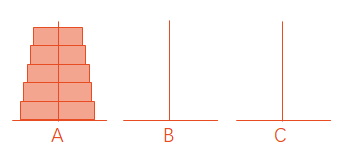
\includegraphics[scale=0.4]{Hanoi}
\end{frame}

\begin{frame}[shrink]{例: Hanoi(汉诺)塔问题---解题思路}
\vspace{-0.4cm}
\begin{tikzpicture}
\node[text width=\textwidth] (a) {
	\begin{itemize}
		\item 老和尚想: 假如有第2个和尚将上面63个盘子从A座移到B座。我就能将64个盘子从A座移到C座。
			\begin{enumerate}
			\item 命令第2个和尚将63个盘子从A座移到B座;
			\item 自己将1个盘子(最底下的、最大的盘子)从A座移到C座;
			\item 再命令第2个和尚将63个盘子从B座移到C座。
			\end{enumerate}
		\item 第2个和尚想: 假如有第3个和尚能将上面62个盘子从A座移到C座,我就能将63个盘子从A座移到B座。
			\begin{enumerate}
			\item 命令第3个和尚将62个盘子从A座移到C座;
			\item 自己将1个盘子从A座移到B座;
			\item 再命令第3个和尚将62个盘子从C座移到B座。
			\end{enumerate}
		\item $\cdots$
	\end{itemize}
};
\node[anchor=south east,text width=.25\textwidth] at(a.south east) {
	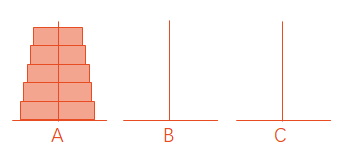
\includegraphics[scale=0.25]{Hanoi}\\
	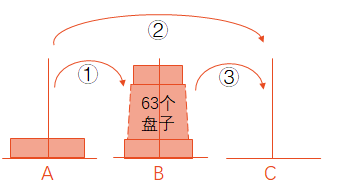
\includegraphics[scale=0.3]{Hanoi-1}
};
\end{tikzpicture}
\end{frame}

\begin{frame}[shrink]{例: Hanoi(汉诺)塔问题---解题思路(3层)}
\vspace{-0.4cm}
\begin{columns}[T]
	\column{0.6\textwidth}
	\begin{itemize}
		\item 将A座的3个盘子移到C座, 分3步:
		\begin{enumerate}
			\item 将A上2个盘子移到B\textbf{(借助C座)}。
			\item 将A上1个盘子移到C\textbf{(直接实现)}。
			\item 将B上2个盘子移到C\textbf{(借助A座)}。
		\end{enumerate}
	    \item 分解第1步: 将A上的2个盘子移到B:
	    \begin{enumerate}
	    	\item 将A上1个盘子移到C\textbf{(借助C座)}。
	    	\item 将A上1个盘子移到B。
	    	\item 将C上1个盘子移到B。
	    \end{enumerate}
        \item 分解第3步: 将B座的2个盘子移到C座:
        \begin{enumerate}
        	\item 将B上1个盘子移到A\textbf{(借助A座)}。
        	\item 将B上1个盘子移到C。
        	\item 将A上1个盘子移到C。
        \end{enumerate}
	\end{itemize}
	\column{0.4\textwidth}
	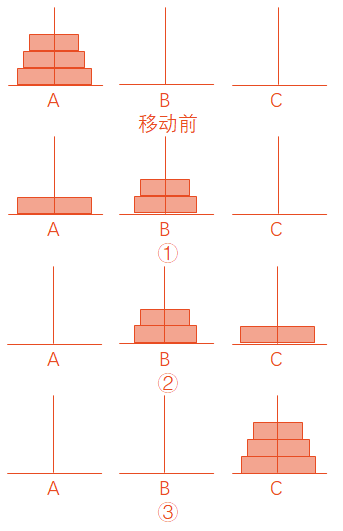
\includegraphics[scale=0.3]{Hanoi-2}
\end{columns}
~\\
\end{frame}

\begin{frame}[shrink,fragile]{例: Hanoi(汉诺)塔问题---解}
\vspace{-0.4cm}
\begin{columns}[T]
\column{0.4\textwidth}
\begin{lstlisting}
int main()
{
   int n=3;
   scanf("%d",&n);
   //n个盘由'A'移到'C',借助'B'
   hanoi(n,'A','B','C');
   return 0;
}
void move(char one,char two)
{
 printf("%c->%c\n",one,two);
}
\end{lstlisting}
\column{0.65\textwidth}
\begin{lstlisting}[frame=leftline]
//将n个盘从one移到three,借助two
void hanoi(int n,char one,char two,char three)
{
   if(n==1) move(one,three); 
   else
   {
      //n-1盘从one移到two,借three
      hanoi(n-1,one,three,two); 
      //将1个盘从one移到three
      move(one,three); 
      //n-1盘从two移到three,借one
      hanoi(n-1,two,one,three); 
   }
}
\end{lstlisting}
\end{columns}
~\\
\end{frame}

\begin{frame}[shrink, fragile]%{例: Hanoi(汉诺)塔问题---分析代码(3层)}
\vspace{-0.4cm}
\begin{columns}[T]
\column{0.4\textwidth}
	\begin{itemize}
		\small
		\item 将A座的3个盘子移到C座, 分3步:
		\begin{enumerate}
			\scriptsize
			\item 将A上2个盘子移到B\textbf{(借C)}。
			\item 将A上1个盘子移到C\textbf{(直接)}。
			\item 将B上2个盘子移到C\textbf{(借A)}。
		\end{enumerate}
		\item 分解第1步: 将A上的2个盘子移到B:
		\begin{enumerate}\scriptsize
			\item 将A上1个盘子移到C\textbf{(借C)}。
			\item 将A上1个盘子移到B。
			\item 将C上1个盘子移到B。
		\end{enumerate}
		\item 分解第3步: 将B座的2个盘子移到C座:
		\begin{enumerate}\scriptsize
			\item 将B上1个盘子移到A\textbf{(借A)}。
			\item 将B上1个盘子移到C。
			\item 将A上1个盘子移到C。
		\end{enumerate}
	\end{itemize}
\column{0.65\textwidth}
\begin{lstlisting}[frame=leftline]
//将n个盘从one移到three,借助two
void hanoi(int n,char one,char two,char three)
{
  // 递归终止条件, 出栈pop(2,...,n-1,n), 回归,回溯
  if(n==1) move(one,three); 
  else
  { //压栈push(n,n-1,n-2,...2)
    //n-1盘从one移到two,借three
    hanoi(n-1,one,three,two); 
    //将1个盘从one移到three
    move(one,three); 
    //n-1盘从two移到three,借one
    hanoi(n-1,two,one,three);
  }
}
\end{lstlisting}
\end{columns}
\textcolor{blue}{$A\to C,A\to B,C\to B,A\to C,B\to A,B\to C,A\to C$}\\
\end{frame}

\begin{frame}[shrink,fragile]{递归小结}
\vspace{-0.4cm}
\begin{itemize}
	\item 递归函数必须满足两个条件:
	\begin{enumerate}
		\item 在每一次调用自己时,必须是(在某种意义上)更接近于解;
		\item 必须有一个终止处理的语句。
	\end{enumerate}
    \item 递归能够解决的问题:
    \begin{enumerate}
    	\item 数据的定义是按递归定义的。如Fibonacci函数。
    	\item 问题解法按递归算法实现。如Hanoi问题。
    	\item 数据的结构形式是按递归定义的。如二叉树、广义表等。
    \end{enumerate}
	\item 使用递归的关键在于将问题分解为小部分,递归不能永远进行下去,因为它总是以最小可能性问题结束,
	\item 递归函数的优点是定义简单,逻辑清晰,但是代码难于理解。
	\item 理论上,所有的递归函数都可以写成循环的方式,但循环逻辑不如递归清晰。
	\item 层次越深, 调用栈(内存)越大, 效率越低, 并且可能会溢出。因此, 能用循环解决的问题, 尽量不要用递归。
\end{itemize}
\end{frame}

\section{局部变量和全局变量}

\begin{frame}[shrink,fragile]{定义在函数内部或复合语句中的变量: 局部变量}
局部变量的\textbf{作用域}是从定义语句开始至函数或复合语句结束,不会影响作用域以外的同类型的同名变量值。 
\vspace{-0.3cm}
\begin{columns}[T]
\column{0.5\textwidth}
\begin{lstlisting}
// 各函数中的局部变量, 不会相互影响。
float f1(folat a) 
{
   float c; // 本函数局部变量
   ....;
}
float f2(float a)
{ 
   float c; // 本函数局部变量
   ....;
}
int main()
{
   float c=10,d; // 本函数局部变量
   d=f1(c); d=f2(d);
}
\end{lstlisting}
\column{0.7\textwidth}
\begin{lstlisting}[frame=leftline]
// 各复合语句中的局部量, 不会相互影响。
float f1(folat a) 
{
   float c; // 本函数局部变量
   for(int i=0;i<10;i++) // i: for复合语句中的局部变量
   {
     int t; // 复合语句中的局部变量 
     ....
   }
   if(c>10)
   {
     int t; // 复合语句中的局部变量 
     ....
   }
   ...
}
\end{lstlisting}
\end{columns}
~\\
\end{frame}

\begin{frame}[shrink,fragile]{形式参数被当作本函数的局部变量}
形式参数被当作本函数的局部变量,因此它不会影响实际参数的值。
\vspace{-0.3cm}
\begin{columns}[T]
\column{0.6\textwidth}
\begin{lstlisting}
float f1(folat a) 
{
  float c;//函数内部的局部变量不得与形式参数同名
  a=30; // 改变形式参数的值不会影响实际参数的值
}
int main()
{
   float c=10,d;//主函数局部变量
   d=f1(c);//f1函数对形参的改变不会影响实参c的值
   float x[2]={0.1,0.2}; 
   f2(x); // 函数内部可以改变数组元素的值
   printf("%f,%f,%f\n",c,x[0],x[1]); // 10,10.1,10.2  
}
\end{lstlisting}
\column{0.55\textwidth}
\begin{lstlisting}[frame=leftline]
//函数内部可以改变数组元素的值,但是对地址的改变不会影响实参的地址
//形式参数的数组名是地址变量, 不是常量.
//回忆: int m[5]; // 数组名是地址常量.
float f2(folat a[]) 
{
  //对数组元素的改变,就是对实参数组元素的改变
  a[0]=10.1;
  a[1]=10.2;
  //对数组名(地址)的改变, 不会影响实参的地址。
  a=a+1; 
}
\end{lstlisting}
\end{columns}
~\\
\end{frame}

\begin{frame}[shrink,fragile]{定义在函数外部的变量: 全局变量}
与模块化函数封装思想冲突,不推荐使用。全局变量的作用域是从定义语句开始至该文件结束,会影响作用域内的同类型的同名变量值。 
\begin{lstlisting}
int g=0; // 全局变量
float f1(folat a) 
{
  g=10; // 改变全局变量的值
}
float f2(float a)
{ 
  g=20; // 改变全局变量的值
}
int main()
{
   g=30; // 改变全局变量的值
}
\end{lstlisting}
\end{frame}




 % ch7, 函数,定义,声明,调用,值传递,地址传递,模块化设计
%%%%%%%%%%% lecture-13: 第14次课基本概念, 第15次课,实例分析,第2次机试练习ISBN讲解
%%%%%%%%%%%%%%%%%%%%%%%%%% lecture-14
%\begin{frame}[shrink]
%  \frametitle{lecture-14 主要内容}
%  \framesubtitle{善于利用指针}
%  %\tableofcontents[hideallsubsections]
%  \tableofcontents
%\end{frame}

\section{指针就是指向变量存储单元(首)地址的变量}

\begin{frame}[shrink,fragile]{指针就是指向变量存储单元(首)地址的变量}
\vspace{-0.4cm}
\begin{columns}[T]
\column{0.87\textwidth}
\small
\begin{itemize}
\item 在程序中定义的各个变量, 在对程序进行编译时,系统就会给每个变量分配一个存储单元。
\item 基本存储单元是一个字节(byte)。
\item 根据变量类型,系统分配相应长度的存储单元, 其长度是字节的整数倍。
\item 不同的编译器,给变量分配的存储空间可能会有所不同。sizeof(类型), 可获得该编译器给相应类型的变量分配的存储空间大小。
\item 指针就是指向目标变量存储单元(首)地址的变量。
\end{itemize}
\begin{lstlisting}
char c;//分配1个存储单元, 即1个字节
int  a;//分配2个存储单元, 即2个字节(大多数是4个字节)
float f;//分配4个存储单元, 即4个字节
double d; //分配8个存储单元, 即8个字节
printf("%d,%d,%d,%d\n",sizeof(char),sizeof(int),sizeof(float),sizeof(double)); 
// 1,4,4,8
\end{lstlisting}
\column{0.3\textwidth}
\small
\begin{tabular}{|c|c|c|}
	\hline 
	\textbf{变量名} & \textbf{地址} & \textbf{内容} \\ 
	\hline 
	c & \textcolor{blue}{2000} & `A' \\ 
	\hline 
	& $\dots$ &  \\ 
	\hline 
	\multirow{2}{*}{a} & \textcolor{blue}{3000} & \multirow{2}{*}{20} \\ \cline{2-2} 
	%\hline 
	& 3001 &  \\ 
	\hline 
	& $\dots$ &  \\ 
	\hline 
	\multirow{4}{*}{f} & \textcolor{blue}{4000} & \multirow{4}{*}{10.2}  \\ \cline{2-2} 
	%\hline 
	& 4001 &  \\ \cline{2-2}
	%\hline 
	& 4002 &  \\ \cline{2-2}
	%\hline 
	& 4003 &  \\ 
	\hline 
	& $\dots$ &  \\ 
	\hline 
	\multirow{4}{*}{d} & \textcolor{blue}{5000} & \multirow{4}{*}{20.8} \\ \cline{2-2}
	%\hline 
	& 5001 &  \\ \cline{2-2}
	%\hline 
	& 5002 &  \\ \cline{2-2}
	%\hline 
	& 5003 &  \\ \cline{2-2}
	\hline 
\end{tabular} 
\end{columns}
\medskip
\end{frame}

\section{定义指针变量: int *p;}

\begin{frame}[shrink,fragile]{定义指针变量: int *p;}
\textbf{\textcolor{blue}{指针就是指向变量存储单元(首)地址的变量。}}\\
\medskip
\lstinline|数据类型 *指针变量名; //数据类型表示指针指向目标变量类型,*表示其后的变量是指针变量|
\begin{lstlisting}
int *pa; // 定义指向整数类型变量的指针变量pa, *表示其后的变量是指针变量
char *pc; // 定义指向字符类型变量的指针变量pc
float *pf; // 定义指向单精度浮点类型变量的指针变量pf
double *pd; // 定义指向双精度浮点类型变量的指针变量pd
\end{lstlisting}
\begin{block}{特别注意}
	以上定义了各个指针变量,但是还没有设置指针指向的目标变量。未设置目标变量前的指针变量, 是一个``无用"的变量, 此时定义的指针变量仅说明了将来的目标变量的数据类型。
\end{block}
\end{frame}

\begin{frame}[shrink,fragile]{设置指针变量指向的目标变量}
\vspace{-0.4cm}
\begin{columns}[T]
\column{0.8\textwidth}
\textbf{\textcolor{blue}{地址运算符\&, 可获得变量在内存中的(首)地址。}}
\begin{lstlisting}
// 定义指针变量pa, 并初始化pa指向变量a
int a=20,*pa=&a; 
// 定义指针变量pc, 并初始化pc指向变量c
char c='A',*pc=&c; 
// 定义指针变量pf, 并初始化pf指向变量f
float f=10.2,*pf=&f; 
// 定义指针变量pd, 并初始化pd指向变量d
double d=20.8,*pd=&d;

int b=30,*p; 

// 根据需要,可以随时设置指针指向的目标变量
p=&b; 
// 改变pa的指向
pa=p; // 或 pa=&b;
\end{lstlisting}
\column{0.3\textwidth}
\small
\begin{tabular}{|c|c|c|c|}
	\hline 
	\textbf{变量名} & \textbf{指针} &\textbf{地址} & \textbf{内容} \\ 
	\hline 
	c & pc $\to$& \textcolor{blue}{2000} & `A' \\ 
	\hline 
	& & $\dots$ &  \\ 
	\hline 
	\multirow{2}{*}{a} &  pa $\to$ & \textcolor{blue}{3000} & \multirow{2}{*}{20} \\ \cline{3-3} 
	%\hline 
	& & 3001 &  \\ 
	\hline 
	& & $\dots$ &  \\ 
	\hline 
	\multirow{4}{*}{f} &  pf $\to$ & \textcolor{blue}{4000} & \multirow{4}{*}{10.2}  \\ \cline{3-3} 
	%\hline 
	& & 4001 &  \\ \cline{3-3}
	%\hline 
	& & 4002 &  \\ \cline{3-3}
	%\hline 
	& &4003 &  \\ 
	\hline 
	& & $\dots$ &  \\ 
	\hline 
	\multirow{4}{*}{d} &  pd $\to$ & \textcolor{blue}{5000} & \multirow{4}{*}{20.8} \\ \cline{3-3}
	%\hline 
	& & 5001 &  \\ \cline{3-3}
	%\hline 
	& & 5002 &  \\ \cline{3-3}
	%\hline 
	& & 5003 &  \\ 
	\hline 
\end{tabular} 
\end{columns}
\medskip
\end{frame}

\section{变量的直接访问与间接访问}

\begin{frame}[shrink,fragile]{变量的直接访问}
\vspace{-0.4cm}
\begin{columns}[T]
\column{0.85\textwidth}
\begin{itemize}
	\item \textbf{\textcolor{blue}{直接访问:}} 通过变量名访问(读写)存储单元的内容(变量的值)
	\item 此前的程序, 均采用直接访问的形式, 读写变量的值。
\end{itemize}
\begin{lstlisting}
char c; // 分配1个存储单元, 即1个字节
int  a; // 分配2个存储单元, 即2个字节(大多数是4个字节)
float f; // 分配4个存储单元, 即4个字节
double d; // 分配8个存储单元, 即8个字节
// 直接访问
// "写" 变量的值
c='A';
a=20;
f=10.2;
d=20.8;
// "读"变量的值
printf("%c,%d,%f,%lf\n",c,a,f,d);
\end{lstlisting}
\column{0.3\textwidth}
\small
\begin{tabular}{|c|c|c|}
	\hline 
	\textbf{变量名} & \textbf{地址} & \textbf{内容} \\ 
	\hline 
	c & \textcolor{blue}{2000} & `A' \\ 
	\hline 
	& $\dots$ &  \\ 
	\hline 
	\multirow{2}{*}{a} & \textcolor{blue}{3000} & \multirow{2}{*}{20} \\ \cline{2-2} 
	%\hline 
	& 3001 &  \\ 
	\hline 
	& $\dots$ &  \\ 
	\hline 
	\multirow{4}{*}{f} & \textcolor{blue}{4000} & \multirow{4}{*}{10.2}  \\ \cline{2-2} 
	%\hline 
	& 4001 &  \\ \cline{2-2}
	%\hline 
	& 4002 &  \\ \cline{2-2}
	%\hline 
	& 4003 &  \\ 
	\hline 
	& $\dots$ &  \\ 
	\hline 
	\multirow{4}{*}{d} & \textcolor{blue}{5000} & \multirow{4}{*}{20.8} \\ \cline{2-2}
	%\hline 
	& 5001 &  \\ \cline{2-2}
	%\hline 
	& 5002 &  \\ \cline{2-2}
	%\hline 
	& 5003 &  \\ 
	\hline 
\end{tabular} 
\end{columns}
\medskip
\end{frame}

\begin{frame}[shrink,fragile]{变量的间接访问}
\vspace{-0.4cm}
\begin{columns}[T]
\column{0.85\textwidth}
\begin{itemize}
	\item \textbf{\textcolor{blue}{间接访问:}} 通过变量的(首)地址访问(读写)存储单元的内容(变量的值)
	\item *指针变量, \textbf{\textcolor{blue}{间接访问运算符*}}, 表示读写指针的目标变量值
\end{itemize}
\vspace{-0.2cm}
\begin{lstlisting}
// 定义指针变量,并初始化, 指向特定的变量地址
char c, *pc=&c; //pc是指向char类型变量的指针变量
int  a, *pa=&a; //pa是指向char类型变量的指针变量
float f, *pf=&f; //pf是指向char类型变量的指针变量
double d, *pd=&d; //pd是指向char类型变量的指针变量
// 间接访问
// "写" 变量的值
*pc='A'; // 不要忘记前面的*, 否则成为改变指针指向的语句。
*pa=20;
*pf=10.2;
*pd=20.8;
// "读"变量的值
printf("%c,%d,%f,%lf\n",*pc,*pa,*pf,*pd);
\end{lstlisting}
\column{0.3\textwidth}
\small
\begin{tabular}{|c|c|c|c|}
	\hline 
	\textbf{变量名} & \textbf{指针} &\textbf{地址} & \textbf{内容} \\ 
	\hline 
	c & pc $\to$& \textcolor{blue}{2000} & `A' \\ 
	\hline 
	& & $\dots$ &  \\ 
	\hline 
	\multirow{2}{*}{a} &  pa $\to$ & \textcolor{blue}{3000} & \multirow{2}{*}{20} \\ \cline{3-3} 
	%\hline 
	& & 3001 &  \\ 
	\hline 
	& & $\dots$ &  \\ 
	\hline 
	\multirow{4}{*}{f} &  pf $\to$ & \textcolor{blue}{4000} & \multirow{4}{*}{10.2}  \\ \cline{3-3} 
	%\hline 
	& & 4001 &  \\ \cline{3-3}
	%\hline 
	& & 4002 &  \\ \cline{3-3}
	%\hline 
	& &4003 &  \\ 
	\hline 
	& & $\dots$ &  \\ 
	\hline 
	\multirow{4}{*}{d} &  pd $\to$ & \textcolor{blue}{5000} & \multirow{4}{*}{20.8} \\ \cline{3-3}
	%\hline 
	& & 5001 &  \\ \cline{3-3}
	%\hline 
	& & 5002 &  \\ \cline{3-3}
	%\hline 
	& & 5003 &  \\ 
	\hline 
\end{tabular} 
\end{columns}
\medskip
\end{frame}

\begin{frame}[shrink,fragile]{指针变量使用(间接访问)前,必须有指向。}
\vspace{-0.4cm}
\begin{lstlisting}
// 注意: 指针变量使用前,必须有指向
float *p;
*p=10.2; // 错!!! p没有设置指向的目标变量,即p未赋值,间接访问是错误的。

float f;
p=&f;
*p=10.2; // 合法

int a, *pa;
scanf("%d",pa); // 错!!! pa没有设置指向的目标变量
pa=&a; // 设置pa指向a
scanf("%d",pa); // pa有指向了, 正确
scanf("%d",&a); // 等效
printf("%d,%d\n",a,*pa); // 输出相同的值
\end{lstlisting}
\end{frame}

\begin{frame}[shrink,fragile]{例: 交换两个指针变量的值(地址, 指向)}
\vspace{-0.4cm}
\begin{lstlisting}
int a=10, *pa=&a, b=20, *pb=&b;
int *tmp;
if(a<b) // 不交换a,b的值, 交换pa,pb的指向
{
  tmp=pa;
  pa=pb;
  pb=tmp;
}
printf("%d,%d,%d,%d\n",a,b,*pa,*pb); // 10,20,20,10

// 或者, 不使用中间变量
if(a<b) // 不交换a,b的值, 交换pa,pb的指向
{
  pa=&b;
  pb=&a;
}
printf("%d,%d,%d,%d\n",a,b,*pa,*pb); // 10,20,20,10
\end{lstlisting}
\end{frame}

\section{地址传递与值传递}

\begin{frame}[shrink,fragile]{\small 指针变量作为函数参数(地址传递, 形参和实参指向同一存储单元)}
\begin{tikzpicture}
\node[fill=green] (a) {形参实参地址相同。函数内对指针目标变量的改变, 就是改变实参的内容。};
\node[anchor=north west,text width=.6\textwidth] (b) at(a.west) {
\begin{lstlisting}
// 交换p1,p2指向的内容, 注意不是交换p1,p2本身
void swap(int *p1, int *p2)
{
	int tmp;
	tmp=*p1;
	*p1=*p2;
	*p2=tmp;
}
int main()
{
  int a=10, *pa=&a, b=20, *pb=&b;
  if(a<b) swap(pa,pb); //地址传递
  //if(a<b) swap(&a,&b); //等效, 地址传递
  printf("%d,%d,%d,%d\n",a,b,*pa,*pb); 
  // 20,10,20,10
  return 0;
}
\end{lstlisting}
};

\node[right,text width=0.45\textwidth] at(b.east){
main函数: 调用swap后
\begin{tabular}{|>{\raggedleft\arraybackslash}p{1.5cm}|c|c|}
	\hline 
	\textbf{实参指针} &\textbf{地址} & \textbf{内容} \\ 
	\hline 
	pa=\&a $\to$ & \textcolor{blue}{3000} & \multirow{2}{*}{$10\to20$} \\ \cline{2-2}  
	& 3001 &  \\ 
	\hline 
	pb=\&b $\to$ & \textcolor{blue}{4000} & \multirow{2}{*}{$20\to 10$} \\ \cline{2-2}  
	& 4001 &  \\ 
	\hline 
\end{tabular}\\
\medskip
swap函数: p1,p2指向内容交换后\\
\begin{tabular}{|>{\raggedleft\arraybackslash}p{1.5cm}|c|c|}
	\hline 
	\textbf{形参指针} & \textbf{地址} & \textbf{内容} \\ 
	\hline 
	p1 $\to$ & \textcolor{blue}{3000} & \multirow{2}{*}{$10\to20$} \\ \cline{2-2}  
	& 3001 &  \\ 
	\hline 
	p2 $\to$ & \textcolor{blue}{4000} & \multirow{2}{*}{$20\to 10$} \\ \cline{2-2}  
	& 4001 &  \\ 
	\hline 
\end{tabular}
};
\end{tikzpicture}
\end{frame}

\begin{frame}[shrink,fragile]{\small 普通变量作为函数参数(值传递, 形参和实参处于不同存储单元)}
\begin{tikzpicture}
\node[anchor=north west,text width=.6\textwidth] (a) {
\begin{lstlisting}
// 对形参的改变不会引起实参的改变
void swap(int p1, int p2)
{
	int tmp;
	tmp=p1;
	p1=p2;
	p2=tmp;
}
int main()
{
  int a=10, *pa=&a, b=20, *pb=&b;
  if(a<b) swap(a,b);//值传递, 实参的值不会改变
  printf("%d,%d,%d,%d\n",a,b,*pa,*pb); 
  // 10,20,10,20
  return 0;
}
\end{lstlisting}
};
\node[right,text width=0.5\textwidth] at(a.east){
main函数: 调用swap前后
\begin{tabular}{|c|c|c|}
	\hline 
	\textbf{实参} &\textbf{地址} & \textbf{内容} \\ 
	\hline 
	\multirow{2}{*}{a} & \textcolor{blue}{3000} & \multirow{2}{*}{10} \\ \cline{2-2}  
	& 3001 &  \\ 
	\hline 
	\multirow{2}{*}{b} & \textcolor{blue}{4000} & \multirow{2}{*}{20} \\ \cline{2-2}  
	& 4001 &  \\ 
	\hline 
\end{tabular}\\
\medskip
swap函数: 形参是局部变量, \\
不会影响实参的值
\begin{tabular}{|c|c|c|}
	\hline 
	\textbf{形参} & \textbf{地址} & \textbf{内容} \\ 
	\hline 
	\multirow{2}{*}{p1} & \textcolor{blue}{5000} & \multirow{2}{*}{$10\to 20$} \\ \cline{2-2}  
	& 5001 &  \\ 
	\hline 
	\multirow{2}{*}{p2} & \textcolor{blue}{6000} & \multirow{2}{*}{$20\to 10$} \\ \cline{2-2}  
	& 6001 &  \\ 
	\hline 
\end{tabular}\\
~\\
\textbf{\textcolor{blue}{形参实参地址``不同"。}}
};
\end{tikzpicture}
\end{frame}

\begin{frame}[shrink,fragile]{地址传递与值传递小结}
\vspace{-0.2cm}
\begin{itemize}
	\item \textbf{\textcolor{blue}{地址传递: }}指针变量作为函数参数, 形参和实参指向同一存储单元。\\
	函数内对形参指向内容的改变\textbf{会}引起实参指向内容的改变。
	\item \textbf{\textcolor{blue}{值传递: }}普通变量作为函数参数, 形参和实参处于不同存储单元。对形参的改变\textbf{不会}引起实参的改变。
\end{itemize}
\vspace{-0.5cm}
\begin{columns}[T]
\column{0.5\textwidth}
\begin{lstlisting}
//地址传递(p1,p2指向的内容交换,实参变化)
void swap(int *p1, int *p2)
{
  int tmp;
  tmp=*p1;
  *p1=*p2;
  *p2=tmp;
}
\end{lstlisting}
\column{0.5\textwidth}
\begin{lstlisting}[frame=leftline]
//值传递(不能交换p1,p2的值, 实参不变)
void swap(int p1, int p2)
{
  int tmp;
  tmp=p1;
  p1=p2;
  p2=tmp;
}
\end{lstlisting}
\end{columns}
\medskip
\end{frame}

\begin{frame}[shrink,fragile]{常见错误}
\begin{columns}[T]
\column{0.5\textwidth}
\begin{lstlisting}
//对p1,p2值交换而不是交换p1,p2指向的内容 
//p1,p2是局部变量,不会引起实参值的改变
void swap(int *p1, int *p2)
{
  int *tmp;
  tmp=p1;
  p1=p2;
  p2=tmp;
}
\end{lstlisting}
\column{0.5\textwidth}
\begin{lstlisting}[frame=leftline]
// tmp使用前,要有指向
void swap(int *p1, int *p2)
{
  int *tmp;//没有指向, 即未赋值
  *tmp=*p1;//错! tmp没有指向就间接访问
  *p1=*p2;
  *p2=*tmp;
}
\end{lstlisting}
\end{columns}
\medskip
\end{frame}

\begin{frame}[shrink,fragile]{重点: 借用地址传递, 使函数``返回"多个值}
\begin{columns}[T]
\column{0.55\textwidth}
\begin{lstlisting}
//对指针指向内容的改变, "返回"给调用者
int fun(float *p1, float *p2, int *p3)
{
	*p1=1.0;
	*p2=2.0;
	*p3=3;
	return 4;
}
\end{lstlisting}
\column{0.5\textwidth}
\begin{lstlisting}[frame=leftline]
int main()
{
	float a=10,b=20; int c=30;
	int r=fun(&a,&b,&c);
	printf("%d,%f,%f,%d\n",r,a,b,c);
	// 4,1.0,2.0,3
	return 0;
}
\end{lstlisting}
\end{columns}
\medskip
\end{frame}

\begin{frame}[shrink,fragile]{不能混用不同类型的指针变量}
不同数据类型存错空间长度不同, 因此, 不能混用。
\begin{columns}[T]
\column{0.4\textwidth}
\begin{lstlisting}
int a=10, *p1=&a;
float b=20,*p2=&b;
p1=&b; // 错误,虽然编译器不报错
p2=&a; // 错误,虽然编译器不报错
p2=p1; // 错误,虽然编译器不报错
\end{lstlisting}
\column{0.5\textwidth}
\begin{tabular}{|c|c|c|}
	\hline 
	\scriptsize{不同类型的指针变量} & \textbf{地址} & \textbf{内容} \\ 
	\hline 
	\multirow{2}{*}{p1} & \textcolor{blue}{5000} & \multirow{2}{*}{10} \\ \cline{2-2}  
	& 5001 &  \\ 
	\hline 
	\multirow{4}{*}{p2} & \textcolor{blue}{6000} & \multirow{4}{*}{20} \\ \cline{2-2}  
	& 6001 &  \\ \cline{2-2}  
	& 6002 &  \\ \cline{2-2}
	& 6003 &  \\ 
	\hline 
\end{tabular}
\end{columns}
\end{frame}

\section{数组与指针}


\begin{frame}[shrink,fragile]{数组与指针}
\begin{columns}[T]
\column{0.6\textwidth}
\begin{itemize}
	\item \lstinline|int a[10],*p=a;//p指向数组元素的首地址|
	\item \lstinline|p=a; //等效p=&a[0];|
	\item \lstinline|p+i; //p+i指向数组的第i个元素,*(p+i)=a[i]|
	\item \lstinline|p++; //p指向数组的下一个元素,注意越界|
	\item \lstinline|p--; //p指向数组的上一个元素,注意越界|
	\item \lstinline|a=a+1; //错误, a是地址常量|
	\item \lstinline|p=p+1; //正确, p是地址变量|
\end{itemize}
\column{0.4\textwidth}
\begin{tabular}{|c|cc|c|}
	\hline 
	p=a & a+0 &$\to$ & a[0]\\
	\hline 
	p+1 & a+1 &$\to$ & a[1]\\
	\hline 
	p+2 & a+2 &$\to$ & a[2]\\
	\hline 
	$\dots$   & $\dots$ & $\dots$ & $\dots$ \\
	\hline 
	p+i & a+i &$\to$ & a[i]\\
	\hline 
	$\dots$ & $\dots$ & $\dots$ & $\dots$ \\
	\hline 
	p+n-1 & a+n-1 &$\to$ & a[n-1]\\
	\hline 
\end{tabular}
\end{columns}
\end{frame}

\begin{frame}[shrink,fragile]{用数组名作函数参数(地址传递,数组名是数组首地址)}
\vspace{-0.5cm}
\begin{columns}[T]
\column{0.6\textwidth}
\begin{lstlisting}
//编译器认为a是指针变量
void fun(int a[],int n)
// void fun(int *a,int n) //自动转化为此形式
{
  a[0]=10;
  a[1]=20;
  a[3]=30;
  // 因为a被当作指针变量, 因此下面的语句是合法的
  a++; // 使a指向a[1]
  *a=20; // a[1]=20
}
\end{lstlisting}
\column{0.4\textwidth}
\begin{lstlisting}[frame=leftline]
// 指针与数组通用
void fun(int *a,int n)
{
    *a=10; // a[0]=10
    a++;
    *a=20; // a[1]=20
    a++;
    *a=30; // a[3]=30
}
\end{lstlisting}
\end{columns}
\vspace{-0.2cm}
\begin{block}{注}
	\small
	用数组名作函数参数时, 编译器会把数组名自动转化为指针变量处理。函数内既可以按指针变量间接访问数组元素,也可以按数组常规访问数组元素。
\end{block}
\end{frame}

\begin{frame}[shrink,fragile]{例: 将数组a中n个整数按相反顺序存放. }
\vspace{-0.5cm}
\begin{columns}[T]
\column{0.5\textwidth}
\begin{lstlisting}
#define N 100
void inv(int *x,int n);
int main()
{
   int i,n=6,a[N]={1,2,3,4,5,0};
   inv(a,n);
   for(i=0;i<n;i++) 
     printf("%d ",a[i]); 
     // 0,5,4,3,2,1
   printf("\n");
   return 0;
}
\end{lstlisting}
\column{0.5\textwidth}
\begin{lstlisting}[frame=leftline]
// n是数组长度
void inv(int *x,int n)
{
   int *p1,*p2,tmp;
   p1=x; // 指向首元素
   p2=x+n-1; // 指向最末元素
   //while(p1!=p2)//不适于n为偶数
   while(p1<p2)
   { //互换两个指针的目标变量值
      tmp=*p1;
      *p1=*p2;
      *p2=tmp;
      p1++; // 右移一元素
      p2--; // 左移一元素
   }
}
\end{lstlisting}
\end{columns}
\medskip
\end{frame}

\section{指针与字符串}

\begin{frame}[shrink,fragile]{字符串常量}
\begin{lstlisting}
char s1[]="abcd"; // 数组长度为4(不包含末尾的'\0'), s1[4]='\0' 
char s2[10]="abcd"; // 数组长度为10, s2[4]='\0', s2[5]到s2[9]未赋值

// 指针就是字符串常量的首地址
char *s3="abcd";  // 数组长度为4(不包含末尾的'\0'), s3[4]='\0' 
// s3与s1等效, 但是与s2不等效。 

s1="1234"; // 错误, 数组名是地址常量
strcpy(s1,"1234"); // 合法, 但是s1要大于等于"1234"的长度+1
s3="1234"; // 正确, 指针是变量
\end{lstlisting}
\begin{block}{注意: }
	数组有长度概念,指针没有长度概念。系统维护一个存储空间, 存储字符串常量,因此每个字符串常量具有唯一地址。
\end{block}
\end{frame}

\begin{frame}[shrink,fragile]{例: 实现自己的字符串拷贝函数}
\vspace{-0.5cm}
\begin{columns}[T]
\column{0.55\textwidth}
\begin{lstlisting}
void copy(char to[], char from[]);
int main()
{
   char a[81],b[81];
   gets(a); // 输入字符串
   copy(b,a);
   puts(b);
}
// 数组版本
void copy(char to[], char from[])
{
   int i=0;
   while(from[i]!='\0')
   {
      to[i]=from[i];
      i++;
   }
   to[i]='\0'; // 使字符串以'\0'结束
}
\end{lstlisting}
\column{0.5\textwidth}
\begin{lstlisting}[frame=leftline]
// 指针版本
void copy(char *to, char *from)
{
   // 等效while(*from!='\0')
   // 或while(*from!=0)
   while(*from) 
   {
      *to=*from;
      from++;
      to++;
   }
   *to='\0';// 不要忘记此语句
}
\end{lstlisting}
\end{columns}
\medskip
\end{frame}

\section{字符串数组}

\begin{frame}[shrink,fragile]{字符串数组}
\begin{lstlisting}
#define N 100
char name[N][81]; // N个字符串, 每行表示一个字符串
int n=10,i; // n是实际字符串个数

for(i=0;i<n;i++) // 输入n个字符串
{
   gets(name[i]); // 输入第i个字符串
}

for(i=0;i<n;i++) // 输出
{
   puts(name[i]); // 输出第i个字符串
}
\end{lstlisting}
\end{frame}

\begin{frame}[shrink,fragile]{例: 选择法排序字符串数组}
\vspace{-0.5cm}
\begin{columns}[T]
\column{0.5\textwidth}
\begin{lstlisting}
#define N 100
void sort(char name[][81],int n);
int main()
{
  char name[N][81]; // N个字符串
  int n=10,i; // n是实际大小

  for(i=0;i<n;i++) // 输入n个字符串
  {
    gets(name[i]); 
  }
  sort(name,n); // 排序
  for(i=0;i<n;i++) // 输出
  {
    puts(name[i]); 
  }
}
\end{lstlisting}
\column{0.55\textwidth}
\begin{lstlisting}[frame=leftline]
// 用选择法排序(从小到大)
void sort(char name[][81],int n)
{
  char tmp[81];
  int i,j,k;
  for(i=0;i<n-1;i++)
  {
    k=i;// 未排序部分最小的字符串
    for(j=i+1;j<n;j++)
      if(strcmp(name[k],name[j])>0) k=j;
    if(k!=i) // 交换字符串
    {
       strcpy(tmp,name[i]); 
       strcpy(name[i],name[k]); 
       strcpy(name[k],tmp);
    }
  }
}
\end{lstlisting}
\end{columns}
~\\
\end{frame}

\begin{frame}[shrink,fragile]{\small 例: 输入二进制字符串, 求其表示的整数值. 按字符接收}
e.g., 输入: 10101, 输出: 21; \quad 输入101, 输出:  5
\begin{lstlisting}
#include<stdio.h>
int main()
{
	char ch;
	int sum=0;
	while(1)
	{
		ch=getchar(); //或 scanf("%c",&ch);
		if(ch!='0' && ch !='1') break; // 遇非0,1字符结束
		// if(ch=='\n') break; // 遇回车结束, 等效
		sum=sum*2+ch-'0'; 
	} 
	printf("%d\n",sum);
	return 0;
}
\end{lstlisting}
\end{frame}

\begin{frame}[fragile]{\small 例: 输入二进制字符串, 求其表示的整数值, 字符串数组实现}
\begin{lstlisting}
#define N 31 // 估计最大数组大小, 预留'\0'
char ch[N];
int sum=0,i;
gets(ch);
for(i=0;ch[i]!='\0';i++)
{
	sum=sum*2+ch[i]-'0';
} 
printf("%d\n",sum);
\end{lstlisting}
\end{frame}

\begin{frame}[fragile]{\small 例: 输入二进制字符串, 求其表示的整数值, 指针实现}
\begin{lstlisting}
#define N 31 // 估计最大数组大小, 预留'\0'
char ch[N], *p=ch;
int sum=0;
gets(ch);
while((*p)!='\0')
{
	sum=sum*2+ (*p - '0');
	p++; // 指向下一个字符
} 
printf("%d\n",sum);
\end{lstlisting}
\end{frame}

\note{讲解回文数(第5次上机练习题)}






 % 第16次课, ch7, 嵌套与递归, 第17次课, 汉诺塔,全局变量与局部变量
%%%%%%%%%%%%%%%%%%%%%%%%%%% lecture-14
\begin{frame}[shrink]
  \frametitle{lecture-16 主要内容}
  \framesubtitle{指针综合应用举例, 期中考试总结}
  %\tableofcontents[hideallsubsections]
  \tableofcontents
\end{frame}

\section{指针综合应用举例}

\begin{frame}[shrink,fragile]{例: 表达式求值}
表达式由两个非负整数x,y和一个运算符op构成,求表达式的值。\\
这两个整数和运算符的顺序是随机的,可能是``x op y", ``op x y"或者``x y op",例如,``25 + 3"表示25加3,``5 30 *" 表示5乘以30, ``/ 600 15"表示600除以15。\\
输入说明\\	
输入为一个表达式, 表达式由两个非负整数x, y和一个运算符op构成, x,y和op之间以空格分隔, 但顺序不确定。
x和y均不大于10000000, op可以是+, -, *, /, \%中的任意一种,分表表示加法,减法,乘法,除法和求余。
除法按整数除法求值,输入数据保证除法和求余运算的y值不为0。\\
输出说明\\	
输出表达式的值。\\
\medskip
\begin{columns}
	\column{0.3\textwidth}
	输入样例\\	
	样例1输入\\
	5 20 *\\
	样例2输入\\
	4 + 8\\
	样例3输入\\
	/ 8 4
	\column{0.3\textwidth}
	输出样例\\	
	样例1输出\\
	100\\
	样例2输出\\
	12\\
	样例3输出\\
	2
\end{columns}
\medskip
\end{frame}

\begin{frame}[shrink,fragile]{例: 表达式求值---解题思路}
\begin{itemize}
	\item \lstinline|gets|函数读取字符串,遍历字符串,根据op字符是"非数字字符"的特点,判断表达式的三种形式。\\
	\item 设计各个子函数, 进行模块化程序设计。
	\item 编写函数parse, 解析输入字符串, 生成3个子串, 分别代表op,x,y
	\item 编写函数strToInt, 将数字字符串转为整数。
	\item 编写函数compute, 根据op,x,y计算表达式的值。
	\item 编写其它辅助函数。
	\item 主函数, 调用上述函数, 完成程序功能。
\end{itemize}
\textbf{\textcolor{blue}{注:}}\\
	 \lstinline|int s1[81],s2[81],s3[81]; scanf("%s%s%s",s1,s2,s3);// 遇空格结束特点(忽略前缀后缀空格), 自动获取3个子串, 无需分解。|
\end{frame}

\begin{frame}[shrink,fragile]{例: 表达式求值---计算函数}
\begin{lstlisting}
// 根据参数,计算表达式的值 
int compute(char op,int x,int y)
{
   int result = -1;
   switch(op)
   {
     case '+': result = x+y; break;
     case '-': result = x-y; break;
     case '*': result = x*y; break;
     case '/': if(y != 0) result = x/y; break;
     case '%': if(y != 0) result = x%y; break;
   }
   return result;
}
\end{lstlisting}
\end{frame}

\begin{frame}[shrink,fragile]{例: 表达式求值---将数字字符串转为整数函数}
\begin{lstlisting}
// 数字字符串s转为int, 要求s以'\0'结尾 
int strToInt(char *s) //等效: int toInt(char s[]) 
{
  int result=0;
  while(*s) //等效 *s != '\0'
  {
     result = result*10 + (*s-'0');
     s++; //移至下一字符 
  }
  return result;
} 
\end{lstlisting}
\textbf{\textcolor{blue}{注: 简单修改此函数, 可将由01组成的二进制字符串转为整数。}}
\end{frame}

\begin{frame}[shrink,fragile]{例: 表达式求值---提取子串函数}
\begin{lstlisting}
/******************************************************
 提取子串函数, 忽略s中空格前缀,复制s中的字符串到subs中,遇空格或'\0'结束
 返回subs不含空格。 返回复制后s指针当前指向(地址), 要求s和subs以'\0'结尾。
*******************************************************/ 
char* getSubs(char *s, char *subs) 
{
  int start=0; // 是否开始提取标志
  while(*s)
  {
    if(*s==' ') 
    {
      if(start==0) s++; // 未开始复制, 忽略s的前缀空格 
      else break; // 是有效字符串后的一个空格 
    }
    else
    {
      start=1; // 标记开始复制 
      *subs=*s;  s++;  subs++;
    }
  }
  *subs='\0'; // 不要忘记结尾符 
  return s; // 返回复制后s指针当前指向(地址)
}
\end{lstlisting}
\textbf{\textcolor{blue}{注: 简单修改此函数, 可以任何分隔符提取子串函数}}
\end{frame}

\begin{frame}[shrink,fragile]{例: 表达式求值---解析字符串函数}
\begin{lstlisting}
// 解析s, 以空格为分隔符, 分解s为3个字符串, 通过参数result返回
void parse(char *s,char result[][N])
{
  char *p;
  p=getSubs(s,result[0]);
  p=getSubs(p,result[1]);
  getSubs(p,result[2]);
} 
\end{lstlisting}
\textbf{\textcolor{blue}{注: 通过此函数, 学习字符串数组的使用技巧。}}
\end{frame}

\begin{frame}[shrink,fragile]{例: 表达式求值---是否运算符函数}
\begin{lstlisting}
// 如果s是操作符,返回1, 参数op返回该操作符
// 否则, 返回0 
int isOp(char *s, char *op)
{
  if(*s >= '0' && *s <= '9') 
    return 0;
  else
  {
    *op=*s;
    return 1;
  }
} 
\end{lstlisting}
\textbf{\textcolor{blue}{注: 通过此函数, 学习地址传递技巧。}}
\end{frame}

\begin{frame}[shrink,fragile]{例: 表达式求值---测试主函数}
\begin{lstlisting}
int main1() // 测试主函数, 使能改为main(), 原main()改名
{
   char *s="123";
   printf("%d\n",strToInt(s)); // 123
   char s1[N]="    abcd   456  +", s2[50], *s3;
   s3= getSubs(s1,s2);
   printf("%s,%d\n",s2,*s3); // abcd,32(空格的ASCII码) 
   s3= getSubs(s3,s2);
   printf("%s,%d\n",s2,*s3); // 456,32(空格的ASCII码) 
   s3= getSubs(s3,s2);  
   printf("%s,%d\n",s2,*s3); // +,0('\0'的ASCII码)
   char result[3][N];
   parse(s1,result);
   puts(result[0]); // abcd
   puts(result[1]); // 456
   puts(result[2]); // +
   return 0;
}
\end{lstlisting}
\textbf{\textcolor{blue}{注: main()和main1()相互换名, 调试程序。是实用调试程序技巧。}}
\end{frame}

\begin{frame}[shrink,fragile]{例: 表达式求值---主程序}
\begin{lstlisting}
#include <stdio.h>
// 自定义函数在调用之前定义,略去函数声明。 
#define N 81 // 估计字符串最大长度,存储有效字符(N-1)个,预留最后一个字符'\0'
int main()
{
  char s[N], op, char s3[3][N];   
  int x,y;
  gets(s); // 不能使用scanf("%s",s); 空格将会终止
  parse(s,s3); // s被分解为3个字符串 
  if(isOp(s3[0],&op)) // op x y
  {
    x=strToInt(s3[1]);  y=strToInt(s3[2]);
  }
  else if(isOp(s3[1],&op)) // x op y
  {
     x=strToInt(s3[0]); y=strToInt(s3[2]);
  }
  else if(isOp(s3[2],&op)) // x y op
  {
    x=strToInt(s3[0]); y=strToInt(s3[1]);
  }
  printf("%d\n",compute(op,x,y)); 
  return 0;
}
\end{lstlisting}
\end{frame}

\begin{frame}[shrink,fragile]{例: 表达式求值---主程序(另解)}
\begin{lstlisting}
#include <stdio.h>
// 自定义函数在调用之前定义,略去函数声明。
#define N 81 // 估计字符串最大长度,存储有效字符(N-1)个,预留最后一个字符'\0' 
int main()
{
  char s[N], op, char s3[3][N];   
  int x,y;
  scanf("%s%s%s",s3[0],s3[1],s3[2]); // 利用"%s"读字符串遇空格结束特点,直接读取3个字符串。
  if(isOp(s3[0],&op)) // op x y
  {
    x=strToInt(s3[1]);  y=strToInt(s3[2]);
  }
  else if(isOp(s3[1],&op)) // x op y
  {
    x=strToInt(s3[0]); y=strToInt(s3[2]);
  }
  else if(isOp(s3[2],&op)) // x y op
  {
    x=strToInt(s3[0]); y=strToInt(s3[1]);
  }
  printf("%d\n",compute(op,x,y)); 
  return 0;
}
\end{lstlisting}
\end{frame}

\section{期中考试总结}

\begin{frame}[shrink,fragile]{期中考试总结}
\begin{enumerate}
	\item 评分规则
	\begin{itemize}
		\item 将5个题的得分按从高到低排序, 记为S1, S2, S3, S4, S5
		\item 总分=S1*0.30+S2*0.25+S3*0.20+S4*0.15+S5*0.1
	\end{itemize}
	\item 第1题: 自由落体, 基本计算, 仅有1人没得满分。
	\item 第2题: 运费: 5人未得满分, 3人0分\\ 
	与lecture-6.pdf中的例题基本一致。考查switch语句或if else选择语句。
	\item 第3题: 二进制字符转换, 考查一重循环, 本题平均成绩最低44。\\
	lecture-8.pdf p15-16, 循环语句中接收字符的常见技巧。\\
	lecture-5.pdf p8, 数字=ASCII编码值-'0'\\
	lecture-14.pdf p20, 以递归形式输出一个整数的二进制位。\\
	课件及上机练习中(如ISBN)涉及各种数字分解程序设计技巧。
	\item 第4题, 考查一重循环, 平均成绩86。\\
	lecture-9.pdf p3 原题, 迭代计算是基本编程要领, 必须掌握。
	\item 质数求和, 考查二重循环, 平均成绩51。\\
	lecture-8.pdf p8---p11, 100$\sim$200间的素数。
	\item 本班题目简单, 其他班有类似机试练习中选QQ号题。期末考试会复杂些。
\end{enumerate}
\end{frame}

\begin{frame}[shrink,fragile]{第3题---二进制字符转换, 简单实现}
10101d $\implies$ 21\qquad 101,1  $\implies$ 5
\begin{lstlisting}
#include<stdio.h>
int main()
{
   char ch;
   int sum=0;
   while(1)
   {
       ch=getchar(); //或 scanf("%c",&ch);
       if(ch!='0' && ch !='1') break;
       sum=sum*2+ch-'0';
   } 
   printf("%d\n",sum);
   return 0;
}
\end{lstlisting}
\end{frame}

\begin{frame}[fragile]{第3题---二进制字符转换, 字符串数组实现}
\begin{lstlisting}
#define N 31 // 估计最大数组大小, 预留'\0'
char ch[N];
int sum=0,i;
gets(ch);
for(i=0;;i++)
{
   if(ch[i]!='0' && ch[i] !='1') break;
   sum=sum*2+ch[i]-'0';
} 
printf("%d\n",sum);
\end{lstlisting}
\end{frame}

\begin{frame}[fragile]{第3题---二进制字符转换, 指针实现}
\begin{lstlisting}
#define N 31 // 估计最大数组大小, 预留'\0'
char ch[N], *p=ch;
int sum=0;
gets(ch);
for(;;)
{
  if(*p != '0' && *p !='1') break;
  sum=sum*2+ (*p - '0');
  p++; // 指向下一个字符
} 
printf("%d\n",sum);
\end{lstlisting}
\end{frame}

\section{整数pow函数问题}

\begin{frame}[shrink,fragile]{整数pow函数问题}
\lstinline|double pow(double x,double y);| 数学库函数真对双精度浮点数设计。用它计算整数$x^y$会有复杂的精度问题, 因此整数运算尽量不要用此函数。 
\begin{lstlisting}
#include<stdio.h>
#include<math.h>   // 数学库函数
int main()
{
  int x=2,y=3;
  
  // 有些编译器会输出99,124, 因为转换前是99.999, 124.999 
  printf("%d,%d\n",(int)pow(10,x),(int)pow(5,y)); 
  
  // 奇怪的是下列调用输出结果与上面有可能会输出不一致的结果 
  printf("%d,%d\n",(int)pow(10,2),(int)pow(5,3)); 

  return 0;
}
\end{lstlisting}
\end{frame}

\begin{frame}[shrink,fragile]{自定义整数pow函数}
\begin{lstlisting}
#include<stdio.h>
// 自定义整数pow函数
int intpow(int x, int y)
{
  int i,p=1;
  if(x==0) return 0; 
  for(i=0;i<y;i++) p=p*x;
  return p;
} 

int main()
{
  int x=2,y=3;

  printf("%d,%d\n",intpow(10,x),intpow(5,y)); // 100,125
  printf("%d,%d\n",intpow(10,2),intpow(5,3)); // 100,125
  printf("%d,%d\n",intpow(0,2),intpow(0,0)); // 0,1 
  
  return 0;
}
\end{lstlisting}
\end{frame}





%%%%%%%%%%%%指针(两节课,结构体两节课,习题两节课) 
%%%%%%%%%%%%%%%%%%% last frame
\begin{frame}[plain]{}
  \begin{center}
    \begin{tikzpicture}
      \node[above,xscale=1.2,yscale=1.2]{\Huge 欢迎批评指正!};
    \end{tikzpicture}
  \end{center}
\end{frame}

\end{document}


%%%%下面的内容不参与文档的编译。使用者在想用某个东西时直接可通过查阅,并复制黏贴和修改使用。

\iffalse  %注释开始

\section{第一部分}

%垂直居中
\begin{frame}
  \begin{center}
  需要居中的内容!
  \end{center}
\end{frame}
或者
\begin{frame}
  \centering
  一些内容
\end{frame}

%幻灯片标题的使用
\begin{frame}
\frametitle{第一部分第一张幻灯}
  一些内容
\end{frame}

%项目编号的使用
\begin{frame}
  \frametitle{条目}
  \begin{itemize}
  \item 项目1
  \item 项目2
  \item 项目3
  \item 项目4
    \begin{itemize}
    \item 二级项目1
    \item 二级项目2
    \end{itemize}
  \end{itemize}
\end{frame}

%表格的使用
\begin{frame}
  \frametitle{表格}
  \begin{table}[htbp!]
  	\small %\tiny,\scriptsize,\footnotesize,\small,\normalsize,\large,\LARGE,\huge,\Huge
    \centering
    \caption{主流机器学习框架}
    \begin{tabular}{c|c|c|c|c}
      \toprule[1pt]
      机器学习库	& 机构 & 支持语言  & 平台 & Tensor \\
      \toprule[1pt]
      TensorFlow	& Google & C++,Python &跨平台 & Good \\
 	  \hline
      Pytorch	&  Facebook& Python & 跨平台 & Good \\
 	  \bottomrule[1pt]
    \end{tabular}
  \end{table}
\end{frame}

%区块的使用
\begin{frame}
  \frametitle{分析}
  \begin{block}{XXX 算法}
	\begin{itemize}
		\item 步骤1
	 	\item 步骤2
	 	\item 步骤3
	 \end{itemize}
  \end{block}
\end{frame}

%使用区块来强调内容
\begin{frame}
  \frametitle{强调}
  \begin{itemize}
  \item 这是内容
  \end{itemize}
  \only<1>\begin{block}{}
    这里蹦出来一个强调!
  \end{block}
\end{frame}

%section中目录的使用
\begin{frame}
  \frametitle{技术影响力}
    \tableofcontents[currentsection,hideallsubsections]
\end{frame}

%插入图片
\begin{frame}
\begin{figure}[!h]
  \centering
  % Requires \usepackage{graphicx}
  \includegraphics[width=2cm]{pics/logo.jpg}\\
  \caption{logo图片样例}\label{pic6}
\end{figure}
\end{frame}

%分栏实现图文混排
\begin{frame}
分栏前面的一些内容!!
\begin{columns}[t] %顶部垂直对齐
\column{0.6\textwidth}%<1->
分栏的左侧,文字叙述。
\column{0.4\textwidth}%<1->
分栏的右侧插入了图片。
 \begin{figure}[!h]
  \centering
  % Requires \usepackage{graphicx}
  \includegraphics[width=4cm]{pics/logo.jpg}\\
  \caption{logo图片样例}\label{pic6}
\end{figure}
\end{columns}
分栏后面的一些内容!!
\end{frame}

%% last frame
\begin{frame}[plain]{}
\begin{center}
	\begin{tikzpicture}
	\node[above,xscale=1.2,yscale=1.2]{\Huge 欢迎批评指正!};
	\end{tikzpicture}
\end{center}
\end{frame}

% 大括号
$\left\{ .....  \right\}$
$\left[ .....  \right]$
$\left( ..... \right)$
$\left\{ .....  \right.$ %有左无右

%右边大括号
\begin{align*}
\left.\sqrt{\frac{E_s}{N_0}(1-\rho)}\right|_{\rho=-0.21}=\sqrt{\frac{E_s^\prime}{N_0}}\\
E_s^\prime=1.21E_s
\end{align*}

$\delta_{jk}=
\begin{cases}
1, & (i=k)\\
0, & (i\ne k)
\end{cases}
$

\tikzstyle{int}=[draw, fill=blue!20, minimum size=2em]
\tikzstyle{init} = [pin edge={to-,thin,black}]
\begin{tikzpicture}[node distance=2.5cm,auto,>=latex']
\node [int, pin={[init]above:$v_0$}] (a) {$\frac{1}{s}$};
\node (b) [left of=a,node distance=2cm, coordinate] {a};
\node [int, pin={[init]above:$p_0$}] (c) [right of=a] {$\frac{1}{s}$};
\node [coordinate] (end) [right of=c, node distance=2cm]{};
\path[->] (b) edge node {$a$} (a);
\path[->] (a) edge node {$v$} (c);
\draw[->] (c) edge node {$p$} (end) ;
\end{tikzpicture}

%%%%%%%%%% 上下文字
$P(H_1|H_0)\mathop{=}\limits^{def}P_F$\\    %上下文字在\[... \]和$...$表现不一致
\[P(H_1|H_0)\mathop{=}\limits^{def}P_F \]
\[P(H_1|H_0)\mathop{=}^{def}P_F \]
\begin{align*}
P(H_1|H_0)\mathop{=}^{def}P_F
\end{align*}

$\mathop{A}\limits^{B}$\\
$\sum\limits_{\substack{0<i<n \\ 0<j<n}} A_{ij}$\\
$\underset{A}{B}$\\
$a \overset{?}=b$\\
$A\dot\cup B$\\
$\underrightarrow{\text{你的文字}}$\\
$A \xleftarrow{n=0} B \xrightarrow[T]{n>0} C$\\
$\mapsto$\\
$\widehat{abcd},\hat{a}$\\
$\widetilde{abcd}$\\
$\overline{abcd}$\\
$\underbrace{a + \overbrace{b+\cdots}^{{}=t}+z}_{\text{total}}$

\begin{enumerate}
	\setcounter{enumi}{3} %设定起始编号 
	\item aaa
	\item bbb
\end{enumerate}

%%%%%%%%%%%% 最后一列左对齐---&&, 单个&分割,则是右对齐
\begin{align*}
E[a(t)]&=\int_{-\infty}^{\infty}a(t)p(x)dx\\
&=a(t)\int_{-\infty}^{\infty}p(x)dx &&\text{by $a(t)$是常数}\\
&=a(t)\cdot 1 &&by \int_{-\infty}^{\infty}p(x)dx=1\\
&=a(t)
\end{align*}

%%%%%%%%%%%%%%%%有色文本
\textcolor{blue}{This text is in blue} 
\colorbox{yellow}{This text is highlighted in yellow} 
\colorbox{yellow}{ 
	\textcolor{red}{ 
		\textbf{ 
			Bold text in red, highlighted in yellow 
		} 
	} 
} 

block 普通环境
theorem 定理环境
lemma 引理环境
proof 证明环境
corollary 推论环境
example 示例环境
alertblock 警示环境

\begin{frame}{算法}
\begin{columns}[T] % align columns
	\begin{column}<0->{.5\textwidth}
		\begin{algorithm}[H]  
			\caption{algorithm caption} %算法的名字
			\hspace*{0.02in} {\bf Input:} %算法的输入, \hspace*{0.02in}用来控制位置,同时利用 \\ 进行换行
			input parameters A, B, C\\
			\hspace*{0.02in} {\bf Output:} %算法的结果输出
			output result 
			\begin{algorithmic}[1] %每行显示行号  
				\State some description % \State 后写一般语句
				\For{condition} % For 语句,需要和EndFor对应
				\State ...
				\If{condition} % If 语句,需要和EndIf对应
				\Else
				\EndIf
				\EndFor
				\While{condition} % While语句,需要和EndWhile对应
				\EndWhile
				\State \Return result	
			\end{algorithmic}  
		\end{algorithm}
	\end{column}%
	\hfill%	
	\begin{column}<0->{.40\textwidth}
		
	\end{column}%
\end{columns}
\end{frame}

\begin{frame}[shrink,fragile]{代码}
\fontspec{Consolas}
%不能用Tab键
\begin{lstlisting}
inline int gcd(int a, int b) { 
return b==0?a:gcd(b,a%b)
}
inline int lcm(int a, int b) {
return a/gcd(a,b)*b;
}
\end{lstlisting}
\end{frame}

\begin{frame}[shrink,fragile]{if(条件表达式)\{ 表达式为真(非0)时执行语句; \}}
\begin{columns}[t]%有时用[T]更有效
	\column{0.3\textwidth}
	\begin{beamerboxesrounded}{形式1(无else)}
		\begin{lstlisting}
		// 形式1(无else)
		if(条件表达式)
		{
		多条语句(复合语句);
		}
		\end{lstlisting}
	\end{beamerboxesrounded}
	\column{0.3\textwidth}
	\begin{beamerboxesrounded}{形式2}
		\begin{lstlisting}
		// 形式2
		if(条件表达式)
		{
		多条语句(复合语句);
		}
		else
		{
		多条语句(复合语句);
		}
		\end{lstlisting} 
	\end{beamerboxesrounded}
\end{columns}                        
\end{frame}

%调整行间距
%%%%%%%%%%%
\\
~\\ %一行空白

\newline
\newline
%%%%%%%%%%%%

\bigskip  或\medskip
\usepackage{setspace}
\setstretch{2.5}

\begin{itemize} 
	\setlength{\itemsep}{.5cm}
	\item item1
	\item item2
\end{itemize}


\begin{itemize}	
	\item item1
	\vspace{.5cm}
	\item item2	
\end{itemize}

数学公式居中:可以在公式前后各加两个$$,就可以了
一行对齐:左对齐\leftline{内容} 居中\centerline{内容} 右对齐\rightline{内容}

数学公式居中:可以在公式前后各加两个$$,就可以了
一行对齐:左对齐\leftline{内容} 居中\centerline{内容} 右对齐\rightline{内容}
多行或者段落对齐:
左对齐 \begin{flushleft}...\end{flushleft}
居中 \begin{center}...\end{center}
右对齐 \begin{flushright}...\end{flushright}

% 水平空格大小,\hfill 不计大小
\hspace{1cm} 

%%%%%%%%%%%%%%%%%%%%%%%%%%%%%%%
\columnseprule=1pt %插入分栏线
\begin{multicols}{3}
	aa\\
	cd\\
	dd
\end{multicols}

\rule{\textwidth}{1pt} %水平线

%设置表格行颜色
\begin{tabular}{r|r|r}
	\rowcolor{green}直角边 $a$ & 直角边 $b$ & 斜边 $c$\\
	3 & 4 & 5 \\
	5 & 12 & 13 \\
	7 & 24 & 25 \\
	8 & 15 & 17 \\
\end{tabular}

%%%%%%%%%%%%动画
%\onslide{},可以指定内容在一帧中的第几步显示,使用\onslide时不显示的内容还占用它原来的位置。
%\only{}命令在不显示的步骤没有额外的占位,可以得带内容替代的效果。
\begin{frame}{动画效果展示}
\onslide<1>{只有第一部}
\onslide<2->{第二部之后}
\onslide<1,3>{第1,3两步}
\only{abcd}
\end{frame}

\begin{frame}{动画显示}
\begin{itemize}
\item<1->显示列表一	
\item<2->显示列表二
\item<3->显示列表三
\end{itemize}
\end{frame}

\begin{frame}
\begin{itemize}[<+->]
\item 开始显示
\item 其次显示
\item 最后显示
\end{itemize}
\end{frame}

\begin{frame}
\only<1>{\begin{itemize}
		\item item1
		\item item2
\end{itemize}}

\only<2>{\begin{itemize}
		\item item3
		\item item4
\end{itemize}}
\end{frame}

%图片第2页显示图片
\begin{frame}
one\\
\pause
第二页
\pause
第三页
\includegraphics<3->[scale=0.35]{ex6-8}
\end{frame} 

\begin{columns}
	\column{0.65\textwidth}<2->
	1234
	\column{0.35\textwidth}<1->
	abcd
\end{columns}

%%%%%%%%%%公式缩小
\begin{small}
	\begin{align*}
	equation*
	\end{align*}
\end{small}


\fi   %注释结束
